% Options for packages loaded elsewhere
\PassOptionsToPackage{unicode}{hyperref}
\PassOptionsToPackage{hyphens}{url}
%
\documentclass[
]{book}
\usepackage{lmodern}
\usepackage{amssymb,amsmath}
\usepackage{ifxetex,ifluatex}
\ifnum 0\ifxetex 1\fi\ifluatex 1\fi=0 % if pdftex
  \usepackage[T1]{fontenc}
  \usepackage[utf8]{inputenc}
  \usepackage{textcomp} % provide euro and other symbols
\else % if luatex or xetex
  \usepackage{unicode-math}
  \defaultfontfeatures{Scale=MatchLowercase}
  \defaultfontfeatures[\rmfamily]{Ligatures=TeX,Scale=1}
\fi
% Use upquote if available, for straight quotes in verbatim environments
\IfFileExists{upquote.sty}{\usepackage{upquote}}{}
\IfFileExists{microtype.sty}{% use microtype if available
  \usepackage[]{microtype}
  \UseMicrotypeSet[protrusion]{basicmath} % disable protrusion for tt fonts
}{}
\makeatletter
\@ifundefined{KOMAClassName}{% if non-KOMA class
  \IfFileExists{parskip.sty}{%
    \usepackage{parskip}
  }{% else
    \setlength{\parindent}{0pt}
    \setlength{\parskip}{6pt plus 2pt minus 1pt}}
}{% if KOMA class
  \KOMAoptions{parskip=half}}
\makeatother
\usepackage{xcolor}
\IfFileExists{xurl.sty}{\usepackage{xurl}}{} % add URL line breaks if available
\IfFileExists{bookmark.sty}{\usepackage{bookmark}}{\usepackage{hyperref}}
\hypersetup{
  pdftitle={The RJafroc Book},
  pdfauthor={Dev P. Chakraborty, PhD},
  hidelinks,
  pdfcreator={LaTeX via pandoc}}
\urlstyle{same} % disable monospaced font for URLs
\usepackage{color}
\usepackage{fancyvrb}
\newcommand{\VerbBar}{|}
\newcommand{\VERB}{\Verb[commandchars=\\\{\}]}
\DefineVerbatimEnvironment{Highlighting}{Verbatim}{commandchars=\\\{\}}
% Add ',fontsize=\small' for more characters per line
\usepackage{framed}
\definecolor{shadecolor}{RGB}{248,248,248}
\newenvironment{Shaded}{\begin{snugshade}}{\end{snugshade}}
\newcommand{\AlertTok}[1]{\textcolor[rgb]{0.94,0.16,0.16}{#1}}
\newcommand{\AnnotationTok}[1]{\textcolor[rgb]{0.56,0.35,0.01}{\textbf{\textit{#1}}}}
\newcommand{\AttributeTok}[1]{\textcolor[rgb]{0.77,0.63,0.00}{#1}}
\newcommand{\BaseNTok}[1]{\textcolor[rgb]{0.00,0.00,0.81}{#1}}
\newcommand{\BuiltInTok}[1]{#1}
\newcommand{\CharTok}[1]{\textcolor[rgb]{0.31,0.60,0.02}{#1}}
\newcommand{\CommentTok}[1]{\textcolor[rgb]{0.56,0.35,0.01}{\textit{#1}}}
\newcommand{\CommentVarTok}[1]{\textcolor[rgb]{0.56,0.35,0.01}{\textbf{\textit{#1}}}}
\newcommand{\ConstantTok}[1]{\textcolor[rgb]{0.00,0.00,0.00}{#1}}
\newcommand{\ControlFlowTok}[1]{\textcolor[rgb]{0.13,0.29,0.53}{\textbf{#1}}}
\newcommand{\DataTypeTok}[1]{\textcolor[rgb]{0.13,0.29,0.53}{#1}}
\newcommand{\DecValTok}[1]{\textcolor[rgb]{0.00,0.00,0.81}{#1}}
\newcommand{\DocumentationTok}[1]{\textcolor[rgb]{0.56,0.35,0.01}{\textbf{\textit{#1}}}}
\newcommand{\ErrorTok}[1]{\textcolor[rgb]{0.64,0.00,0.00}{\textbf{#1}}}
\newcommand{\ExtensionTok}[1]{#1}
\newcommand{\FloatTok}[1]{\textcolor[rgb]{0.00,0.00,0.81}{#1}}
\newcommand{\FunctionTok}[1]{\textcolor[rgb]{0.00,0.00,0.00}{#1}}
\newcommand{\ImportTok}[1]{#1}
\newcommand{\InformationTok}[1]{\textcolor[rgb]{0.56,0.35,0.01}{\textbf{\textit{#1}}}}
\newcommand{\KeywordTok}[1]{\textcolor[rgb]{0.13,0.29,0.53}{\textbf{#1}}}
\newcommand{\NormalTok}[1]{#1}
\newcommand{\OperatorTok}[1]{\textcolor[rgb]{0.81,0.36,0.00}{\textbf{#1}}}
\newcommand{\OtherTok}[1]{\textcolor[rgb]{0.56,0.35,0.01}{#1}}
\newcommand{\PreprocessorTok}[1]{\textcolor[rgb]{0.56,0.35,0.01}{\textit{#1}}}
\newcommand{\RegionMarkerTok}[1]{#1}
\newcommand{\SpecialCharTok}[1]{\textcolor[rgb]{0.00,0.00,0.00}{#1}}
\newcommand{\SpecialStringTok}[1]{\textcolor[rgb]{0.31,0.60,0.02}{#1}}
\newcommand{\StringTok}[1]{\textcolor[rgb]{0.31,0.60,0.02}{#1}}
\newcommand{\VariableTok}[1]{\textcolor[rgb]{0.00,0.00,0.00}{#1}}
\newcommand{\VerbatimStringTok}[1]{\textcolor[rgb]{0.31,0.60,0.02}{#1}}
\newcommand{\WarningTok}[1]{\textcolor[rgb]{0.56,0.35,0.01}{\textbf{\textit{#1}}}}
\usepackage{longtable,booktabs}
% Correct order of tables after \paragraph or \subparagraph
\usepackage{etoolbox}
\makeatletter
\patchcmd\longtable{\par}{\if@noskipsec\mbox{}\fi\par}{}{}
\makeatother
% Allow footnotes in longtable head/foot
\IfFileExists{footnotehyper.sty}{\usepackage{footnotehyper}}{\usepackage{footnote}}
\makesavenoteenv{longtable}
\usepackage{graphicx}
\makeatletter
\def\maxwidth{\ifdim\Gin@nat@width>\linewidth\linewidth\else\Gin@nat@width\fi}
\def\maxheight{\ifdim\Gin@nat@height>\textheight\textheight\else\Gin@nat@height\fi}
\makeatother
% Scale images if necessary, so that they will not overflow the page
% margins by default, and it is still possible to overwrite the defaults
% using explicit options in \includegraphics[width, height, ...]{}
\setkeys{Gin}{width=\maxwidth,height=\maxheight,keepaspectratio}
% Set default figure placement to htbp
\makeatletter
\def\fps@figure{htbp}
\makeatother
\setlength{\emergencystretch}{3em} % prevent overfull lines
\providecommand{\tightlist}{%
  \setlength{\itemsep}{0pt}\setlength{\parskip}{0pt}}
\setcounter{secnumdepth}{5}
\usepackage{booktabs}
\usepackage{amsthm}
\makeatletter
\def\thm@space@setup{%
  \thm@preskip=8pt plus 2pt minus 4pt
  \thm@postskip=\thm@preskip
}
\makeatother
\usepackage{booktabs}
\usepackage{longtable}
\usepackage{array}
\usepackage{multirow}
\usepackage{wrapfig}
\usepackage{float}
\usepackage{colortbl}
\usepackage{pdflscape}
\usepackage{tabu}
\usepackage{threeparttable}
\usepackage{threeparttablex}
\usepackage[normalem]{ulem}
\usepackage{makecell}
\usepackage{xcolor}
\usepackage[]{natbib}
\bibliographystyle{apalike}

\title{The RJafroc Book}
\author{Dev P. Chakraborty, PhD}
\date{2020-06-14}

\begin{document}
\maketitle

{
\setcounter{tocdepth}{1}
\tableofcontents
}
\hypertarget{preface}{%
\chapter*{Preface}\label{preface}}
\addcontentsline{toc}{chapter}{Preface}

\begin{itemize}
\tightlist
\item
  This book, an extended documentation of the \textbf{RJafroc} package, is currently (as of April 2020) in preperation. It is intended to bypass the file size limits of \textbf{CRAN}, which severely limits the extent of the documentation that can be included with the CRAN package.
\end{itemize}

\hypertarget{a-note-on-the-online-distribution-mechanism-of-the-book}{%
\chapter*{A note on the online distribution mechanism of the book}\label{a-note-on-the-online-distribution-mechanism-of-the-book}}
\addcontentsline{toc}{chapter}{A note on the online distribution mechanism of the book}

\begin{itemize}
\tightlist
\item
  In the hard-copy version of my book \citep{RN2680} the online distribution mechanisms was \texttt{BitBucket}.
\item
  \texttt{BitBucket} allows code sharing within a \emph{closed} group of a few users (e.g., myself and a student).
\item
  Since the purpose of open-source code is to encourage collaborations, this was, in hindsight, an unfortunate choice. Moreover, as my experience with R-packages grew, it became apparent that the vast majority of R-packages are shared on \texttt{GitHub}, not \texttt{BitBucket}.
\item
  For these reasons I have switched to \texttt{GitHub}. Any previous instructions pertaining to \texttt{BitBucket} are obsolete.
\item
  In order to access \texttt{GitHub} material one needs to create a (free) account.
\item
  Go to \href{https://github.com}{this link} and click on \texttt{Sign\ Up}.
\end{itemize}

\hypertarget{contributing-to-this-book}{%
\chapter*{Contributing to this book}\label{contributing-to-this-book}}
\addcontentsline{toc}{chapter}{Contributing to this book}

\begin{itemize}
\tightlist
\item
  I appreciate any feedback on this document, e.g., corrections, comments, etc.\\
\item
  To do this raise an \texttt{Issue} on the \href{https://github.com/dpc10ster/RJafrocBook}{\texttt{GitHub} interface}.
\item
  Click on the \texttt{Issues} tab under \texttt{dpc10ster/RJafrocBook}, then click on \texttt{New\ issue}.
\item
  Contributions from users automatically become part of the \texttt{GitHub} documentation/history of the book.
\end{itemize}

\hypertarget{example-running-external-scripts}{%
\chapter{Example running external scripts}\label{example-running-external-scripts}}

source method

\begin{Shaded}
\begin{Highlighting}[]
\KeywordTok{source}\NormalTok{(}\KeywordTok{here}\NormalTok{(}\StringTok{"R/example.R"}\NormalTok{))}
\end{Highlighting}
\end{Shaded}

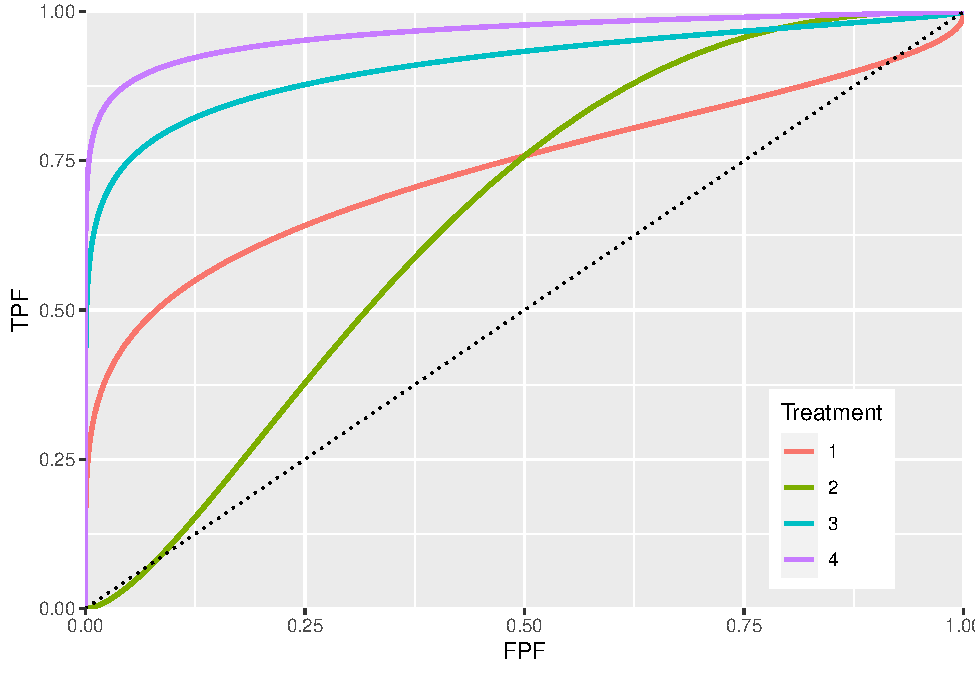
\includegraphics{myReport_files/figure-latex/unnamed-chunk-1-1.pdf}

\begin{Shaded}
\begin{Highlighting}[]
\CommentTok{\# source(here("R/example2.R"))}
\KeywordTok{print}\NormalTok{(}\KeywordTok{head}\NormalTok{(}\KeywordTok{data.frame}\NormalTok{(x,y)))}
\CommentTok{\#\textgreater{}   x         y}
\CommentTok{\#\textgreater{} 1 1 0.9128558}
\CommentTok{\#\textgreater{} 2 2 2.1929531}
\CommentTok{\#\textgreater{} 3 3 4.9616995}
\CommentTok{\#\textgreater{} 4 4 1.9122270}
\CommentTok{\#\textgreater{} 5 5 4.4296145}
\CommentTok{\#\textgreater{} 6 6 6.1725955}
\end{Highlighting}
\end{Shaded}

\hypertarget{DBMHnalysis}{%
\chapter{Dorfman Berbaum Metz Hillis (DBMH) Analysis}\label{DBMHnalysis}}

\hypertarget{introduction}{%
\section{Introduction}\label{introduction}}

In this chapter the term ``treatment'' is used as a generic for ``imaging system'', ``modality'' or ``image processing'' and ``reader'' is used as a generic for ``radiologist'' or algorithmic observer, e.g., a computer aided detection (CAD) algorithm. In the context of illustrating hypothesis-testing methods the previous chapter described analysis of a single ROC dataset and comparing the observed area \(AUC\) under the ROC plot to a specified value. Clinically this is not the most interesting problem; rather, interest is usually in comparing performance of a group of readers interpreting a common set of cases in two or more treatments. Such data is termed multiple reader multiple case (MRMC). {[}An argument could be made in favor of the term ``multiple-treatment multiple-reader'', since ``multiple-case'' is implicit in any ROC analysis that takes into account correct and incorrect decisions on cases. However, the author will stick with existing terminology.{]} The basic idea is that by sampling a sufficiently large number of readers and a sufficiently large number of cases one might be able to draw conclusions that apply broadly to other readers of similar skill levels interpreting other similar case sets in the selected treatments. How one accomplishes this, termed MRMC analysis, is the subject of this chapter.

This chapter describes the first truly successful method of analyzing MRMC ROC data, namely the Dorfman-Berbaum-Metz (DBM) method \citep{RN204}. The other method, due to Obuchowski and Rockette \citep{RN1450}, is the subject of Chapter 10. Both methods have been substantially improved by Hillis \citep{RN1866, RN1865, RN2508}. Hence the title of this chapter: ``Dorfman Berbaum Metz Hillis (DBMH) Analysis''. It is not an overstatement that ROC analysis came of age with the methods described in this chapter. Prior to the techniques described here, one knew of the existence of sources of variability affecting a measured \(AUC\) value, as discussed in (book) Chapter 07, but then-known techniques \citep{RN412} for estimating the corresponding variances and correlations were impractical.

\hypertarget{historical-background}{%
\subsection{Historical background}\label{historical-background}}

The author was thrown (unprepared) into the methodology field ca. 1985 when, as a junior faculty member, he undertook comparing a prototype digital chest-imaging device (Picker International, ca. 1983) vs.~an optimized analog chest-imaging device at the University of Alabama at Birmingham. At the outset a decision was made to use free-response ROC methodology instead of ROC, as the former accounted for lesion localization, and the author and his mentor, Prof.~Gary T. Barnes, were influenced in that decision by a publication \citep{RN2453} to be described in (book) Chapter 12. Therefore, instead of ROC-AUC one had lesion-level sensitivity at a fixed number of location level false positives per case as the figure-of-merit (FOM). Details of the FOM are not relevant at this time. Suffice to state that methods described in this chapter, which had not been developed in 1983, while developed for analyzing reader-averaged inter-treatment ROC-AUC differences, \emph{apply to any scalar FOM}. While the author was successful at calculating confidence intervals (this is the heart of what is loosely termed ``statistical analysis'') and publishing the work \citep{RN621} using techniques described in a book \citep{RN412} titled ``Evaluation of Diagnostic Systems: Methods from Signal Detection Theory'', subsequent attempts at applying these methods in a follow-up paper \citep{RN620} led to negative variance estimates (private communication, Dr.~Loren Niklason, ca. 1985). With the benefit of hindsight, negative variance estimates are not that uncommon and the method to be described in this chapter has to deal with that possibility.

The methods \citep{RN412} described in the cited book involved estimating the different variability components -- case sampling, between-reader and within-reader variability. Between-reader and within-reader variability (the two cannot be separated as discussed in (book) Chapter 07) could be estimated from the variance of the \(AUC\) values corresponding to the readers interpreting the cases within a treatment and then averaging the variances over all treatments. Estimating case-sampling and within-reader variability required splitting the dataset into a few smaller subsets (e.g., a case set with 60 cases might be split into 3 sub-sets of 20 cases each), analyzing each subset to get an \(AUC\) estimate and calculating the variance of the resulting \(AUC\) values \citep{RN412} and scaling the result to the original case size. Because it was based on few values, the estimate was inaccurate, and the already case-starved original dataset made it difficult to estimate AUCs for the subsets; moreover, the division into subsets was at the discretion of the researcher, and therefore unlikely to be reproduced by others. Estimating within-reader variability required re-reading the entire case set, or at least a part of it. ROC studies have earned a deserved reputation for taking much time to complete, and having to re-read a case set was not a viable option. {[}Historical note: the author recalls a barroom conversation with Dr.~Thomas Mertelmeir after the conclusion of an SPIE meeting ca. 2004, where Dr.~Mertelmeir commiserated mightily, over several beers, about the impracticality of some of the ROC studies required of imaging device manufacturers by the FDA.{]}

\hypertarget{the-wagner-analogy}{%
\subsection{The Wagner analogy}\label{the-wagner-analogy}}

An important objective of modality comparison studies is to estimate the variance of the difference in reader-averaged AUCs between the treatments. For two treatments one sums the reader-averaged variance in each treatment and subtracts twice the covariance (a scaled version of the correlation). Therefore, in addition to estimating variances, one needs to estimate correlations. Correlations are present due to the common case set interpreted by the readers in the different treatments. If the correlation is large, i.e., close to unity, then the individual treatment variances tend to cancel, making the constant treatment-induced difference easier to detect. The author recalls a vivid analogy used by the late Dr.~Robert F. Wagner to illustrate this point at an SPIE meeting ca. 2008. To paraphrase him, \emph{consider measuring from shore the heights of the masts on two adjacent boats in a turbulent ocean. Because of the waves, the heights, as measured from shore, are fluctuating wildly, so the variance of the individual height measurements is large. However, the difference between the two heights is likely to be relatively constant, i.e., have small variance. This is because the wave that causes one mast's height to increase also increases the height of the other mast.}

\hypertarget{the-shortage-of-numbers-to-analyze-and-a-pivotal-breakthrough}{%
\subsection{The shortage of numbers to analyze and a pivotal breakthrough}\label{the-shortage-of-numbers-to-analyze-and-a-pivotal-breakthrough}}

\emph{The basic issue was that the calculation of \(AUC\) reduces the relatively large number of ratings of a set of non-diseased and diseased cases to a single number.} For example, after completion of an ROC study with 5 readers and 100 non-diseased and 100 diseased cases interpreted in two treatments, the data is reduced to just 10 numbers, i.e., five readers times two treatments. It is difficult to perform statistics with so few numbers. The author recalls a conversation with Prof.~Kevin Berbaum at a Medical Image Perception Society meeting in Tucson, Arizona, ca. 1997, in which he described the basic idea that forms the subject of this chapter. Namely, using the jackknife pseudovalues, Eqn. (7.6), as individual case-level figures of merit. This, of course, greatly increases the amount of data that one can work with; instead of just 10 numbers one now has 2,000 pseudovalues (2 x 5 x 200). If one assumes the pseudovalues behave essentially as case-level data, then by assumption they are independent and identically distributed , and therefore they satisfy the conditions for application of standard analysis of variance (ANOVA) techniques10. The relevant paper1 had already been published in 1992 but other distractions and lack of formal statistical training kept the author from fully appreciating this work until later.

Although methods are available for more complex study designs including partially paired data \citep{RN2128, RN1880}, I will restrict to fully paired data (i.e., each case is interpreted by all readers in all treatments). There is a long history of how this field has evolved and the author cannot do justice to all methods that are currently available. Some of the methods \citep{RN1441, RN2013, RN1451} have the advantage that they can handle explanatory variables (termed covariates) that could influence performance, e.g., years of experience, types of cases, etc. Other methods are restricted to specific choices of FOM. Specifically, the probabilistic approach \citep{RN2253, RN2254, RN2351, RN2080} is restricted to the empirical \(AUC\) under the ROC curve, and therefore are not applicable to other FOMs, e.g., parametrically fitted ROC AUCs or, more importantly, to location specific paradigm FOMs. Instead, the author will focus on methods for which software is readily available (i.e., freely on websites), which have been widely used (the method that the author is about to describe has been used in several hundred publications) and validated via simulations, and which apply to any scalar figure of merit, and therefore widely applicable, even to location specific paradigms.

\hypertarget{organization-of-the-chapter}{%
\subsection{Organization of the chapter}\label{organization-of-the-chapter}}

The organization of the chapter is as follows. The concepts of reader and case populations, introduced in (book) Chapter 07, are recapitulated. A distinction is made between \emph{fixed} and \emph{random} factors -- statistical terms with which one must become familiar. Described next are three types of analysis that are possible with MRMC data, depending on which factors are regarded as random and which as fixed. The general approach to the analysis is described. Two methods of analysis are possible: the jackknife pseudovalue-based approach detailed in this chapter and an alternative approach is detailed in Chapter 10. The Dorfman-Berbaum-Metz (DBM) model for the jackknife pseudovalues is described that incorporates different sources of variability and correlations possible with MRMC data. Calculation of ANOVA-related quantities, termed mean squares, from the pseudovalues, are described followed by the significance testing procedure for testing the null hypothesis of no treatment effect. A relevant distribution used in the analysis, namely the F-distribution, is illustrated with R examples. The decision rule, i.e., whether to reject the NH, calculation of the ubiquitous p-value, confidence intervals and how to handle multiple treatments is illustrated with two datasets, one an older ROC dataset that has been widely used to demonstrate advances in ROC analysis, and the other a recent dataset involving evaluation of digital chest tomosynthesis vs.~conventional chest imaging. The approach to validation of DBMH analysis is illustrated with an R example. The chapter concludes with a section on the meaning of the pseudovalues. The intent is to explain, at an intuitive level, why the DBM method ``works'', even though use of pseudovalues has been questioned3 at the conceptual level. For organizational reasons and space limitations, details of the software are relegated to Online Appendices, but they are essential reading, preferably in front of a computer running the online software that is part of this book. The author has included material here that may be obvious to statisticians, e.g., an explanation of the Satterthwaite approximation, but are expected to be helpful to others from non-statistical backgrounds.

\hypertarget{random-and-fixed-factors}{%
\section{Random and fixed factors}\label{random-and-fixed-factors}}

\emph{This paragraph introduces some analysis of variance (ANOVA) terminology. Treatment, reader and case are factors with different numbers of levels corresponding to each factor. For an ROC study with two treatments, five readers and 200 cases, there are two levels of the treatment factor, five levels of the reader factor and 200 levels of the case factor. If a factor is regarded as fixed, then the conclusions of the analysis apply only to the specific levels of the factor used in the study. If a factor is regarded as random, the levels of the factor are regarded as random samples from a parent population of the corresponding factor and conclusions regarding specific levels are not allowed; rather, conclusions apply to the distribution from which the levels are, by assumption, sampled.}

ROC MRMC studies require a sample of cases and interpretations by one or more readers in one or more treatments (in this book the term ``multiple'' includes as a special case ``one''). A study is never conducted on a sample of treatments. It would be nonsensical to image patients using a ``sample'' of all possible treatments known to exist. Every variation of an imaging technique (e.g., different kilovoltage or kVp) or display method (e.g., window-level setting) or image processing techniques qualifies as a distinct treatment. The number of possible treatments is very large, and, from a practical point of view, most of them are uninteresting. Rather, interest is in comparing two or more (a few at most) treatments that, based on preliminary studies, are clinically interesting. One treatment may be computed tomography, the other magnetic resonance imaging, or one may be interested in comparing a standard image processing method to a newly proposed one, or one may be interested in comparing CAD to a group of readers.

This brings out an essential difference between how cases, readers and treatments have to be regarded in the variability estimation procedure. Cases and readers are usually regarded as random factors (there has to be at least one random factor -- if not, there are no sources of variability and nothing to apply statistics to!), while treatments are regarded as fixed factors. The random factors contribute stochastic (i.e., random) variability, but the fixed factors do not, rather they contribute constant shifts in performance. The terms fixed and random factors are used in this specific sense, and are derived, in turn, from ANOVA methods in statistics10,25. With two or more treatments, there are shifts in performance of treatments relative to each other, that one seeks to assess the significance of against a background of noise contributed by the random factors. If the shifts are sufficiently large compared to the noise, then one can state, with some certainty, that they are real. Quantifying the last statement uses the methods of hypothesis testing introduced in Chapter \ref{HypothesisTesting} or Chapter {[}Hypothesis Testing{]}.

\hypertarget{reader-and-case-populations-and-data-correlations}{%
\section{Reader and case populations and data correlations}\label{reader-and-case-populations-and-data-correlations}}

As discussed in (book) §7.2, conceptually there is a reader-population, generally modeled as a normal distribution \(\theta_j \sim N\left ( \theta_{\bullet\{1\}}, \sigma_{br+wr}^{2} \right )\), describing the variation of skill-level of readers. The notation closely follows that in the cited section, the only change being that the binormal model estimate \(A_z\) has been replaced by a generic FOM, denoted \(\theta\). Each reader \(j\) is characterized by a different value of \(\theta_j\), \(j=1,2,...J\) and one can conceptually think of a bell-shaped curve with variance \(\sigma_{br+wr}^{2}\) describing between-reader variability of the readers. A large variance implies large spread in reader skill levels.

Likewise, there is a case-population, also modeled as a normal distribution, describing the variations in difficulty levels of the patients. One actually has two unit-variance distributions, one per diseased state, characterized by a separation parameter and conceptually an easy case set has a larger than usual separation parameter while a difficult case set has a smaller than usual separation parameter. The distribution of the separation parameter can be modeled as a bell-shaped curve \(\theta_{\{c\}} \sim N\left ( \theta_{\{\bullet\}}, \sigma_{cs+wr}^{2} \right )\) with variance \(\sigma_{cs+wr}^{2}\) describing the variations in difficulty levels of different case samples. Note the need for the case-set index, introduced in Chapter 07, to specify the separation parameter for a specific case-set (in principle a \(j\)-index is also needed as one cannot have an interpretation without a reader; for now it is suppressed; one can think of the stated equation as applying to the average reader). A small variance \(\sigma_{cs}^{2}\) implies the different case sets have similar difficulty levels while a larger variance would imply a larger spread in difficulty levels.

\emph{Anytime one has a common random component to two measurements, the measurements are correlated.} In the Wagner analogy, the common component is the random height, as a function of time, of a wave, which contributes the same amount to both height measurements (since the boats are adjacent). Since the readers interpret a common case set in all treatments one needs to account for various types of correlations that are potentially present. These occur due to the various types of pairings that can occur with MRMC data, where each pairing implies the presence of a common component to the measurements: (a) the same reader interpreting the same cases in different treatments, (b) different readers interpreting the same cases in the same treatment and (c) different readers interpreting the same cases in different treatments. These pairings are more clearly elucidated in (book) Chapter 10. The current chapter uses jackknife pseudovalue based analysis to model the variances and the correlations. Hillis has shown that the two approaches are essentially equivalent \citep{RN1866}.

\hypertarget{three-types-of-analyses}{%
\section{Three types of analyses}\label{three-types-of-analyses}}

\emph{MRMC analysis attempts to draw conclusions regarding the significances of inter-treatment shifts in performance. Ideally a conclusion (i.e., a difference is significant: yes/no; the ``yes'' applies if the p-value is less than alpha) should generalize to the respective populations from which the random samples were obtained. In other words, the idea is to generalize from the observed samples to the underlying populations. Three types of analyses are possible depending on which factor(s) one regards as random and which as fixed: random-reader random-case (RRRC), fixed-reader random-case (FRRC) and random-reader fixed-case (RRFC). If a factor is regarded as random, then the conclusion of the study applies to the population from which the levels of the factor were sampled. If a factor is regarded as fixed, then the conclusion applies only to the specific levels of the sampled factor. For example, if reader is regarded as a random factor, the conclusion generalizes to the reader population from which the readers used in the study were obtained. If reader is regarded as a fixed factor, then the conclusion applies to the specific readers that participated in the study. Regarding a factor as fixed effectively ``freezes out'' the sampling variability of the population and interest then centers only on the specific levels of the factor used in the study. For fixed reader analysis, conclusions about the significances of differences between pairs of readers are allowed; these are not allowed if reader is treated as a random factor. Likewise, treating case as a fixed factor means the conclusion of the study is specific to the case-set used in the study.}

\hypertarget{general-approach}{%
\section{General approach}\label{general-approach}}

This section provides an overview of the steps involved in analysis of MRMC data. Two approaches are described in parallel: a figure of merit (FOM) derived jackknife pseudovalue based approach, detailed in this chapter and an FOM based approach, detailed in the next chapter. The analysis proceeds as follows:

\begin{enumerate}
\def\labelenumi{\arabic{enumi}.}
\tightlist
\item
  A FOM is selected: \emph{the selection of FOM is the single-most critical aspect of analyzing an observer performance study}. The selected FOM is denoted \(\theta\). To keep the notation reasonably compact the usual circumflex ``hat'' symbol used previously to denote an estimate is suppressed. The FOM has to be an objective scalar measure of performance with larger values characterizing better performance. {[}The qualifier ``larger'' is trivially satisfied; if the figure of merit has the opposite characteristic, a sign change is all that is needed to bring it back to compliance with this requirement.{]} Examples are empirical \(AUC\), the binormal model-based estimate \(A_z\) , other advance method based estimates of \(AUC\), sensitivity at a predefined value of specificity, etc. An example of a FOM requiring a sign-change is \(FPF\) at a specified \(TPF\), where smaller values signify better performance.
\item
  For each treatment \(i\) and reader \(j\) the figure of merit \(\theta_{ij}\) is estimated from the ratings data. Repeating this over all treatments and readers yields a matrix of observed values \(\theta_{ij}\). This is averaged over all readers in each treatment yielding \(\theta_{i\bullet}\). The observed effect-size \(ES_{obs}\) is defined as the difference between the reader-averaged FOMs in the two treatments, i.e., \(ES_{obs}\) = \(\theta_{2\bullet}\) - \(\theta_{1\bullet}\). While extensible to more than two treatments, the explanation is more transparent by restricting to two modalities.
\item
  If the magnitude of \(ES_{obs}\) is ``large'' one has reason to suspect that there might indeed be a significant difference in AUCs between the two treatments, where significant is used in the sense of (book) Chapter 08. Quantification of this statement, specifically how large is ``large'', requires the conceptually more complex steps described next.
\end{enumerate}

\begin{itemize}
\tightlist
\item
  In the DBMH approach, the subject of this chapter, jackknife pseudovalues are calculated as described in Chapter 08. A standard ANOVA model with uncorrelated errors is used to model the pseudovalues.
\item
  In the ORH approach, the subject of the next chapter, the FOM is modeled directly using a custom ANOVA model with correlated errors.
\end{itemize}

\begin{enumerate}
\def\labelenumi{\arabic{enumi}.}
\tightlist
\item
  Depending on the selected method of modeling the data (pseudovalue vs.~FOM) a statistical model is used which includes parameters modeling the true values in each treatment, and expected variations due to different variability components in the model, e.g., between-reader variability, case-sampling variability, interactions (e.g., modeling the possibility that the random effect of a given reader could be treatment dependent) and the presence of correlations (between pseudovalues or FOMs) because of the pairings inherent in the interpretations.
\item
  In RRRC analysis one accounts for randomness in readers and cases. In FRRC analysis one regards reader as a fixed factor. In RRFC analysis one regards case as a fixed factor. The statistical model depends on the type of analysis.
\item
  The parameters of the statistical model are estimated from the observed data.
\item
  The estimates are used to infer the statistical distribution of the observed effect size, \(ES_{obs}\), regarded as a realization of a random variable, under the null hypothesis (NH) that the true effect size is zero.
\item
  Based on this statistical distribution, and assuming a two-sided test, the probability (this is the oft-quoted p-value) of obtaining an effect size at least as extreme as that actually observed, is calculated, as in Chapter 08.
\item
  If the p-value is smaller than a preselected value, denoted \(\alpha\), one declares the treatments different at the \(\alpha\) - significance level. The quantity \(\alpha\) is the control (or cap) on the probability of making a Type I error, defined as rejecting the NH when it is true. It is common to set \(\alpha\) = 0.05 but depending on the severity of the consequences of a Type I error, as discussed in (book) Chapter 08, one might consider choosing a different value. Notice that \(\alpha\) is a pre-selected number while the p-value is a realization of a random variable.
\item
  For a valid statistical analysis, the empirical probability \(\alpha_{emp}\) over many (typically 2000) independent NH datasets, that the p-value is smaller than \(\alpha\), should equal \(\alpha\) to within statistical uncertainty.
\end{enumerate}

\hypertarget{the-dorfman-berbaum-metz-dbm-method}{%
\section{The Dorfman-Berbaum-Metz (DBM) method}\label{the-dorfman-berbaum-metz-dbm-method}}

The figure-of-merit has three indices:\\
1. A treatment index \(i\), where \(i\) runs from 1 to \(I\), where \(I\) is the total number of treatments.
1. A reader index \(j\), where \(j\) runs from 1 to \(J\), where \(J\) is the total number of readers.
1. The often-suppressed case-sample index \(\{c\}\), where \(\{1\}\) i.e., \(c\) = 1, denotes a set of cases, \(K_1\) non-diseased and \(K_2\) diseased, interpreted by all readers in all treatments, and other integer values of \(c\) correspond to other independent sets of cases that, although not in fact interpreted by the readers, could potentially be ``interpreted'' using resampling methods such as the bootstrap or the jackknife.

The approach \citep{RN204} taken by Dorfman-Berbaum-Metz (DBM) was to use the jackknife resampling method described in (book) Chapter 7 to calculate FOM pseudovalues \({Y'}_{ijk}\) defined by (the reason for the prime will become clear shortly):

\begin{equation*}
Y'_{ijk}=K\theta_{ij}-(K-1)\theta_{ij\{k\}}
\end{equation*}

Here \(\theta_{ij}\) is the estimate of the figure-of-merit for reader \(j\) interpreting all cases in treatment \(i\) and \(\theta_{ij\{k\}}\) is the corresponding figure of merit with case \(k\) \emph{deleted} from the analysis. To adhere to convention and to keep the notation simple the \(\{1\}\) index on every figure of merit symbol is suppressed (unless it is absolutely necessary for clarity).

Recall from book Chapter 07 that the jackknife is a way of teasing out the case-dependence: the left hand side of Eqn. (9.1) literally has a case index \(k\), with \(k\) running from 1 to \(K\), where \(K\) is the total number of cases: \(K=K_1+K_2\).

Hillis has proposed a centering transformation on the pseudovalues (Hillis calls them ``normalized'' pseudovalues but to the author ``centering'' is a more accurate and descriptive term - \emph{Normalize: (In mathematics) multiply (a series, function, or item of data) by a factor that makes the norm or some associated quantity such as an integral equal to a desired value (usually 1). New Oxford American Dictionary, 2016}):

\begin{equation*}
Y_{ijk}=Y'_{ijk}+\left (\theta_{ij} - Y'_{ij\bullet}  \right )
\end{equation*}

\textbf{Note: the bullet symbol denotes an average over the corresponding index.}

The effect of this transformation is that the average of the centered pseudovalues over the case index is identical to the corresponding estimate of the figure of merit:

\begin{equation*}
Y_{ij\bullet}=Y'_{ij\bullet}+\left (\theta_{ij} - Y'_{ij\bullet}  \right )=\theta_{ij}
\end{equation*}

This has the advantage that all confidence intervals are correctly centered. The transformation is unnecessary if one uses the Wilcoxon as the figure-of-merit, as the pseudovalues calculated using the Wilcoxon as the figure of merit are automatically centered. It is left as an exercise for the reader to show that this statement is true.

\emph{It is understood that, unless explicitly stated otherwise, all calculations from now on will use centered pseudovalues.}

Consider \(N\) replications of a MRMC study, where a replication means repetition of the study with the same treatments, readers and case-set \(\{1\}\). For \(N\) replications per treatment-reader-case combination, the DBM model for the pseudovalues is (\(n\) is the replication index, usually \(n\) = 1, but kept here for now):

\begin{equation*}
Y_{n(ijk)}  = \mu + \tau_i+ R_j + C_k + (\tau R)_{ij}+ (\tau C)_{ik}+ (R C)_{jk} + (\tau RC)_{ijk}+ \epsilon_{n(ijk)} 
\end{equation*}

The term \(\mu\) is a constant. By definition, the treatment effect \(\tau_i\) is subject to the constraint:

\begin{equation*}
\sum_{i=1}^{I}\tau_i=0\Rightarrow \tau_\bullet=0
\end{equation*}

It is shown below, Eqn. (9.9), that this constraint ensures that \(\mu\) has the interpretation as the average of the pseudovalues over treatments, readers, cases and replications, if any.

The notation for the replication index, i.e., \(n(ijk)\), implies \(n\) observations for treatment-reader-case combination \(ijk\). With no replications (\(N\) = 1) it is convenient to omit the n-symbol. As an example, the parameter \(\tau_i\) is readily estimated as follows:

\begin{equation}
\theta_{ij\{c\}}=\mu+\tau_i+R_j+(\tau R)_{ij}+\epsilon_{ij\{c\}}
\end{equation}

\[
Y_{ijk}\equiv Y_{1(ijk)}\\
\tau_i = Y_{i \bullet \bullet} -Y_{\bullet \bullet \bullet} 
\]

\emph{The basic assumption of the DBM model, Eqn. (9.4), is that the pseudovalues can be regarded as independent and identically distributed observations. That being the case, the pseudovalues can be analyzed by standard ANOVA techniques.}

\hypertarget{explanation-of-terms-in-the-model}{%
\subsection{Explanation of terms in the model}\label{explanation-of-terms-in-the-model}}

The right hand side of Eqn. (9.4) consists of one fixed and 7 random effects. The current analysis assumes readers and cases as random factors (RRRC), so by definition \(R_j\) and \(C_k\) are random effects, and moreover, any term that includes a random factor is a random effect; for example, \((\tau R)_{ij}\) is a random effect because it includes the \(R\) factor. Here is a list of the random terms:

\[
R_j, C_k, (\tau R)_{ij}, (\tau C)_{ik}, (RC)_{jk},  (\tau RC)_{ijk},  \epsilon_{ijk}
\]

\textbf{Assumption:} Each of the random effects is modeled as a random sample from mutually independent zero-mean normal distributions with variances as specified below:

\[
R_j  \sim N\left ( 0,\sigma_{R}^{2} \right ) \\
C_k \sim N\left ( 0,\sigma_{C}^{2} \right ) \\
(\tau R)_{ij} \sim N\left ( 0,\sigma_{\tau R}^{2} \right ) \\
(\tau C)_{ik} \sim N\left ( 0,\sigma_{\tau C}^{2} \right ) \\
(RC)_{jk} \sim N\left ( 0,\sigma_{RC}^{2} \right ) \\
(\tau RC)_{ijk} \sim N\left ( 0,\sigma_{\tau RC}^{2} \right ) \\
\epsilon_{ijk} \sim N\left ( 0,\sigma_{\epsilon}^{2} \right )
\]

One could have placed a \(Y\) subscript (or superscript) on each of the variances, as they describe fluctuations of the pseudovalues, not FOM values -- the latter are the subject of the next chapter. However, this tends to make the notation cumbersome. So here is the convention:

\emph{Unless explicitly stated otherwise, all variance symbols in this chapter refer to pseudovalues. }

Another convention: \((\tau R)_{ij}\) is \emph{not} the product of the treatment and reader factors, rather it is a single factor, namely the treatment-reader factor with \(IJ\) levels, subscripted by the index \(ij\) and similarly for the other product-like terms in Eqn. (9.7).

\hypertarget{meanings-of-variance-components-in-the-dbm-model-tba-this-section-can-be-improved}{%
\subsection{Meanings of variance components in the DBM model (TBA this section can be improved)}\label{meanings-of-variance-components-in-the-dbm-model-tba-this-section-can-be-improved}}

The variances defined in Eqn. (9.7) are collectively termed variance components. Specifically, they are jackknife pseudovalue variance components, to be distinguished from figure of merit (FOM) variance components to be introduced in Chapter 10. They are in order: \(\sigma_{R}^{2} ,\sigma_{C}^{2} \sigma_{\tau R}^{2},\sigma_{\tau C}^{2},\sigma_{RC}^{2}, \sigma_{\tau RC}^{2},\sigma_{\epsilon}^{2}\). They have the following meanings (all references to ``variance'' mean ``variance of pseudovalues'').

\begin{itemize}
\tightlist
\item
  The term \(\sigma_{R}^{2}\) is the variance of readers that is independent of treatment or case, which are modeled separately. It is not to be confused with the terms \(\sigma_{br+wr}^{2}\) and \(\sigma_{cs+wr}^{2}\) used in §9.3, which describe the variability of \(\theta\) measured under specified conditions. {[}A jackknife pseudovalue is a weighted difference of FOM like quantities, Eqn. (9.1). Its meaning will be explored later. For now, \emph{a pseudovalue variance is distinct from a FOM variance}.{]}
\item
  The term \(\sigma_{C}^{2}\) is the variance of cases that is independent of treatment or reader.
\item
  The term \(\sigma_{\tau R}^{2}\) is the treatment-dependent variance of readers that was excluded in the definition of \(\sigma_{R}^{2}\). If one were to sample readers and treatments for the same case-set, the net variance would be \(\sigma_{R}^{2}+\sigma_{\tau R}^{2}+\sigma_{\epsilon}^{2}\).
\item
  The term \(\sigma_{\tau C}^{2}\) is the treatment-dependent variance of cases that was excluded in the definition of \(\sigma_{C}^{2}\). So, if one were to sample cases and treatments for the same readers, the net variance would be \(\sigma_{C}^{2}+\sigma_{\tau C}^{2}+\sigma_{\epsilon}^{2}\).
\item
  The term \(\sigma_{RC}^{2}\) is the treatment-independent variance of readers and cases that were excluded in the definitions of \(\sigma_{R}^{2}\) and \(\sigma_{C}^{2}\). So, if one were to sample readers and cases for the same treatment, the net variance would be \(\sigma_{R}^{2}+\sigma_{C}^{2}+\sigma_{RC}^{2}+\sigma_{\epsilon}^{2}\).
\item
  The term \(\sigma_{\tau RC}^{2}\) is the variance of treatments, readers and cases that were excluded in the definitions of all the preceding terms in Eqn. (9.7). So, if one were to sample treatments, readers and cases the net variance would be \(\sigma_{R}^{2}+\sigma_{C}^{2}+\sigma_{\tau C}^{2}+\sigma_{RC}^{2}+\sigma_{\tau RC}^{2}+\sigma_{\epsilon}^{2}\).
\item
  The last term, \(\sigma_{\epsilon}^{2}\) describes the variance arising from different replications of the study using the same treatments, readers and cases. Measuring this variance requires repeating the study several (\(N\)) times with the same treatments, readers and cases, and computing the variance of \(Y_{n(ijk)}\) , where the additional \(n\)-index refers to true replications, \(n\) = 1, 2, \ldots, \(N\).
\end{itemize}

\[
\sigma_{\epsilon}^{2}=\frac{1}{IJK}\sum_{i=1}^{I}\sum_{j=1}^{J}\sum_{k=1}^{k}\frac{1}{N-1}\sum_{n=1}^{N}\left ( Y_{n(ijk)} - Y_{\bullet (ijk)} \right )^2
\]

The right hand side of Eqn. (9.8) is the variance of \(Y_{n(ijk)}\), for specific \(ijk\), with respect to the replication index \(n\), averaged over all \(ijk\). In practice \(N\) = 1 (i.e., there are no replications) and this variance cannot be estimated (it would imply dividing by zero). It has the meaning of \emph{reader inconsistency}, usually termed \emph{within-reader} variability. As will be shown later, the presence of this inestimable term does not limit ones ability to perform significance testing on the treatment effect without having to replicate the whole study, as implied in earlier work \citep{RN1450}.

An equation like Eqn. (9.7) is termed a \emph{linear model} with the left hand side, the pseudovalue ``observations'', modeled by a sum of fixed and random terms. Specifically it is a \emph{mixed model}, because the right hand side has both fixed and random effects. Statistical methods have been developed for analysis of such linear models. One estimates the terms on the right hand side of Eqn. (9.7), it being understood that for the random effects, one estimates the variances of the zero-mean normal distributions, Eqn. (9.7), from which the samples are obtained (by assumption).

Estimating the fixed effects is trivial. The term \(\mu\) is estimated by averaging the left hand side of Eqn. (9.4) over all three indices (since \(N\) = 1): \(\mu=Y_{\bullet \bullet \bullet}\)

Because of the way the treatment effect is defined, Eqn. (9.5), averaging, which involves summing, over the treatment-index \(i\), yields zero, and all of the remaining random terms yield zero upon averaging, because they are individually sampled from zero-mean normal distributions. To estimate the treatment effect one takes the difference \(\tau_i=Y_{\bullet \bullet \bullet}-\mu\).

It can be easily seen that the reader and case averaged difference between two different treatments \(i\) and \(i'\) is estimated by \(\tau_i-\tau_{i'} = Y_{i \bullet \bullet} - Y_{i' \bullet \bullet}\).

Estimating the strengths of the random terms is a little more complicated. It involves methods adapted from least squares, or maximum likelihood, and more esoteric ways. I do not feel comfortable going into these methods. Instead, results are presented and arguments are made to make them plausible. The starting point is definitions of quantities called \textbf{mean squares} and their expected values.

\hypertarget{definitions-of-mean-squares}{%
\subsection{Definitions of mean-squares}\label{definitions-of-mean-squares}}

Again, to be clear, one should put a \(Y\) subscript (or superscript) on each of the following definitions, but that would make the notation unnecessarily cumbersome.

\emph{In this chapter, all mean-square quantities are calculated using pseudovalues, not figure-of-merit values. The presence of three subscripts on Y should make this clear. Also the replication index and the nesting notation are suppressed. The notation is abbreviated so MST is the mean square corresponding to the treatment effect, etc.}

The definitions of the mean-squares below match those (when provided) in \citep[page 1261]{RN1476}; the definition of \(MS(R)\) in \citep[top of page 339]{RN2508} is incorrect.

\begin{equation*}
\text{MS(T)}=\frac{JK\sum_{i=1}^{I}\left ( Y_{i \bullet \bullet} - Y_{ \bullet \bullet \bullet} \right )^2}{I-1} \\
\text{MS(R)}=\frac{IK\sum_{j=1}^{J}\left ( Y_{\bullet j \bullet} - Y_{ \bullet \bullet \bullet} \right )^2}{J-1} \\
\text{MS(C)}=\frac{IJ\sum_{k=1}^{K}\left ( Y_{\bullet \bullet k} - Y_{ \bullet \bullet \bullet} \right )^2}{K-1} \\
\text{MS(TR)}=\frac{K\sum_{i=1}^{I}\sum_{j=1}^{J}\left ( Y_{i j \bullet} - Y_{i \bullet \bullet} - Y_{\bullet j \bullet} + Y_{ \bullet \bullet \bullet} \right )^2}{(I-1)(J-1)} \\
\text{MS(TC)}=\frac{J\sum_{i=1}^{I}\sum_{k=1}^{K}\left ( Y_{i \bullet k} - Y_{i \bullet \bullet} - Y_{\bullet \bullet k} + Y_{ \bullet \bullet \bullet} \right )^2}{(I-1)(K-1)} \\
\text{MS(RC)}=\frac{I\sum_{j=1}^{J}\sum_{k=1}^{K}\left ( Y_{\bullet j k} - Y_{\bullet j \bullet} - Y_{\bullet \bullet k} + Y_{ \bullet \bullet \bullet} \right )^2}{(J-1)(K-1)}\\
\text{MS(TRC)}=\frac{\sum_{i=1}^{I}\sum_{j=1}^{J}\sum_{k=1}^{K}\left ( Y_{i j k} - Y_{i j \bullet} - Y_{i \bullet k} - Y_{\bullet j k} + Y_{i \bullet \bullet} + Y_{\bullet j \bullet} + Y_{\bullet \bullet k} - Y_{ \bullet \bullet \bullet} \right )^2}{(I-1)(J-1)K-1)}
\end{equation*}

Note the absence of \(MSE\), corresponding to the \(\epsilon\) term on the right hand side of Eqn. (9.4). With only one observation per treatment-reader-case combination, MSE cannot be estimated; it effectively gets folded into the \(MS(TRC)\) term.

\hypertarget{expected-values-of-mean-squares}{%
\section{Expected values of mean squares}\label{expected-values-of-mean-squares}}

\begin{quote}
``In our original formulation {[}2{]}, expected mean squares for the ANOVA were derived from a restricted parameterization in which mixed-factor interactions sum to zero over indexes of fixed effects. In the restricted parameterization, the mixed effects are correlated, parameters are sometimes awkward to define {[}17{]}, and extension to unbalanced designs is dubious {[}17, 18{]}. In this article, we recommend the unrestricted parameterization. The restricted and unrestricted parameterizations are special cases of a general model by Scheffe {[}19{]} that allows an arbitrary covariance structure among experimental units within a level of a random factor. Tables 1 and 2 show the ANOVA tables with expected mean squares for the unrestricted formulation.''

--- \citep{RN2079}
\end{quote}

The mean squares on the left hand side of Eqn. (9.12) can be calculated directly from the pseudovalues. The next step in the analysis is to obtain expressions for their expected values in terms of the variances defined in Eqn. (9.7). Assuming no replications, i.e., \(N\) = 1, the expected mean squares are as follows, Table 9.1; understanding how this table is derived, would lead the author well outside his expertise and the scope of this book; suffice to say that these are \emph{unconstrained} estimates (as summarized in the quotation above) which are different from the \emph{constrained} estimates appearing in the original DBM publication \citep{RN204}.

\begin{longtable}[]{@{}lll@{}}
\caption{Table 9.1 Unconstrained expected values of mean-squares, as in \citep{RN2079}}\tabularnewline
\toprule
Source & df & E(MS)\tabularnewline
\midrule
\endfirsthead
\toprule
Source & df & E(MS)\tabularnewline
\midrule
\endhead
T & (I-1) & \(\sigma_{\epsilon}^{2}\) + \(\sigma_{\tau RC}^{2}\) + \(K\sigma_{\tau R}^{2}\) + \(J\sigma_{\tau C}^{2}\) + \(JK\sigma_{\tau}^{2}\)\tabularnewline
R & (J-1) & \(\sigma_{\epsilon}^{2}\) + \(I\sigma_{RC}^{2}\) + \(IK\sigma_{R}^{2}\) + \(K\sigma_{\tau R}^{2}\)\tabularnewline
C & (K-1) & \(\sigma_{\epsilon}^{2}\) + \(I\sigma_{RC}^{2}\) + \(IJ\sigma_{C}^{2}\) + \(J\sigma_{\tau C}^{2}\)\tabularnewline
TR & (I-1)(J-1) & \(\sigma_{\epsilon}^{2}\) + \(\sigma_{\tau RC}^{2}\) + \(K\sigma_{\tau R}^{2}\)\tabularnewline
TC & (I-1)(K-1) & \(\sigma_{\epsilon}^{2}\) + \(\sigma_{\tau RC}^{2}\) + \(J\sigma_{\tau C}^{2}\)\tabularnewline
RC & (J-1)(K-1) & \(\sigma_{\epsilon}^{2}\) + \(I\sigma_{RC}^{2}\)\tabularnewline
TRC & (I-1)(J-1)(K-1) & \(\sigma_{\epsilon}^{2}\) + \(\sigma_{\tau RC}^{2}\)\tabularnewline
\(\epsilon\) & \(N-1=0\) & \(\sigma_{\epsilon}^{2}\)\tabularnewline
\bottomrule
\end{longtable}

\begin{itemize}
\tightlist
\item
  In Tables 9.1 the following notation is used as a shorthand:
\end{itemize}

\begin{equation*}
\sigma_{\tau}^{2}=\frac{1}{I-1}\sum_{i=1}^{I}\left ( Y_{i \bullet \bullet} - Y_{\bullet \bullet \bullet} \right )^2
\end{equation*}

\begin{itemize}
\item
  Since treatment is a fixed effect, the variance symbol \(\sigma_{\tau}^{2}\), which is used for notational consistency in Tables 9.1 - 9.3, could cause confusion.
\item
  The right hand side ``looks like'' a variance, indeed one that could be calculated for just two treatments but, of course, random sampling from a \emph{distribution of treatments} is not the intent of the notation. With this explanation, I trust the reader will not be confused.
\end{itemize}

\hypertarget{random-reader-random-case-rrrc-analysis}{%
\section{Random-reader random-case (RRRC) analysis}\label{random-reader-random-case-rrrc-analysis}}

Both readers and cases are regarded as random factors. The expected mean squares in Table 9.1 are variance-like quantities; specifically, they are weighted linear combinations of the variances appearing in Eqn. (9.7). For single factors the column headed ``degrees of freedom'' (\(df\)) is one less than the number of levels of the corresponding factor; estimating a variance requires first estimating the mean, which imposes a constraint, thereby decreasing \(df\) by one. For interaction terms, \(df\) is the product of the degrees of freedom for the individual factors. As an example, the term \((\tau RC)_{ijk}\) contains three individual factors, and therefore \(df = (I-1)(J-1)(K-1)\). The number of degrees of freedom can be thought of as the amount of information available in estimating a mean square. As a special case, with no replications, the \(\epsilon\) term has zero \(df\) as \(N-1 = 0\). With only one observation \(Y_{1(ijk)}\) there is no information to estimate the variance corresponding to the \(\epsilon\) term. To estimate this term one needs to replicate the study several times -- each time the same readers interpret the same cases in all treatments -- a very boring task for the reader and totally unnecessary from the researcher's point of view.

\hypertarget{example-1-calculation-of-mean-squares}{%
\subsection{Example 1: Calculation of mean squares}\label{example-1-calculation-of-mean-squares}}

We choose \texttt{dataset02} to illustrate calculation of mean squares for pseudovalues. This is referred to in the book as the ``VD'' dataset \citep{RN1993}. It consists of 114 cases, 45 of which are diseased, interpreted in two treatments (``0'' = single spin echo MRI, ``1'' = cine-MRI) by five radiologists using the ROC paradigm. The first line below computes the pseudovalues and extracts the numbers of treatmenets, readers and cases, used in the subsequent calculations of mean squares.

\begin{Shaded}
\begin{Highlighting}[]
\NormalTok{Y \textless{}{-}}\StringTok{ }\KeywordTok{UtilPseudoValues}\NormalTok{(dataset02, }\DataTypeTok{FOM =} \StringTok{"Wilcoxon"}\NormalTok{)}\OperatorTok{$}\NormalTok{jkPseudoValues}
\NormalTok{I \textless{}{-}}\StringTok{ }\KeywordTok{dim}\NormalTok{(Y)[}\DecValTok{1}\NormalTok{];J \textless{}{-}}\StringTok{ }\KeywordTok{dim}\NormalTok{(Y)[}\DecValTok{2}\NormalTok{];K \textless{}{-}}\StringTok{ }\KeywordTok{dim}\NormalTok{(Y)[}\DecValTok{3}\NormalTok{]}
\NormalTok{msT \textless{}{-}}\StringTok{ }\DecValTok{0}
\ControlFlowTok{for}\NormalTok{ (i }\ControlFlowTok{in} \DecValTok{1}\OperatorTok{:}\NormalTok{I) \{ }\CommentTok{\# OK}
\NormalTok{  msT \textless{}{-}}\StringTok{ }\NormalTok{msT }\OperatorTok{+}\StringTok{ }\NormalTok{(}\KeywordTok{mean}\NormalTok{(Y[i, , ]) }\OperatorTok{{-}}\StringTok{ }\KeywordTok{mean}\NormalTok{(Y))}\OperatorTok{\^{}}\DecValTok{2}
\NormalTok{\}}
\NormalTok{msT \textless{}{-}}\StringTok{ }\NormalTok{msT }\OperatorTok{*}\StringTok{ }\NormalTok{K }\OperatorTok{*}\StringTok{ }\NormalTok{J}\OperatorTok{/}\NormalTok{(I }\OperatorTok{{-}}\StringTok{ }\DecValTok{1}\NormalTok{)}

\NormalTok{msTC \textless{}{-}}\StringTok{ }\DecValTok{0}
\ControlFlowTok{for}\NormalTok{ (i }\ControlFlowTok{in} \DecValTok{1}\OperatorTok{:}\NormalTok{I) \{}
  \ControlFlowTok{for}\NormalTok{ (k }\ControlFlowTok{in} \DecValTok{1}\OperatorTok{:}\NormalTok{K) \{ }\CommentTok{\# OK}
\NormalTok{    msTC \textless{}{-}}\StringTok{ }\NormalTok{msTC }\OperatorTok{+}\StringTok{ }\NormalTok{(}\KeywordTok{mean}\NormalTok{(Y[i, , k]) }\OperatorTok{{-}}\StringTok{ }\KeywordTok{mean}\NormalTok{(Y[i, , ]) }\OperatorTok{{-}}\StringTok{ }\KeywordTok{mean}\NormalTok{(Y[, , k]) }\OperatorTok{+}\StringTok{ }\KeywordTok{mean}\NormalTok{(Y))}\OperatorTok{\^{}}\DecValTok{2}
\NormalTok{  \}}
\NormalTok{  msTC \textless{}{-}}\StringTok{ }\NormalTok{msTC }\OperatorTok{*}\StringTok{ }\NormalTok{J}\OperatorTok{/}\NormalTok{((I }\OperatorTok{{-}}\StringTok{ }\DecValTok{1}\NormalTok{) }\OperatorTok{*}\StringTok{ }\NormalTok{(K }\OperatorTok{{-}}\StringTok{ }\DecValTok{1}\NormalTok{))}
\NormalTok{\} }

\NormalTok{msR \textless{}{-}}\StringTok{ }\DecValTok{0}
\ControlFlowTok{for}\NormalTok{ (j }\ControlFlowTok{in} \DecValTok{1}\OperatorTok{:}\NormalTok{J) \{ }\CommentTok{\# OK}
\NormalTok{  msR \textless{}{-}}\StringTok{ }\NormalTok{msR }\OperatorTok{+}\StringTok{ }\NormalTok{(}\KeywordTok{mean}\NormalTok{(Y[, j, ]) }\OperatorTok{{-}}\StringTok{ }\KeywordTok{mean}\NormalTok{(Y))}\OperatorTok{\^{}}\DecValTok{2}
\NormalTok{\}}
\NormalTok{msR \textless{}{-}}\StringTok{ }\NormalTok{msR }\OperatorTok{*}\StringTok{ }\NormalTok{K }\OperatorTok{*}\StringTok{ }\NormalTok{I}\OperatorTok{/}\NormalTok{(J }\OperatorTok{{-}}\StringTok{ }\DecValTok{1}\NormalTok{)}

\NormalTok{msC \textless{}{-}}\StringTok{ }\DecValTok{0}
\ControlFlowTok{for}\NormalTok{ (k }\ControlFlowTok{in} \DecValTok{1}\OperatorTok{:}\NormalTok{K) \{ }\CommentTok{\# Not used subsequently}
\NormalTok{  msC \textless{}{-}}\StringTok{ }\NormalTok{msC }\OperatorTok{+}\StringTok{ }\NormalTok{(}\KeywordTok{mean}\NormalTok{(Y[, , k]) }\OperatorTok{{-}}\StringTok{ }\KeywordTok{mean}\NormalTok{(Y))}\OperatorTok{\^{}}\DecValTok{2}
\NormalTok{\}}
\NormalTok{msC \textless{}{-}}\StringTok{ }\NormalTok{msC }\OperatorTok{*}\StringTok{ }\NormalTok{I }\OperatorTok{*}\StringTok{ }\NormalTok{J}\OperatorTok{/}\NormalTok{(K }\OperatorTok{{-}}\StringTok{ }\DecValTok{1}\NormalTok{)}

\NormalTok{msTR \textless{}{-}}\StringTok{ }\DecValTok{0}
\ControlFlowTok{for}\NormalTok{ (i }\ControlFlowTok{in} \DecValTok{1}\OperatorTok{:}\NormalTok{I) \{}
  \ControlFlowTok{for}\NormalTok{ (j }\ControlFlowTok{in} \DecValTok{1}\OperatorTok{:}\NormalTok{J) \{ }\CommentTok{\# OK}
\NormalTok{    msTR \textless{}{-}}\StringTok{ }\NormalTok{msTR }\OperatorTok{+}\StringTok{ }\NormalTok{(}\KeywordTok{mean}\NormalTok{(Y[i, j, ]) }\OperatorTok{{-}}\StringTok{ }\KeywordTok{mean}\NormalTok{(Y[i, , ]) }\OperatorTok{{-}}\StringTok{ }\KeywordTok{mean}\NormalTok{(Y[, j, ]) }\OperatorTok{+}\StringTok{ }\KeywordTok{mean}\NormalTok{(Y))}\OperatorTok{\^{}}\DecValTok{2}
\NormalTok{  \}}
\NormalTok{\}}
\NormalTok{msTR \textless{}{-}}\StringTok{ }\NormalTok{msTR }\OperatorTok{*}\StringTok{ }\NormalTok{K}\OperatorTok{/}\NormalTok{((I }\OperatorTok{{-}}\StringTok{ }\DecValTok{1}\NormalTok{) }\OperatorTok{*}\StringTok{ }\NormalTok{(J }\OperatorTok{{-}}\StringTok{ }\DecValTok{1}\NormalTok{))}

\NormalTok{msTC \textless{}{-}}\StringTok{ }\DecValTok{0}
\ControlFlowTok{for}\NormalTok{ (i }\ControlFlowTok{in} \DecValTok{1}\OperatorTok{:}\NormalTok{I) \{}
  \ControlFlowTok{for}\NormalTok{ (k }\ControlFlowTok{in} \DecValTok{1}\OperatorTok{:}\NormalTok{K) \{ }\CommentTok{\# OK}
\NormalTok{    msTC \textless{}{-}}\StringTok{ }\NormalTok{msTC }\OperatorTok{+}\StringTok{ }\NormalTok{(}\KeywordTok{mean}\NormalTok{(Y[i, , k]) }\OperatorTok{{-}}\StringTok{ }\KeywordTok{mean}\NormalTok{(Y[i, , ]) }\OperatorTok{{-}}\StringTok{ }\KeywordTok{mean}\NormalTok{(Y[, , k]) }\OperatorTok{+}\StringTok{ }\KeywordTok{mean}\NormalTok{(Y))}\OperatorTok{\^{}}\DecValTok{2}
\NormalTok{  \}}
\NormalTok{\}}
\NormalTok{msTC \textless{}{-}}\StringTok{ }\NormalTok{msTC }\OperatorTok{*}\StringTok{ }\NormalTok{J}\OperatorTok{/}\NormalTok{((I }\OperatorTok{{-}}\StringTok{ }\DecValTok{1}\NormalTok{) }\OperatorTok{*}\StringTok{ }\NormalTok{(K }\OperatorTok{{-}}\StringTok{ }\DecValTok{1}\NormalTok{))}

\NormalTok{msRC \textless{}{-}}\StringTok{ }\DecValTok{0}
\ControlFlowTok{for}\NormalTok{ (j }\ControlFlowTok{in} \DecValTok{1}\OperatorTok{:}\NormalTok{J) \{}
  \ControlFlowTok{for}\NormalTok{ (k }\ControlFlowTok{in} \DecValTok{1}\OperatorTok{:}\NormalTok{K) \{ }\CommentTok{\# ?? Not used subsequently}
\NormalTok{    msRC \textless{}{-}}\StringTok{ }\NormalTok{msRC }\OperatorTok{+}\StringTok{ }\NormalTok{(}\KeywordTok{mean}\NormalTok{(Y[, j, k]) }\OperatorTok{{-}}\StringTok{ }\KeywordTok{mean}\NormalTok{(Y[, j, ]) }\OperatorTok{{-}}\StringTok{ }\KeywordTok{mean}\NormalTok{(Y[, , k]) }\OperatorTok{+}\StringTok{ }\KeywordTok{mean}\NormalTok{(Y))}\OperatorTok{\^{}}\DecValTok{2}
\NormalTok{  \}}
\NormalTok{\}}
\NormalTok{msRC \textless{}{-}}\StringTok{ }\NormalTok{msRC }\OperatorTok{*}\StringTok{ }\NormalTok{I}\OperatorTok{/}\NormalTok{((J }\OperatorTok{{-}}\StringTok{ }\DecValTok{1}\NormalTok{) }\OperatorTok{*}\StringTok{ }\NormalTok{(K }\OperatorTok{{-}}\StringTok{ }\DecValTok{1}\NormalTok{))}

\NormalTok{msTRC \textless{}{-}}\StringTok{ }\DecValTok{0}
\ControlFlowTok{for}\NormalTok{ (i }\ControlFlowTok{in} \DecValTok{1}\OperatorTok{:}\NormalTok{I) \{}
  \ControlFlowTok{for}\NormalTok{ (j }\ControlFlowTok{in} \DecValTok{1}\OperatorTok{:}\NormalTok{J) \{}
    \ControlFlowTok{for}\NormalTok{ (k }\ControlFlowTok{in} \DecValTok{1}\OperatorTok{:}\NormalTok{K) \{ }\CommentTok{\# OK}
\NormalTok{      msTRC \textless{}{-}}\StringTok{ }\NormalTok{msTRC }\OperatorTok{+}\StringTok{ }\NormalTok{(Y[i, j, k] }\OperatorTok{{-}}\StringTok{ }\KeywordTok{mean}\NormalTok{(Y[i, j, ]) }\OperatorTok{{-}}\StringTok{ }\KeywordTok{mean}\NormalTok{(Y[i, , k]) }\OperatorTok{{-}}\StringTok{ }\KeywordTok{mean}\NormalTok{(Y[, j, k]) }\OperatorTok{+}\StringTok{ }\KeywordTok{mean}\NormalTok{(Y[i, , ]) }\OperatorTok{+}\StringTok{ }\KeywordTok{mean}\NormalTok{(Y[, j, ]) }\OperatorTok{+}\StringTok{ }\KeywordTok{mean}\NormalTok{(Y[, , k]) }\OperatorTok{{-}}\StringTok{ }\KeywordTok{mean}\NormalTok{(Y))}\OperatorTok{\^{}}\DecValTok{2}
\NormalTok{    \}}
\NormalTok{  \}}
\NormalTok{\}}
\NormalTok{msTRC \textless{}{-}}\StringTok{ }\NormalTok{msTRC}\OperatorTok{/}\NormalTok{((I }\OperatorTok{{-}}\StringTok{ }\DecValTok{1}\NormalTok{) }\OperatorTok{*}\StringTok{ }\NormalTok{(J }\OperatorTok{{-}}\StringTok{ }\DecValTok{1}\NormalTok{) }\OperatorTok{*}\StringTok{ }\NormalTok{(K }\OperatorTok{{-}}\StringTok{ }\DecValTok{1}\NormalTok{))}
\KeywordTok{data.frame}\NormalTok{(}\StringTok{"msT"}\NormalTok{ =}\StringTok{ }\NormalTok{msT, }\StringTok{"msR"}\NormalTok{ =}\StringTok{ }\NormalTok{msR, }\StringTok{"msC"}\NormalTok{ =}\StringTok{ }\NormalTok{msC, }\StringTok{"msTR"}\NormalTok{ =}\StringTok{ }\NormalTok{msTR, }\StringTok{"msTC"}\NormalTok{ =}\StringTok{ }\NormalTok{msTC, }\StringTok{"msRC"}\NormalTok{ =}\StringTok{ }\NormalTok{msRC, }\StringTok{"msTRC"}\NormalTok{ =}\StringTok{ }\NormalTok{msTRC)}
\CommentTok{\#\textgreater{}         msT       msR       msC       msTR       msTC       msRC     msTRC}
\CommentTok{\#\textgreater{} 1 0.5467634 0.4373268 0.3968699 0.06281749 0.09984808 0.06450106 0.0399716}
\KeywordTok{as.data.frame}\NormalTok{(}\KeywordTok{UtilMeanSquares}\NormalTok{(dataset02)[}\DecValTok{1}\OperatorTok{:}\DecValTok{7}\NormalTok{])}
\CommentTok{\#\textgreater{}         msT       msR       msC       msTR       msTC       msRC     msTRC}
\CommentTok{\#\textgreater{} 1 0.5467634 0.4373268 0.3968699 0.06281749 0.09984808 0.06450106 0.0399716}
\end{Highlighting}
\end{Shaded}

After displaying the results of the calculation, the results are compared to those calculated by \texttt{RJafroc} function \texttt{UtilMeanSquares(dataset02)}.

\hypertarget{significance-testing}{%
\subsection{Significance testing}\label{significance-testing}}

If the NH of no treatment effect is true, i.e., if \(\sigma_{\tau}^{2}\) = 0, then according to Table 9.1 the following holds (the last term in the row labeled \(T\) in Table 9.1 drops out):

\begin{equation*}
E\left ( MST\mid NH \right ) = \sigma_{\epsilon}^{2} + \sigma_{\tau RC}^{2} + K\sigma_{\tau R}^{2} + J\sigma_{\tau C}^{2}
\end{equation*}

Also, the following linear combination is equal to \(E\left ( MST\mid NH \right )\):

\begin{equation*}
E\left ( MS(TR) \right ) + E\left ( MS(TC) \right )  - E\left ( MS(TRC) \right ) \\ 
= \left (\sigma_{\epsilon}^{2} + \sigma_{\tau RC}^{2} + K\sigma_{\tau R}^{2} \right ) + \left (\sigma_{\epsilon}^{2} + \sigma_{\tau RC}^{2} + J\sigma_{\tau C}^{2} \right ) -\left (\sigma_{\epsilon}^{2} + \sigma_{\tau RC}^{2}  \right ) \\
= \sigma_{\epsilon}^{2} + \sigma_{\tau RC}^{2} + J \sigma_{\tau C}^{2} +  K\sigma_{\tau R}^{2} \\
= E\left ( MS(T)\mid NH \right )
\end{equation*}

Therefore, under the NH, the ratio:

\begin{equation*}
\frac{E\left ( MS(T)\mid NH \right )}{E\left ( MS(TR) \right ) + E\left ( MS(TC) \right )  - E\left ( MS(TRC) \right )} = 1
\end{equation*}

In practice, one does not know the expected values -- that would require averaging each of these quantities, regarded as random variables, over their respective distributions. Therefore, one defines the following statistic, denoted \(F_{DBM}\), using the observed values of the mean squares, calculated almost trivially using Eqn. (9.12):

\begin{equation*}
F_{DBM} = \frac{MS(T)}{MS(TR) + MS(TC) - MS(TRC)}
\end{equation*}

\(F_{DBM}\) is a realization of a random variable. A non-zero treatment effect, i.e., \(\sigma_{\tau}^{2} > 0\), will cause the ratio to be larger than one, because \(E\left ( MS(T) \right)\) will be larger, see row labeled \(T\) in Table 9.1. Therefore values of \(F_{DBM} > 1\) will tend to reject the NH. Drawing on a theorem from statistics \citep{RN1492}, under the NH the ratio of two independent mean squares is distributed as a (central) F-statistic with degrees of freedom corresponding to those of the mean squares forming the numerator and denominator of the ratio (Theorem 12.2.5 in ``An Introduction to Mathematical Statistics and Its Applications''). Knowing the distribution of the statistic defined by (9.18) under the NH enables hypothesis testing. This is completely analogous to Chapter 08 where knowledge of the distribution of AUC under the NH enabled testing the null hypothesis that the observed value of AUC equals a pre-specified value.

Under the NH the left hand side of by (9.18), i.e., \(F_{DBM}\), is distributed according to the F-distribution characterized by two numbers:

\begin{itemize}
\tightlist
\item
  A numerator degrees of freedom (\(ndf\)) -- determined by the degrees of freedom of the numerator \(MST\) of the ratio comprising the F-statistic, i.e., \(I – 1\), and
\item
  A denominator degrees of freedom (\(ddf\)) - determined by the degrees of freedom of the denominator of the ratio comprising the F-statistic, to be described below.
\end{itemize}

Summarizing,

\begin{equation*}
F_{DBM} \sim F_{ndf,ddf} \\
ndf=I-1
\end{equation*}

The next topic is estimating \(ddf\).

\hypertarget{the-satterthwaite-approximation}{%
\subsection{The Satterthwaite approximation}\label{the-satterthwaite-approximation}}

The denominator of the F-ratio is MS(TR)+MS(TC)-MS(TRC).

This is not a simple mean square. Rather it is a \emph{linear combination of mean squares} (with coefficients 1, 1 and 1), and the resulting value could even be negative, which is an illegal value for a sample from an F-distribution. In 1941 Satterthwaite \citep{RN2359, RN2360} proposed an approximate degree of freedom for a linear combination of simple mean square quantities. Online Appendix 9.A explains the approximation in more detail. The end result is that the mean square quantity described in Eqn. (9.21) has an approximate degree of freedom defined by (this is called the \emph{Satterthwaite's approximation}):

\begin{equation*}
ddf_{Sat}=\frac{\left ( MS(TR) + MS(TC) - MS(TRC) \right )^2}{\left ( \frac{MS(TR)^2}{(I-1)(J-1)} + \frac{MS(TC)^2}{(I-1)(K-1)} + \frac{MS(TRC)^2}{(I-1)(J-1)(K-1)}  \right )}
\end{equation*}

The subscript \(Sat\) is for Satterthwaite. From Eqn. (9.22) it should be fairly obvious that in general \(ddf_{Sat}\) is not an integer. To accommodate possible negative estimates of the denominator, Eqn. (9.21), the original DBM method \citep{RN204} proposed four expressions for the F-statistic and corresponding expressions for \(ddf\). Rather than repeat them here, since they have been superseded by the method described below, the interested reader is referred to Eqn. 6 and Eqn. 7 in \citep{RN1866}.

Hillis \citep{RN1865} proposes the following statistic for testing the null hypothesis (the subscript \(DBMH\) give credit to the original formulation by DBM and the subsequent improvements by Hillis):

\begin{equation*}
F_{DBMH} = \frac{MS(T)}{MS(TR) + \max \left (MS(TC) - MS(TRC), 0  \right )}
\end{equation*}

Now the denominator cannot be negative. One can think of the F-statistic \(F_{DBMH}\) as a signal-to-noise ratio like quantity, with the difference that both numerator and denominator are variance like quantities. If the ``variance'' represented by the treatment effect is larger than the variance of the noise tending to mask the treatment effect, then \(F_{DBMH}\) tends to be large, which makes the observed treatment ``variance'' stand out more clearly compared to the noise.

Hillis has shown that the left hand side of Eqn. (9.23) is distributed as an F-statistic with ndf defined by Eqn. (9.20), and denominator degrees of freedom defined by:

\begin{equation*}
ddf_H =\frac{\left ( MS(TR) + \max \left (MS(TC) - MS(TRC),0  \right ) \right )^2}{\left ( \frac{MS(TR)^2}{(I-1)(J-1)}  \right )}
\end{equation*}

Summarizing,

\begin{equation*}
F_{DBM} \sim F_{ndf,ddf} \\
ndf=I-1
\end{equation*}

Instead of 4 rules, as in the original DBM method, the Hillis modification involves just one rule, summarized by Eqns. (9.23) through Eqn. (9.25). Moreover, the F-statistic is constrained to non-negative values. Using simulation testing \citep{RN1866} has shown that the DBMH method has better null hypothesis behavior than the original DBM method; the latter tended to be too conservative, typically yielding Type I error rates smaller than the optimal 5\%.

\hypertarget{decision-rules-p-value-and-confidence-intervals}{%
\subsection{Decision rules, p-value and confidence intervals}\label{decision-rules-p-value-and-confidence-intervals}}

The critical value of the F-statistic \(F_{1-\alpha,ndf,ddf_H}\) is defined such that fraction of the distribution lies to the left of the critical value, in other words it is the quantile function for the F-distribution:

\begin{equation*}
\Pr\left ( F\leq F_{1-\alpha,ndf,ddf_H} \mid F\sim F_{ndf,ddf_H}\right ) = 1 - \alpha
\end{equation*}

The critical value \(F_{1-\alpha,ndf,ddf_H}\) increases as \(\alpha\) decreases. The value of \(\alpha\), generally chosen to be 0.05, termed the \emph{nominal} \(\alpha\), is fixed. The decision rule is that if \(F_{DBMH} > F_{1-\alpha, ndf, ddf_H}\) one rejects the NH and otherwise one does not. It follows, from the definition of \(F_{DBMH}\), Eqn. (9.23), that rejection of the NH is more likely if:
* \(F_{DBMH}\) is large, Eqn. (9.18), which occurs if \(MS(T)\) is large, meaning the treatment effect is large, and / or \(MS(TR) + \max \left (MS(TC) - MS(TRC),0 \right )\) is small, see comments following Eqn. (9.23).
* \(\alpha\) is large: for then \(F_{1-\alpha,ndf,ddf_H}\) decreases and is more likely to be exceeded by \(F_{DBMH}\).
* ndf is large: the more the number of treatment pairings, the greater the chance that at least one pairing will reject the NH.
* \(ddf_H\) is large: this causes the critical value to decrease, see below, and is more likely to be exceeded by \(F_{DBMH}\).

\hypertarget{example-2-code-illustrating-the-f-distribution-for-different-arguments}{%
\subsubsection{Example 2: Code illustrating the F-distribution for different arguments}\label{example-2-code-illustrating-the-f-distribution-for-different-arguments}}

\begin{itemize}
\tightlist
\item
  See {[}BACKGROUND ON THE F-DISTRIBUTION{]}.
\end{itemize}

\hypertarget{p-value-and-confidence-interval}{%
\subsubsection{p-value and confidence interval}\label{p-value-and-confidence-interval}}

**The p-value of the test is the probability, under the NH, that an equal or larger value of the F-statistic than \(F_{DBMH}\) could occur by chance. In other words, it is the area under the (central) F-distribution \(F_{ndf,ddf}\) that lies above the observed value \(F_{DBMH}\):

\begin{equation*}
p=\Pr\left ( F > F_{DBMH} \mid F \sim F_{ndf,ddf_H} \right )
\end{equation*}

If \(p < \alpha\) then the NH that all treatments are identical is rejected at significance level \(\alpha\). That informs the researcher that there exists at least one treatment-pair that has a significant difference. To identify which pair(s) are different, one calculates confidence intervals for each paired difference. Hillis has shown that the \((1-\alpha)\) percent confidence interval for \(Y_{i \bullet \bullet} - Y_{i' \bullet \bullet}\) is given by:

\begin{equation*}
CI_{1-\alpha}=\left ( Y_{i \bullet \bullet} - Y_{i' \bullet \bullet} \right ) \pm t_{\alpha/2;ddf_H} \sqrt{\frac{2}{JK}\left ( MS(TR) + \max\left ( MS(TC)-MS(TRC),0 \right ) \right )}
\end{equation*}

Here \(t_{\alpha/2;ddf_H}\) is that value such that \(\alpha/2\) of the \emph{central t-distribution} with \(ddf_H\) degrees of freedom is contained in the upper tail of the distribution:

\begin{equation*}
\Pr\left ( T>t_{\alpha/2;ddf_H} \right )=\alpha/2
\end{equation*}

Since centered pseudovalues were used:

\begin{equation*}
\left ( Y_{i \bullet \bullet} - Y_{i' \bullet \bullet} \right )=\left ( \theta_{i \bullet } - \theta_{i' \bullet} \right )
\end{equation*}

Eqn. (9.28) can be rewritten:

\begin{equation*}
CI_{1-\alpha}=\left ( \theta_{i \bullet} - \theta_{i' \bullet} \right ) \pm t_{\alpha/2;ddf_H} \sqrt{\frac{2}{JK}\left ( MS(TR) + \max\left ( MS(TC)-MS(TRC),0 \right ) \right )}
\end{equation*}

For two treatments the following equivalent rules could be adopted to reject the NH:

\begin{itemize}
\tightlist
\item
  \(F_{DBMH} > F_{1-\alpha,ndf,ddf_H}\)
\item
  \(p < \alpha\)
\item
  \(CI_{1-alpha}\) excludes zero
\end{itemize}

For more than two treatments the first two rules are equivalent and if a significant difference is found using either of them, then one can use the confidence intervals to determine which treatment pair differences are significantly different from zero. In this book the first F-test is called the \emph{overall F-test} and the subsequent tests the \emph{treatment-pair t-tests}. One only conducts treatment pair t-tests if the overall F-test yields a significant result.

\hypertarget{example-3-code-illustrating-the-f-statistic-ddf-and-p-value-for-rrrc-analysis-van-dyke-data}{%
\subsubsection{Example 3: Code illustrating the F-statistic, ddf and p-value for RRRC analysis, Van Dyke data}\label{example-3-code-illustrating-the-f-statistic-ddf-and-p-value-for-rrrc-analysis-van-dyke-data}}

\begin{Shaded}
\begin{Highlighting}[]
\NormalTok{alpha \textless{}{-}}\StringTok{ }\FloatTok{0.05}
\NormalTok{retMS \textless{}{-}}\StringTok{ }\KeywordTok{data.frame}\NormalTok{(}\StringTok{"msT"}\NormalTok{ =}\StringTok{ }\NormalTok{msT, }\StringTok{"msR"}\NormalTok{ =}\StringTok{ }\NormalTok{msR, }\StringTok{"msC"}\NormalTok{ =}\StringTok{ }\NormalTok{msC, }\StringTok{"msTR"}\NormalTok{ =}\StringTok{ }\NormalTok{msTR, }\StringTok{"msTC"}\NormalTok{ =}\StringTok{ }\NormalTok{msTC, }\StringTok{"msRC"}\NormalTok{ =}\StringTok{ }\NormalTok{msRC, }\StringTok{"msTRC"}\NormalTok{ =}\StringTok{ }\NormalTok{msTRC)}
\NormalTok{F\_DBMH\_den \textless{}{-}}\StringTok{ }\NormalTok{retMS}\OperatorTok{$}\NormalTok{msTR}\OperatorTok{+}\KeywordTok{max}\NormalTok{(retMS}\OperatorTok{$}\NormalTok{msTC }\OperatorTok{{-}}\StringTok{ }\NormalTok{retMS}\OperatorTok{$}\NormalTok{msTRC,}\DecValTok{0}\NormalTok{) }\CommentTok{\# den of Eqn. (9.23)}
\NormalTok{F\_DBMH \textless{}{-}}\StringTok{ }\NormalTok{retMS}\OperatorTok{$}\NormalTok{msT }\OperatorTok{/}\StringTok{ }\NormalTok{F\_DBMH\_den }\CommentTok{\# Eqn. (9.23)}
\NormalTok{ndf \textless{}{-}}\StringTok{ }\NormalTok{(I}\DecValTok{{-}1}\NormalTok{)}
\NormalTok{ddf\_H \textless{}{-}}\StringTok{ }\NormalTok{F\_DBMH\_den}\OperatorTok{\^{}}\DecValTok{2}\OperatorTok{/}\NormalTok{(retMS}\OperatorTok{$}\NormalTok{msTR}\OperatorTok{\^{}}\DecValTok{2}\OperatorTok{/}\NormalTok{((I}\DecValTok{{-}1}\NormalTok{)}\OperatorTok{*}\NormalTok{(J}\DecValTok{{-}1}\NormalTok{))) }\CommentTok{\# Eqn. (9.22)}
\NormalTok{FCrit \textless{}{-}}\StringTok{ }\KeywordTok{qf}\NormalTok{(}\DecValTok{1} \OperatorTok{{-}}\StringTok{ }\NormalTok{alpha, ndf, ddf\_H)}
\NormalTok{pValueH \textless{}{-}}\StringTok{ }\DecValTok{1} \OperatorTok{{-}}\StringTok{ }\KeywordTok{pf}\NormalTok{(F\_DBMH, ndf, ddf\_H)}
\NormalTok{retRJafroc \textless{}{-}}\StringTok{ }\KeywordTok{StSignificanceTesting}\NormalTok{(}\DataTypeTok{dataset =}\NormalTok{ dataset02, }\DataTypeTok{FOM =} \StringTok{"Wilcoxon"}\NormalTok{, }\DataTypeTok{method =} \StringTok{"DBMH"}\NormalTok{)}
\KeywordTok{data.frame}\NormalTok{(}\StringTok{"F\_DBMH"}\NormalTok{ =}\StringTok{ }\NormalTok{F\_DBMH, }\StringTok{"ddf\_H"}\NormalTok{=}\StringTok{ }\NormalTok{ddf\_H, }\StringTok{"pValueH"}\NormalTok{ =}\StringTok{ }\NormalTok{pValueH)}
\CommentTok{\#\textgreater{}      F\_DBMH     ddf\_H     pValueH}
\CommentTok{\#\textgreater{} 1 4.4563187 15.259675 0.051665686}
\KeywordTok{data.frame}\NormalTok{(}\StringTok{"F\_DBMH"}\NormalTok{ =}\StringTok{ }\NormalTok{retRJafroc}\OperatorTok{$}\NormalTok{RRRC}\OperatorTok{$}\NormalTok{FTests}\OperatorTok{$}\NormalTok{FStat[}\DecValTok{1}\NormalTok{], }
           \StringTok{"ddf\_H"}\NormalTok{=}\StringTok{ }\NormalTok{retRJafroc}\OperatorTok{$}\NormalTok{RRRC}\OperatorTok{$}\NormalTok{FTests}\OperatorTok{$}\NormalTok{DF[}\DecValTok{2}\NormalTok{], }
           \StringTok{"pValueH"}\NormalTok{ =}\StringTok{ }\NormalTok{retRJafroc}\OperatorTok{$}\NormalTok{RRRC}\OperatorTok{$}\NormalTok{FTests}\OperatorTok{$}\NormalTok{p[}\DecValTok{1}\NormalTok{])}
\CommentTok{\#\textgreater{}      F\_DBMH     ddf\_H     pValueH}
\CommentTok{\#\textgreater{} 1 4.4563187 15.259675 0.051665686}
\end{Highlighting}
\end{Shaded}

\begin{itemize}
\item
  The first output shows the values (\(F_{DBMH}\), \(ddf_H\), \(p\)) calculated by the above code, which closely follows the formulae in this chapter. The next output are the correponding variables yielded by \texttt{RJafroc}.
\item
  The FOM difference is not significant, whether viewed from the point of view of the F-statistic exceeding the critical value or the observed p-value being larger than alpha.
\end{itemize}

\hypertarget{example-4-code-illustrating-the-confidence-interval-calculation-for-rrrc-analysis-van-dyke-data}{%
\subsubsection{Example 4: Code illustrating the confidence interval calculation for RRRC analysis, Van Dyke data}\label{example-4-code-illustrating-the-confidence-interval-calculation-for-rrrc-analysis-van-dyke-data}}

\begin{Shaded}
\begin{Highlighting}[]
\NormalTok{theta \textless{}{-}}\StringTok{ }\KeywordTok{as.matrix}\NormalTok{(}\KeywordTok{UtilFigureOfMerit}\NormalTok{(dataset02, }\DataTypeTok{FOM =} \StringTok{"Wilcoxon"}\NormalTok{))}
\NormalTok{theta\_i\_dot \textless{}{-}}\StringTok{ }\KeywordTok{array}\NormalTok{(}\DataTypeTok{dim =}\NormalTok{ I)}
\ControlFlowTok{for}\NormalTok{ (i }\ControlFlowTok{in} \DecValTok{1}\OperatorTok{:}\NormalTok{I) theta\_i\_dot[i] \textless{}{-}}\StringTok{ }\KeywordTok{mean}\NormalTok{(theta[i,])}
\NormalTok{trtDiff \textless{}{-}}\StringTok{ }\KeywordTok{array}\NormalTok{(}\DataTypeTok{dim =} \KeywordTok{c}\NormalTok{(I,I))}
\ControlFlowTok{for}\NormalTok{ (i1 }\ControlFlowTok{in} \DecValTok{1}\OperatorTok{:}\NormalTok{(I}\DecValTok{{-}1}\NormalTok{)) \{    }
  \ControlFlowTok{for}\NormalTok{ (i2 }\ControlFlowTok{in}\NormalTok{ (i1}\OperatorTok{+}\DecValTok{1}\NormalTok{)}\OperatorTok{:}\NormalTok{I) \{}
\NormalTok{    trtDiff[i1,i2] \textless{}{-}}\StringTok{ }\NormalTok{theta\_i\_dot[i1]}\OperatorTok{{-}}\StringTok{ }\NormalTok{theta\_i\_dot[i2]    }
\NormalTok{  \}}
\NormalTok{\}}
\NormalTok{trtDiff \textless{}{-}}\StringTok{ }\NormalTok{trtDiff[}\OperatorTok{!}\KeywordTok{is.na}\NormalTok{(trtDiff)]}
\NormalTok{nDiffs \textless{}{-}}\StringTok{ }\NormalTok{I}\OperatorTok{*}\NormalTok{(I}\DecValTok{{-}1}\NormalTok{)}\OperatorTok{/}\DecValTok{2}
\NormalTok{CI\_DIFF\_FOM\_RRRC \textless{}{-}}\StringTok{ }\KeywordTok{array}\NormalTok{(}\DataTypeTok{dim =} \KeywordTok{c}\NormalTok{(nDiffs, }\DecValTok{3}\NormalTok{))}
\ControlFlowTok{for}\NormalTok{ (i }\ControlFlowTok{in} \DecValTok{1} \OperatorTok{:}\StringTok{ }\NormalTok{nDiffs) \{}
\NormalTok{  CI\_DIFF\_FOM\_RRRC[i,}\DecValTok{1}\NormalTok{] \textless{}{-}}\StringTok{ }\KeywordTok{qt}\NormalTok{(alpha}\OperatorTok{/}\DecValTok{2}\NormalTok{,}\DataTypeTok{df =}\NormalTok{ ddf\_H)}\OperatorTok{*}\KeywordTok{sqrt}\NormalTok{(}\DecValTok{2}\OperatorTok{*}\NormalTok{F\_DBMH\_den}\OperatorTok{/}\NormalTok{J}\OperatorTok{/}\NormalTok{K) }\OperatorTok{+}\StringTok{ }\NormalTok{trtDiff[i]}
\NormalTok{  CI\_DIFF\_FOM\_RRRC[i,}\DecValTok{2}\NormalTok{] \textless{}{-}}\StringTok{ }\NormalTok{trtDiff[i]}
\NormalTok{  CI\_DIFF\_FOM\_RRRC[i,}\DecValTok{3}\NormalTok{] \textless{}{-}}\StringTok{ }\KeywordTok{qt}\NormalTok{(}\DecValTok{1}\OperatorTok{{-}}\NormalTok{alpha}\OperatorTok{/}\DecValTok{2}\NormalTok{,}\DataTypeTok{df =}\NormalTok{ ddf\_H)}\OperatorTok{*}\KeywordTok{sqrt}\NormalTok{(}\DecValTok{2}\OperatorTok{*}\NormalTok{F\_DBMH\_den}\OperatorTok{/}\NormalTok{J}\OperatorTok{/}\NormalTok{K) }\OperatorTok{+}\StringTok{ }\NormalTok{trtDiff[i]}
  \KeywordTok{print}\NormalTok{(}\KeywordTok{data.frame}\NormalTok{(}\StringTok{"Lower"}\NormalTok{ =}\StringTok{ }\NormalTok{CI\_DIFF\_FOM\_RRRC[i,}\DecValTok{1}\NormalTok{], }
                   \StringTok{"Mid"}\NormalTok{ =}\StringTok{ }\NormalTok{CI\_DIFF\_FOM\_RRRC[i,}\DecValTok{2}\NormalTok{], }
                   \StringTok{"Upper"}\NormalTok{ =}\StringTok{ }\NormalTok{CI\_DIFF\_FOM\_RRRC[i,}\DecValTok{3}\NormalTok{]))}
\NormalTok{\}}
\CommentTok{\#\textgreater{}          Lower          Mid         Upper}
\CommentTok{\#\textgreater{} 1 {-}0.087959499 {-}0.043800322 0.00035885444}
\KeywordTok{data.frame}\NormalTok{(}\StringTok{"Lower"}\NormalTok{ =}\StringTok{ }\NormalTok{retRJafroc}\OperatorTok{$}\NormalTok{RRRC}\OperatorTok{$}\NormalTok{ciDiffTrt[}\DecValTok{1}\NormalTok{,}\StringTok{"CILower"}\NormalTok{], }
           \StringTok{"Mid"}\NormalTok{ =}\StringTok{ }\NormalTok{retRJafroc}\OperatorTok{$}\NormalTok{RRRC}\OperatorTok{$}\NormalTok{ciDiffTrt[}\DecValTok{1}\NormalTok{,}\StringTok{"Estimate"}\NormalTok{], }
           \StringTok{"Upper"}\NormalTok{ =}\StringTok{ }\NormalTok{retRJafroc}\OperatorTok{$}\NormalTok{RRRC}\OperatorTok{$}\NormalTok{ciDiffTrt[}\DecValTok{1}\NormalTok{,}\StringTok{"CIUpper"}\NormalTok{])}
\CommentTok{\#\textgreater{}          Lower          Mid         Upper}
\CommentTok{\#\textgreater{} 1 {-}0.087959499 {-}0.043800322 0.00035885444}
\end{Highlighting}
\end{Shaded}

\begin{itemize}
\item
  Again, the first row of output shows the Lower, the Mid-point and the Upper 95\% confidence interval. The second row shows the corresponding RJafroc output.
\item
  The FOM difference is not significant, whether viewed from the point of view of the F-statistic not exceeding the critical value, the observed p-value being larger than alpha or the 95\% CI for the difference FOM including zero.
\end{itemize}

\hypertarget{fixed-reader-random-case-frrc-analysis}{%
\section{Fixed-reader random-case (FRRC) analysis}\label{fixed-reader-random-case-frrc-analysis}}

The model is the same as in Eqn. (9.4) except one puts \(\sigma_{R}^{2}\) = \(\sigma_{\tau R}^{2}\) = 0 in Table 9.1. The appropriate test statistic is:

\begin{equation*}
\frac{E\left ( MS(T) \right )}{E\left ( MS(TC) \right )} = \frac{\sigma_{\epsilon}^{2}+\sigma_{\tau RC}^{2}+J\sigma_{\tau C}^{2}+JK\sigma_{\tau}^{2}}{\sigma_{\epsilon}^{2}+\sigma_{\tau RC}^{2}+J\sigma_{\tau C}^{2}}
\end{equation*}

Under the null hypothesis \(\sigma_{\tau}^{2} = 0\):

\begin{equation*}
\frac{E\left ( MS(T) \right )}{E\left ( MS(TC) \right )} = 1
\end{equation*}

As before, one defines the F-statistic (by replacing \emph{expected} with \emph{observed} values) by

\begin{equation*}
F_{DBM|R}=\frac{MS(T)}{MS(TC)}
\end{equation*}

The observed value \(F_{DBM|R}\) (the Roe-Metz notation \citep{RN1124} is used which indicates that the factor appearing to the right of the vertical bar is regarded as fixed) is distributed as an F-statistic with \(\text{ndf}\) = \(I – 1\) and \(ddf = (I-1)(K-1)\); the degrees of freedom follow from the rows labeled \(T\) and \(TC\) in Table 9.1. Therefore, the distribution of the observed value is (no Satterthwaite approximation needed this time as both numerator and denominator are simple mean-squares):

\begin{equation*}
F_{DBM|R} \sim F_{I-1,(I-1)(K-1)}
\end{equation*}

The null hypothesis is rejected if the observed value of the F- statistic exceeds the critical value:

\begin{equation*}
F_{DBM|R} > F_{1-\alpha,I-1,(I-1)(K-1)}
\end{equation*}

The p-value of the test is the probability that a random sample from the F-distribution Eqn. (9.39), exceeds the observed value:

\begin{equation*}
p=\Pr\left ( F> F_{DBM|R} \mid F \sim F_{I-1,(I-1)(K-1)} \right )
\end{equation*}

The \((1-\alpha)\) confidence interval for the inter-treatment reader-averaged difference FOM is given by:

\begin{equation*}
CI_{1-\alpha}=\left ( \theta_{i \bullet} - \theta_{i' \bullet} \right ) \pm t_{\alpha/2,(I-1)(K-1)}\sqrt{2\frac{MS(T)}{JK}}
\end{equation*}

\hypertarget{single-reader-multiple-treatment-analysis}{%
\subsection{Single-reader multiple-treatment analysis}\label{single-reader-multiple-treatment-analysis}}

With a single reader interpreting cases in two or more treatments, the reader factor must necessarily be regarded as fixed. The preceding analysis is applicable. One simply puts \(J = 1\) in the equations above.

\hypertarget{example-5-code-illustrating-p-values-for-frrc-analysis-van-dyke-data}{%
\subsubsection{Example 5: Code illustrating p-values for FRRC analysis, Van Dyke data}\label{example-5-code-illustrating-p-values-for-frrc-analysis-van-dyke-data}}

\begin{Shaded}
\begin{Highlighting}[]
\NormalTok{FDbmFR \textless{}{-}}\StringTok{ }\NormalTok{retMS}\OperatorTok{$}\NormalTok{msT }\OperatorTok{/}\StringTok{ }\NormalTok{retMS}\OperatorTok{$}\NormalTok{msTC}
\NormalTok{ndf \textless{}{-}}\StringTok{ }\NormalTok{(I}\DecValTok{{-}1}\NormalTok{); ddf \textless{}{-}}\StringTok{ }\NormalTok{(I}\DecValTok{{-}1}\NormalTok{)}\OperatorTok{*}\NormalTok{(K}\DecValTok{{-}1}\NormalTok{)}
\NormalTok{pValue \textless{}{-}}\StringTok{ }\DecValTok{1} \OperatorTok{{-}}\StringTok{ }\KeywordTok{pf}\NormalTok{(FDbmFR, ndf, ddf)}

\NormalTok{std\_DIFF\_FOM\_FRRC \textless{}{-}}\StringTok{ }\KeywordTok{sqrt}\NormalTok{(}\DecValTok{2}\OperatorTok{*}\NormalTok{retMS}\OperatorTok{$}\NormalTok{msTC}\OperatorTok{/}\NormalTok{J}\OperatorTok{/}\NormalTok{K)}
\NormalTok{nDiffs \textless{}{-}}\StringTok{ }\NormalTok{I}\OperatorTok{*}\NormalTok{(I}\DecValTok{{-}1}\NormalTok{)}\OperatorTok{/}\DecValTok{2}
\NormalTok{CI\_DIFF\_FOM\_FRRC \textless{}{-}}\StringTok{ }\KeywordTok{array}\NormalTok{(}\DataTypeTok{dim =} \KeywordTok{c}\NormalTok{(nDiffs, }\DecValTok{3}\NormalTok{))}
\ControlFlowTok{for}\NormalTok{ (i }\ControlFlowTok{in} \DecValTok{1} \OperatorTok{:}\StringTok{ }\NormalTok{nDiffs) \{}
\NormalTok{  CI\_DIFF\_FOM\_FRRC[i,}\DecValTok{1}\NormalTok{] \textless{}{-}}\StringTok{ }\KeywordTok{qt}\NormalTok{(alpha}\OperatorTok{/}\DecValTok{2}\NormalTok{,}\DataTypeTok{df =}\NormalTok{ ddf)}\OperatorTok{*}\NormalTok{std\_DIFF\_FOM\_FRRC }\OperatorTok{+}\StringTok{ }\NormalTok{trtDiff[i]}
\NormalTok{  CI\_DIFF\_FOM\_FRRC[i,}\DecValTok{2}\NormalTok{] \textless{}{-}}\StringTok{ }\NormalTok{trtDiff[i]}
\NormalTok{  CI\_DIFF\_FOM\_FRRC[i,}\DecValTok{3}\NormalTok{] \textless{}{-}}\StringTok{ }\KeywordTok{qt}\NormalTok{(}\DecValTok{1}\OperatorTok{{-}}\NormalTok{alpha}\OperatorTok{/}\DecValTok{2}\NormalTok{,}\DataTypeTok{df =}\NormalTok{ ddf)}\OperatorTok{*}\NormalTok{std\_DIFF\_FOM\_FRRC }\OperatorTok{+}\StringTok{ }\NormalTok{trtDiff[i]}
  \KeywordTok{print}\NormalTok{(}\KeywordTok{data.frame}\NormalTok{(}\StringTok{"pValue"}\NormalTok{ =}\StringTok{ }\NormalTok{pValue, }
                   \StringTok{"Lower"}\NormalTok{ =}\StringTok{ }\NormalTok{CI\_DIFF\_FOM\_FRRC[i,}\DecValTok{1}\NormalTok{], }
                   \StringTok{"Mid"}\NormalTok{ =}\StringTok{ }\NormalTok{CI\_DIFF\_FOM\_FRRC[i,}\DecValTok{2}\NormalTok{], }
                   \StringTok{"Upper"}\NormalTok{ =}\StringTok{ }\NormalTok{CI\_DIFF\_FOM\_FRRC[i,}\DecValTok{3}\NormalTok{]))}
\NormalTok{\}}
\CommentTok{\#\textgreater{}        pValue        Lower          Mid         Upper}
\CommentTok{\#\textgreater{} 1 0.021034969 {-}0.080883031 {-}0.043800322 {-}0.0067176131}
\KeywordTok{data.frame}\NormalTok{(}\StringTok{"pValue"}\NormalTok{ =}\StringTok{ }\NormalTok{retRJafroc}\OperatorTok{$}\NormalTok{FRRC}\OperatorTok{$}\NormalTok{FTests}\OperatorTok{$}\NormalTok{p[}\DecValTok{1}\NormalTok{],}
           \StringTok{"Lower"}\NormalTok{ =}\StringTok{ }\NormalTok{retRJafroc}\OperatorTok{$}\NormalTok{FRRC}\OperatorTok{$}\NormalTok{ciDiffTrt[}\DecValTok{1}\NormalTok{,}\StringTok{"CILower"}\NormalTok{], }
           \StringTok{"Mid"}\NormalTok{ =}\StringTok{ }\NormalTok{retRJafroc}\OperatorTok{$}\NormalTok{FRRC}\OperatorTok{$}\NormalTok{ciDiffTrt[}\DecValTok{1}\NormalTok{,}\StringTok{"Estimate"}\NormalTok{], }
           \StringTok{"Upper"}\NormalTok{ =}\StringTok{ }\NormalTok{retRJafroc}\OperatorTok{$}\NormalTok{FRRC}\OperatorTok{$}\NormalTok{ciDiffTrt[}\DecValTok{1}\NormalTok{,}\StringTok{"CIUpper"}\NormalTok{])}
\CommentTok{\#\textgreater{}        pValue        Lower          Mid         Upper}
\CommentTok{\#\textgreater{} 1 0.021034969 {-}0.080883031 {-}0.043800322 {-}0.0067176131}
\end{Highlighting}
\end{Shaded}

As one might expect, if one ``freezes'' reader variability, the FOM difference becomes significant, whether viewed from the point of view of the F-statistic exceeding the critical value, the observed p-value being smaller than alpha or the 95\% CI for the difference FOM not including zero.

\hypertarget{random-reader-fixed-case-rrfc-analysis}{%
\section{Random-reader fixed-case (RRFC) analysis}\label{random-reader-fixed-case-rrfc-analysis}}

The model is the same as in Eqn. Eqn. (9.4) except one puts \(\sigma_C^2 = \sigma_{\tau C}^2 =0\) in Table 9.1. It follows that:

\begin{equation*}
\frac{E(MS(T))}{E(MS(TR))}=\frac{\sigma_\epsilon^2+\sigma_{\tau RC}^2+K\sigma_{\tau R}^2+JK\sigma_{\tau}^2}{\sigma_\epsilon^2+\sigma_{\tau RC}^2+K\sigma_{\tau R}^2}
\end{equation*}

Under the null hypothesis \(\sigma_\tau^2 = 0\):

\begin{equation*}
\frac{E(MS(T))}{E(MS(TR))}=1
\end{equation*}

Therefore, one defines the F-statistic (replacing expected values with observed values) by:

\begin{equation*}
F_{DBM|C} \sim \frac{MS(T)}{MS(TR)}
\end{equation*}

The observed value \(F_{DBM|C}\) is distributed as an F-statistic with \(ndf = I – 1\) and \(ddf = (I-1)(J-1)\), see rows labeled \(T\) and \(TR\) in Table 9.1.

\begin{equation*}
F_{DBM|C} \sim F_{I-1,(I-1)(J-1))}
\end{equation*}

The null hypothesis is rejected if the observed value of the F statistic exceeds the critical value:

\begin{equation*}
F_{DBM|C} > F_{1-\alpha,I-1,(I-1)(J-1))}
\end{equation*}

The p-value of the test is the probability that a random sample from the distribution exceeds the observed value:

\begin{equation*}
p=\Pr\left ( F>F_{DBM|C} \mid F \sim F_{I-1,(I-1)(J-1)} \right )
\end{equation*}

The confidence interval for inter-treatment differences is given by (TBA check this):

\begin{equation*}
CI_{1-\alpha}=\left ( \theta_{i \bullet} - \theta_{i' \bullet} \right ) \pm t_{\alpha/2,(I-1)(J-1)}\sqrt{2\frac{MS(TR)}{JK}}
\end{equation*}

\hypertarget{example-6-code-illustrating-analysis-for-rrfc-analysis-van-dyke-data}{%
\subsubsection{Example 6: Code illustrating analysis for RRFC analysis, Van Dyke data}\label{example-6-code-illustrating-analysis-for-rrfc-analysis-van-dyke-data}}

\begin{Shaded}
\begin{Highlighting}[]
\NormalTok{FDbmFC \textless{}{-}}\StringTok{ }\NormalTok{retMS}\OperatorTok{$}\NormalTok{msT }\OperatorTok{/}\StringTok{ }\NormalTok{retMS}\OperatorTok{$}\NormalTok{msTR}
\NormalTok{ndf \textless{}{-}}\StringTok{ }\NormalTok{(I}\DecValTok{{-}1}\NormalTok{)}
\NormalTok{ddf \textless{}{-}}\StringTok{ }\NormalTok{(I}\DecValTok{{-}1}\NormalTok{)}\OperatorTok{*}\NormalTok{(J}\DecValTok{{-}1}\NormalTok{)}
\NormalTok{pValue \textless{}{-}}\StringTok{ }\DecValTok{1} \OperatorTok{{-}}\StringTok{ }\KeywordTok{pf}\NormalTok{(FDbmFC, ndf, ddf)}

\NormalTok{nDiffs \textless{}{-}}\StringTok{ }\NormalTok{I}\OperatorTok{*}\NormalTok{(I}\DecValTok{{-}1}\NormalTok{)}\OperatorTok{/}\DecValTok{2}
\NormalTok{CI\_DIFF\_FOM\_RRFC \textless{}{-}}\StringTok{ }\KeywordTok{array}\NormalTok{(}\DataTypeTok{dim =} \KeywordTok{c}\NormalTok{(nDiffs, }\DecValTok{3}\NormalTok{))}
\ControlFlowTok{for}\NormalTok{ (i }\ControlFlowTok{in} \DecValTok{1} \OperatorTok{:}\StringTok{ }\NormalTok{nDiffs) \{}
\NormalTok{  CI\_DIFF\_FOM\_RRFC[i,}\DecValTok{1}\NormalTok{] \textless{}{-}}\StringTok{ }\KeywordTok{qt}\NormalTok{(alpha}\OperatorTok{/}\DecValTok{2}\NormalTok{,}\DataTypeTok{df =}\NormalTok{ ddf)}\OperatorTok{*}\KeywordTok{sqrt}\NormalTok{(}\DecValTok{2}\OperatorTok{*}\NormalTok{retMS}\OperatorTok{$}\NormalTok{msTR}\OperatorTok{/}\NormalTok{J}\OperatorTok{/}\NormalTok{K) }\OperatorTok{+}\StringTok{ }\NormalTok{trtDiff[i]}
\NormalTok{  CI\_DIFF\_FOM\_RRFC[i,}\DecValTok{2}\NormalTok{] \textless{}{-}}\StringTok{ }\NormalTok{trtDiff[i]}
\NormalTok{  CI\_DIFF\_FOM\_RRFC[i,}\DecValTok{3}\NormalTok{] \textless{}{-}}\StringTok{ }\KeywordTok{qt}\NormalTok{(}\DecValTok{1}\OperatorTok{{-}}\NormalTok{alpha}\OperatorTok{/}\DecValTok{2}\NormalTok{,}\DataTypeTok{df =}\NormalTok{ ddf)}\OperatorTok{*}\KeywordTok{sqrt}\NormalTok{(}\DecValTok{2}\OperatorTok{*}\NormalTok{retMS}\OperatorTok{$}\NormalTok{msTR}\OperatorTok{/}\NormalTok{J}\OperatorTok{/}\NormalTok{K) }\OperatorTok{+}\StringTok{ }\NormalTok{trtDiff[i]}
  \KeywordTok{print}\NormalTok{(}\KeywordTok{data.frame}\NormalTok{(}\StringTok{"pValue"}\NormalTok{ =}\StringTok{ }\NormalTok{pValue, }
                   \StringTok{"Lower"}\NormalTok{ =}\StringTok{ }\NormalTok{CI\_DIFF\_FOM\_RRFC[i,}\DecValTok{1}\NormalTok{], }
                   \StringTok{"Mid"}\NormalTok{ =}\StringTok{ }\NormalTok{CI\_DIFF\_FOM\_RRFC[i,}\DecValTok{2}\NormalTok{], }
                   \StringTok{"Upper"}\NormalTok{ =}\StringTok{ }\NormalTok{CI\_DIFF\_FOM\_RRFC[i,}\DecValTok{3}\NormalTok{]))}
\NormalTok{\}}
\CommentTok{\#\textgreater{}        pValue        Lower          Mid         Upper}
\CommentTok{\#\textgreater{} 1 0.041958752 {-}0.085020224 {-}0.043800322 {-}0.0025804202}
\KeywordTok{data.frame}\NormalTok{(}\StringTok{"pValue"}\NormalTok{ =}\StringTok{ }\NormalTok{retRJafroc}\OperatorTok{$}\NormalTok{RRFC}\OperatorTok{$}\NormalTok{FTests}\OperatorTok{$}\NormalTok{p[}\DecValTok{1}\NormalTok{],}
           \StringTok{"Lower"}\NormalTok{ =}\StringTok{ }\NormalTok{retRJafroc}\OperatorTok{$}\NormalTok{RRFC}\OperatorTok{$}\NormalTok{ciDiffTrt[}\DecValTok{1}\NormalTok{,}\StringTok{"CILower"}\NormalTok{], }
           \StringTok{"Mid"}\NormalTok{ =}\StringTok{ }\NormalTok{retRJafroc}\OperatorTok{$}\NormalTok{RRFC}\OperatorTok{$}\NormalTok{ciDiffTrt[}\DecValTok{1}\NormalTok{,}\StringTok{"Estimate"}\NormalTok{], }
           \StringTok{"Upper"}\NormalTok{ =}\StringTok{ }\NormalTok{retRJafroc}\OperatorTok{$}\NormalTok{RRFC}\OperatorTok{$}\NormalTok{ciDiffTrt[}\DecValTok{1}\NormalTok{,}\StringTok{"CIUpper"}\NormalTok{])}
\CommentTok{\#\textgreater{}        pValue        Lower          Mid         Upper}
\CommentTok{\#\textgreater{} 1 0.041958752 {-}0.085020224 {-}0.043800322 {-}0.0025804202}
\end{Highlighting}
\end{Shaded}

\hypertarget{dbmh-analysis-example-1-van-dyke-data}{%
\section{DBMH analysis: Example 1, Van Dyke Data}\label{dbmh-analysis-example-1-van-dyke-data}}

\hypertarget{dbmh-analysis-example-2-volumerad-data}{%
\section{DBMH analysis: Example 2, VolumeRad data}\label{dbmh-analysis-example-2-volumerad-data}}

\hypertarget{validation-of-dbmh-analysis}{%
\section{Validation of DBMH analysis}\label{validation-of-dbmh-analysis}}

\hypertarget{the-meaning-of-pseudovalues}{%
\section{The meaning of pseudovalues}\label{the-meaning-of-pseudovalues}}

\hypertarget{summary}{%
\section{Summary}\label{summary}}

This chapter has detailed analysis of MRMC ROC data using the DBMH method. A reason for the level of detail is that almost all of the material carries over to other data collection paradigms, and a thorough understanding of the relatively simple ROC paradigm data is helpful to understanding the more complex ones.

DBMH has been used in several hundred ROC studies (Prof.~Kevin Berbaum, private communication ca. 2010). While the method allows generalization of a study finding, e.g., rejection of the NH, to the population of readers and cases, the author believes this is sometimes taken too literally. If a study is done at a single hospital, then the radiologists tend to be more homogenous as compared to sampling radiologists from different hospitals. This is because close interactions between radiologists at a hospital tend to homogenize reading styles and performance. A similar issue applies to patient characteristics, which are also expected to vary more between different geographical locations than within a given location served by the hospital. This means is that single hospital study based p-values may tend to be biased downwards, declaring differences that may not be replicable if a wider sampling ``net'' were used using the same sample size. The price paid for a wider sampling net is that one must use more readers and cases to achieve the same sensitivity to genuine treatment effects, i.e., statistical power (i.e., there is no ``free-lunch'').

A third MRMC ROC method, due to Clarkson, Kupinski and Barrett19,20, implemented in open-source JAVA software by Gallas and colleagues22,44 (\url{http://didsr.github.io/iMRMC/}) is available on the web. Clarkson et al19,20 provide a probabilistic rationale for the DBM model, provided the figure of merit is the empirical \(AUC\). The method is elegant but it is only applicable as long as one is using the empirical AUC as the figure of merit (FOM) for quantifying observer performance. In contrast the DBMH approach outlined in this chapter, and the approach outlined in the following chapter, are applicable to any scalar FOM. Broader applicability ensures that significance-testing methods described in this, and the following chapter, apply to other ROC FOMs, such as binormal model or other fitted AUCs, and more importantly, to other observer performance paradigms, such as free-response ROC paradigm. An advantage of the Clarkson et al.~approach is that it predicts truth-state dependence of the variance components. One knows from modeling ROC data that diseased cases tend to have greater variance than non-diseased ones, and there is no reason to suspect that similar differences do not exist between the variance components.

Testing validity of an analysis method via simulation testing is only as good as the simulator used to generate the datasets, and this is where current research is at a bottleneck. The simulator plays a central role in ROC analysis. In the author's opinion this is not widely appreciated. In contrast, simulators are taken very seriously in other disciplines, such as cosmology, high-energy physics and weather forecasting. The simulator used to validate3 DBMH is that proposed by Roe and Metz39 in 1997. This simulator has several shortcomings. (a) It assumes that the ratings are distributed like an equal-variance binormal model, which is not true for most clinical datasets (recall that the b-parameter of the binormal model is usually less than one). Work extending this simulator to unequal variance has been published3. (b) It does not take into account that some lesions are not visible, which is the basis of the contaminated binormal model (CBM). A CBM model based simulator would use equal variance distributions with the difference that the distribution for diseased cases would be a mixture distribution with two peaks. The radiological search model (RSM) of free-response data, Chapter 16 \&17 also implies a mixture distribution for diseased cases, and it goes farther, as it predicts some cases yield no z-samples, which means they will always be rated in the lowest bin no matter how low the reporting threshold. Both CBM and RSM account for truth dependence by accounting for the underlying perceptual process. (c) The Roe-Metz simulator is out dated; the parameter values are based on datasets then available (prior to 1997). Medical imaging technology has changed substantially in the intervening decades. (d) Finally, the methodology used to arrive at the proposed parameter values is not clearly described. Needed is a more realistic simulator, incorporating knowledge from alternative ROC models and paradigms that is calibrated, by a clearly defined method, to current datasets.

Since ROC studies in medical imaging have serious health-care related consequences, no method should be used unless it has been thoroughly validated. Much work still remains to be done in proper simulator design, on which validation is dependent.

\hypertarget{things-for-me-to-think-about}{%
\section{Things for me to think about}\label{things-for-me-to-think-about}}

\hypertarget{expected-values-of-mean-squares-1}{%
\subsection{Expected values of mean squares}\label{expected-values-of-mean-squares-1}}

Assuming no replications the expected mean squares are as follows, Table 9.1; understanding how this table is derived, would lead the author well outside his expertise and the scope of this book; suffice to say that these are \emph{unconstrained} estimates (as summarized in the quotation above) which are different from the \emph{constrained} estimates appearing in the original DBM publication \citep{RN204}, Table 9.2; the differences between these two types of estimates is summarized in \citep{RN2079}. For reference, Table 9.3 is the table published in the most recent paper that I am aware of \citep{RN2508}. All three tables are different! \textbf{In this chapter I will stick to Table 9.1 for the subsequent development.}

\begin{longtable}[]{@{}lll@{}}
\caption{Table 9.1 Unconstrained expected values of mean-squares, as in \citep{RN2079}}\tabularnewline
\toprule
Source & df & E(MS)\tabularnewline
\midrule
\endfirsthead
\toprule
Source & df & E(MS)\tabularnewline
\midrule
\endhead
T & (I-1) & \(\sigma_{\epsilon}^{2}\) + \(\sigma_{\tau RC}^{2}\) + \(K\sigma_{\tau R}^{2}\) + \(J\sigma_{\tau C}^{2}\) + \(JK\sigma_{\tau}^{2}\)\tabularnewline
R & (J-1) & \(\sigma_{\epsilon}^{2}\) + \(I\sigma_{RC}^{2}\) + \(IK\sigma_{R}^{2}\) + \(K\sigma_{\tau R}^{2}\)\tabularnewline
C & (K-1) & \(\sigma_{\epsilon}^{2}\) + \(I\sigma_{RC}^{2}\) + \(IJ\sigma_{C}^{2}\) + \(J\sigma_{\tau C}^{2}\)\tabularnewline
TR & (I-1)(J-1) & \(\sigma_{\epsilon}^{2}\) + \(\sigma_{\tau RC}^{2}\) + \(K\sigma_{\tau R}^{2}\)\tabularnewline
TC & (I-1)(K-1) & \(\sigma_{\epsilon}^{2}\) + \(\sigma_{\tau RC}^{2}\) + \(J\sigma_{\tau C}^{2}\)\tabularnewline
RC & (J-1)(K-1) & \(\sigma_{\epsilon}^{2}\) + \(I\sigma_{RC}^{2}\)\tabularnewline
TRC & (I-1)(J-1)(K-1) & \(\sigma_{\epsilon}^{2}\) + \(\sigma_{\tau RC}^{2}\)\tabularnewline
\(\epsilon\) & \(N-1=0\) & \(\sigma_{\epsilon}^{2}\)\tabularnewline
\bottomrule
\end{longtable}

\begin{longtable}[]{@{}lll@{}}
\caption{Table 9.2 Constrained expected values of mean-squares, as in \citep{RN204}}\tabularnewline
\toprule
Source & df & E(MS)\tabularnewline
\midrule
\endfirsthead
\toprule
Source & df & E(MS)\tabularnewline
\midrule
\endhead
T & (I-1) & \(\sigma_{\epsilon}^{2}\) + \(\sigma_{\tau RC}^{2}\) + \(K\sigma_{\tau R}^{2}\) + \(J\sigma_{\tau C}^{2}\) + \(JK\sigma_{\tau}^{2}\)\tabularnewline
R & (J-1) & \(\sigma_{\epsilon}^{2}\) + \(I\sigma_{RC}^{2}\) + \(IK\sigma_{R}^{2}\)\tabularnewline
C & (K-1) & \(\sigma_{\epsilon}^{2}\) + \(I\sigma_{RC}^{2}\) + \(IJ\sigma_{C}^{2}\)\tabularnewline
TR & (I-1)(J-1) & \(\sigma_{\epsilon}^{2}\) + \(\sigma_{\tau RC}^{2}\) + \(K\sigma_{\tau R}^{2}\)\tabularnewline
TC & (I-1)(K-1) & \(\sigma_{\epsilon}^{2}\) + \(\sigma_{\tau RC}^{2}\) + \(J\sigma_{\tau C}^{2}\)\tabularnewline
RC & (J-1)(K-1) & \(\sigma_{\epsilon}^{2}\) + \(I\sigma_{RC}^{2}\)\tabularnewline
TRC & (I-1)(J-1)(K-1) & \(\sigma_{\epsilon}^{2}\) + \(\sigma_{\tau RC}^{2}\)\tabularnewline
\(\epsilon\) & 0 & \(\sigma_{\epsilon}^{2}\)\tabularnewline
\bottomrule
\end{longtable}

\begin{longtable}[]{@{}lll@{}}
\caption{Table 9.3 As in Hillis ``marginal-means ANOVA paper'' \citep{RN2508}}\tabularnewline
\toprule
Source & df & E(MS)\tabularnewline
\midrule
\endfirsthead
\toprule
Source & df & E(MS)\tabularnewline
\midrule
\endhead
T & (I-1) & \(\sigma_{\epsilon}^{2}\) + \(\sigma_{\tau RC}^{2}\) + \(K\sigma_{\tau R}^{2}\) + \(J\sigma_{\tau C}^{2}\) + \(JK\sigma_{\tau}^{2}\)\tabularnewline
R & (J-1) & \(\sigma_{\epsilon}^{2}\) + \(\sigma_{\tau RC}^{2}\) + \(I\sigma_{RC}^{2}\) + \(IK\sigma_{R}^{2}\) + \(K\sigma_{\tau R}^{2}\)\tabularnewline
C & (K-1) & \(\sigma_{\epsilon}^{2}\) + \(\sigma_{\tau RC}^{2}\) + \(I\sigma_{RC}^{2}\) + \(IJ\sigma_{C}^{2}\) + \(J\sigma_{\tau C}^{2}\)\tabularnewline
TR & (I-1)(J-1) & \(\sigma_{\epsilon}^{2}\) + \(\sigma_{\tau RC}^{2}\) + \(K\sigma_{\tau R}^{2}\)\tabularnewline
TC & (I-1)(K-1) & \(\sigma_{\epsilon}^{2}\) + \(\sigma_{\tau RC}^{2}\) + \(J\sigma_{\tau C}^{2}\)\tabularnewline
RC & (J-1)(K-1) & \(\sigma_{\epsilon}^{2}\) + \(\sigma_{\tau RC}^{2}\) + \(I\sigma_{RC}^{2}\)\tabularnewline
TRC & (I-1)(J-1)(K-1) & \(\sigma_{\epsilon}^{2}\) + \(\sigma_{\tau RC}^{2}\)\tabularnewline
\(\epsilon\) & 0 & \(\sigma_{\epsilon}^{2}\)\tabularnewline
\bottomrule
\end{longtable}

\hypertarget{references}{%
\section{References}\label{references}}

\hypertarget{ORHAnalysis}{%
\chapter{Obuchowski Rockette Hillis2 (ORH) Analysis}\label{ORHAnalysis}}

\hypertarget{introduction-1}{%
\section{Introduction}\label{introduction-1}}

The previous chapter described the DBM significance testing procedure \citep{RN204} for analyzing MRMC ROC data, along with improvements suggested by Hillis. Because the method assumes that jackknife pseudovalues can be regarded as independent and identically distributed case-level figures of merit, it has been criticized by Hillis who states that the method ``works'' but lacks firm statistical foundations \citep{RN1772, RN1865, RN1866}. If a method works there must be good reasons why it works and the last section of the previous chapter, §9.13, gave a justification for why the method works. Specifically, the empirical AUC pseudovalues qualify as case-level FOMs - this property was also noted by \citep{RN1395}. However, this property applies only to the empirical AUC, so an alternate approach that applies to any figure of merit is desirable.

This chapter presents Hillis' preferred alternative to the DBMH approach. He has argued that the DBMH method can be regarded as a ``working model that gives the right results'', but a method based on an earlier publication \citep{RN1450} by Obuchowski and Rockette, which does not depend on pseudovalues, and predicts more or less the same results, is preferable from a conceptual viewpoint. Since, besides showing the correspondence, Hillis has made significant improvements to the original methodology, this chapter is named ``ORH Analysis'', where ORH stands for Obuchowski, Rockette and Hillis. The ORH method has advantages in being able to handle more complex study designs \citep{RN2508} that are outside the scope of this book (the author acknowledges a private communication from Dr.~Obuchowski, ca. 2006, that demonstrated the flexibility afforded by the OR approach) and it is likely that applications to other FOMs (e.g., the FROC paradigm uses a rather different FOM from empirical ROC-AUC) are better performed with the ORH method.

This chapter starts with a gentle introduction to the Obuchowski and Rockette method. The reason is that the method was rather opaque to me, an I suspect, most users. Part of the problem, in my opinion, is the notation, namely lack of usage of the \emph{case-set} index \(\{c\}\). A key difference of the Obuchowski and Rockette method from DBMH is in how the error term is modeled by a non-diagonal covariance matrix. The structure of the covariance matrix is examined in some detail as it is key to understanding the ORH method.

In the first step of the introduction a single reader interpreting a case-set in multiple treatments is modeled and the results compared to those obtained using DBMH fixed-reader analysis described in the previous chapter. In the second step multiple readers interpreting a case-set in multiple treatments is modeled. The two analyses, DBMH and ORH, are compared for the same dataset. The special cases of fixed-reader and fixed-case analyses are described. Single treatment analysis, where interest is in comparing average performance of readers to a fixed value, is described. Three methods of estimating the covariance matrix are described.

\hypertarget{OR1RMTModel}{%
\section{Single-reader multiple-treatment model}\label{OR1RMTModel}}

Consider a single-reader providing ROC interpretations of a common case-set \(\{c\}\) in multiple-treatments \(i\) (\(i\) = 1, 2, \ldots, \(I\)). Before proceeding, we note that this is not homologous (i.e., formally equivalent) to multiple-readers providing ROC interpretations in a single treatment, §10.7; this is because reader is a random factor while treatment is not. The figure of merit \(\theta\) is modeled as:

\begin{equation}
\theta_{i\{c\}}=\mu+\tau_i+\epsilon_{i\{c\}}
\label{eq:ORModel1RMT}
\end{equation}

\emph{In the \citep{RN1450} one models the figure-of-merit, not the pseudovalues, indeed this is one of the key differences from the DBMH method.}

Recall that \(\{c\}\) denotes a \emph{set of cases}. \eqref{eq:ORModel1RMT} models the observed figure-of-merit \(\theta_{i\{c\}}\) as a constant term \(\mu\) plus a treatment dependent term \(\tau_i\) (the treatment-effect) with the constraint:

\begin{equation}
\sum_{i=1}^{I}\tau_i=0
\label{eq:ConstraintTau}
\end{equation}

The \emph{c-index} was introduced in (book) Chapter 07. The left hand side of \eqref{eq:ORModel1RMT} is the figure-of-merit \(\theta_i\{c\}\) for treatment \(i\) and case-set index \(\{c\}\), where \(c\) = 1, 2, \ldots, \(C\) denotes different independent case-sets sampled from the population, i.e., different collections of \(K_1\) non-diseased and \(K_2\) diseased cases, \emph{not individual cases}.

\emph{This is one place the case-set index is essential for clarity; without it \(\theta_i\) is a fixed quantity - the figure of merit estimate for treatment \(i\) - lacking any index allowing for sampling related variability.}

Obuchowski and Rockette use a \emph{k-index}, defined as the ``kth repetition of the study involving the same diagnostic test, reader and patient (sic)''. In the author's opinion, what is meant is a case-set index instead of a repetition index. Repeating a study with the same treatment, reader and cases yields \emph{within-reader} variability, which is different from sampling the population of cases with new case-sets, which yields \emph{case-sampling plus within-reader} variability. As noted earlier, within-reader variability cannot be ``turned off'' and affects the interpretations of all case-sets.

\emph{Interest is in extrapolating to the population of cases and the only way to do this is to sample different case-sets. It is shown below that usage of the case-set index interpretation yields the same results using the DBMH or the ORH methods.}

Finally, and this is where I had some difficulty understanding what is going on, there is an additive random error term \(\epsilon_{i\{c\}}\) whose sampling behavior is described by a multivariate normal distribution with an I-dimensional zero mean vector and an \(I \times I\) dimensional covariance matrix \(\Sigma\):

\begin{equation}
\epsilon_{i\{c\}} \sim N_I\left ( \vec{0} ,  \Sigma\right )
\label{eq:DefinitionEpsilon}
\end{equation}

Here \(N_I\) is the I-variate normal distribution (i.e., each sample yields \(I\) random numbers). Obuchowski and Rockette assumed the following structure for the covariance matrix (they describe a more general multi-reader model, but here one restricts to the simpler single-reader case):

\begin{equation}
\Sigma_{ii'}=Cov\left ( \epsilon_{i\{c\}}, \epsilon_{i'\{c\}} \right )=\left\{\begin{matrix}
Var \qquad (i=i')\\ 
Cov_1 \qquad (i\neq i')
\end{matrix}\right.
\label{eq:DefinitionSigma}
\end{equation}

The reason for the subscript ``1'' in \(Cov_1\) will become clear when one extends this model to multiple readers. The \(I \times I\) covariance matrix \(\Sigma\) is:

\begin{equation}
\Sigma=
\begin{pmatrix}
Var & Cov_1   & \ldots & Cov_1 & Cov_1 \\
Cov_1 & Var   & \ldots &Cov_1 & Cov_1 \\
\vdots & \vdots & \vdots & \vdots & \vdots \\
Cov_1 & Cov_1 & \ldots & Var & Cov_1 \\
Cov_1 & Cov_1 & \ldots & Cov_1 & Var
\end{pmatrix}
\label{eq:ExampleSigma}
\end{equation}

If \(I\) = 2 then \(\Sigma\) is a symmetric 2 x 2 matrix, whose diagonal terms are the common variances in the two treatments (each assumed equal to \(Var\)) and whose off-diagonal terms (each assumed equal to \(Cov_1\)) are the co-variances. With \(I\) = 3 one has a 3 x 3 symmetric matrix with all diagonal elements equal to \(Var\) and all off-diagonal terms are equal to \(Cov_1\), etc.

\emph{An important aspect of the Obuchowski and Rockette model is that the variances and co-variances are assumed to be treatment independent. This implies that \(Var\) estimates need to be averaged over all treatments. Likewise, \(Cov_1\) estimates need to be averaged over all distinct treatment-treatment pairings.}

A more complex model, with more parameters and therefore more difficult to work with, would allow the variances to be treatment dependent, and the covariances to depend on the specific treatment pairings. For obvious reasons (``Occam's Razor'' or the law of parsimony ) one wishes to start with the simplest model that, one hopes, captures essential characteristics of the data.

Some elementary statistical results are presented next.

\hypertarget{definitions-of-covariance-and-correlation}{%
\subsection{Definitions of covariance and correlation}\label{definitions-of-covariance-and-correlation}}

The covariance of two scalar random variables X and Y is defined by:

\begin{equation}
Cov(X,Y) =\frac{\sum_{i=1}^{N}(x_{i}-x_{\bullet})(y_{i}-y_{\bullet})}{N-1}=E(XY)-E(X)-E(Y)
\label{eq:DefinitionCovariance}
\end{equation}

Here \(E(X)\) is the expectation value of the random variable \(X\), i.e., the integral of x multiplied by its \(pdf\) over the range of \(x\):

\[E(X)=\int pdf(x) x dx\]

The covariance can be thought of as the \emph{common} part of the variance of two random variables. The variance, a special case of covariance, of \(X\) is defined by:

\[Var(X,Y) = Cov(X,X)=E(X^2)-(E(X))^2=\sigma_x^2\]

It can be shown, using the Cauchy--Schwarz inequality, that:

\[\mid Cov(X,Y) \mid^2 \le Var(X)Var(Y)\]

A related quantity, the correlation \(\rho\) is defined by (the \(\sigma\)s are standard deviations):

\[\rho_{XY} \equiv Cor(X,Y)=\frac{Cov(X,Y)}{\sigma_X \sigma_Y}\]

It has the property:

\[\mid \rho_{XY} \mid \le 1\]

\hypertarget{special-case-when-variables-have-equal-variances}{%
\subsection{Special case when variables have equal variances}\label{special-case-when-variables-have-equal-variances}}

Assuming \(X\) and \(Y\) have the same variance:

\[Var(X)=Var(Y)\equiv Var\equiv \sigma^2\]

A useful theorem applicable to the OR single-reader multiple-treatment model is:

\begin{equation}
Var(X-Y)=Var(X)+Var(Y)-2Cov(X,Y)=2(Var-Cov)
\label{eq:UsefulTheorem}
\end{equation}

The left part of the above equation is general, the right part specializes to the OR single-reader multiple-treatment model where the variances are equal and likewise all covariances in \eqref{eq:ExampleSigma} are equal) The correlation \(\rho_1\) is defined by (the reason for the subscript 1 on \(\rho\) is the same as the reason for the subscript 1 on \(Cov_1\), which will be explained later):

\[\rho_1=\frac{Cov_1}{Var}\]

The I x I covariance matrix \(\Sigma\) can be written alternatively as (shown below is the matrix for I = 5; as the matrix is symmetric elements at and above the diagonal are shown):

\begin{equation}
\Sigma = 
\begin{bmatrix}
\sigma^2 & \rho_1\sigma^2 & \rho_1\sigma^2 & \rho_1\sigma^2 & \rho_1\sigma^2\\
& \sigma^2 & \rho_1\sigma^2 & \rho_1\sigma^2 & \rho_1\sigma^2\\
&  & \sigma^2 & \rho_1\sigma^2 & \rho_1\sigma^2\\
&  &  & \sigma^2 & \rho_1\sigma^2\\
&  &  &  & \sigma^2
\end{bmatrix}
\label{eq:ExampleSigmaRho}
\end{equation}

\hypertarget{estimation-of-the-covariance-matrix}{%
\subsection{Estimation of the covariance matrix}\label{estimation-of-the-covariance-matrix}}

An unbiased estimate of the covariance \eqref{eq:DefinitionSigma} follows from:

\begin{equation}
\Sigma_{ii'}=\frac{1}{C-1}\sum_{c=1}^{C} \left ( \theta_{i\{c\}} - \theta_{i\{\bullet\}} \right) \left ( \theta_{i'\{c\}} - \theta_{i'\{\bullet\}} \right)
\label{eq:EstimateSigmaPopulation}
\end{equation}

Sampling different case-sets, as required \eqref{eq:EstimateSigmaPopulation}, is unrealistic and in reality one is stuck with \(C\) = 1, i.e., a single dataset. Therefore, direct application of this formula is impossible. However, as seen when this situation was encountered before in (book) Chapter 07, one can use resampling methods to realize, for example, different bootstrap samples, which are resampling-based ``stand-ins'' for actual case-sets. If \(B\) is the total number of bootstraps, then the estimation formula is:

\begin{equation}
\Sigma_{ii'}\mid_{bs} =\frac{1}{B-1}\sum_{b=1}^{B} \left ( \theta_{i\{b\}} - \theta_{i\{\bullet\}} \right) \left ( \theta_{i'\{b\}} - \theta_{i'\{\bullet\}} \right)
\label{eq:EstimateSigmaBootstrap}
\end{equation}

\eqref{eq:EstimateSigmaBootstrap}, the bootstrap method of estimating the covariance matrix, is a direct translation of \eqref{eq:EstimateSigmaPopulation}. Alternatively, one could have used the jackknife FOM values \(\theta_{i(k)}\), i.e., the figure of merit with a particular case removed, for all cases, to estimate the covariance matrix:

\begin{equation}
\Sigma_{ii'}\mid_{jk} =\frac{(K-1)^2}{K} \left [ \frac{1}{K-1}\sum_{k=1}^{K} \left ( \theta_{i(k)} - \theta_{i(\bullet)} \right) \left ( \theta_{i'(k)} - \theta_{i'(\bullet)} \right) \right ]
\label{eq:EstimateSigmaJackknife}
\end{equation}

Note the subtle difference in notation between \eqref{eq:EstimateSigmaPopulation} and EstimateSigmaJackknife and. In the former, the subscript \(\{c\}\) denotes a set of \(K\) cases while in the latter, \((k)\) denotes the original case set with a particular case \(k\) removed, leaving \(K-1\) cases.

For simplicity, in this section we depart from the usual two-subscript convention to index each case. So \(k\) ranges from 1 to \(K\), where the first \(K_1\) values represent non-diseased and the following \(K_2\) values represent diseased cases. Jackknife figure of merit values are not to be confused with jackknife pseudovalues. The jackknife FOM value corresponding to a particular case is the FOM with the particular case removed. Unlike pseudovalues, jackknife FOM values cannot be regarded as independent and identically distributed. Notice the use of the subscript enclosed in parenthesis \((k)\) to denote the FOM with case \(k\) removed, i.e., a single case, while in the bootstrap equation one uses the curly brackets \(\{b\}\) to denote the bth bootstrap \emph{case-set}, i.e., a whole set of \(K_1\) non-diseased and \(K_2\) diseased cases, sampled with replacement from the original dataset. Furthermore, the expression for the jackknife covariance contains a \emph{variance inflation factor}:

\begin{equation}
\frac{(K-1)^2}{K}
\label{eq:JKVarianceInflationFactor}
\end{equation}

This factor multiplies the traditional expression for the covariance, shown in square brackets in \eqref{eq:EstimateSigmaJackknife}. A third method of estimating the covariance, namely the DeLong et al.~method \citep{RN112}, applicable only to the empirical AUC, is described later.

\hypertarget{meaning-of-the-covariance-matrix-in-refeqexamplesigma}{%
\subsection{Meaning of the covariance matrix in \eqref{eq:ExampleSigma}}\label{meaning-of-the-covariance-matrix-in-refeqexamplesigma}}

Suppose one has the luxury of repeatedly sampling case-sets, each consisting of \(K\) cases from the population. A single radiologist interprets these cases in \(I\) treatments. Therefore, each case-set \(\{c\}\) yields \(I\) figures of merit. The final numbers at ones disposal are \(\theta_{i\{c\}}\), where \(i\) = 1,2,\ldots,\(I\) and \(c\) = 1,2,\ldots,\(C\). Considering treatment \(i\), the variance of the FOM-values for the different case-sets \(c\) = 1,2,\ldots,\(C\), is an estimate of \(Var_i\) for this treatment:

\begin{equation}
\sigma_i^2 \equiv Var_i = \frac{1}{C-1}\sum_{c=1}^{C}\left ( \theta_{i\{c\}} - \theta_{i\{\bullet\}} \right) \left ( \theta_{i\{c\}} - \theta_{i\{\bullet\}} \right)
\label{eq:EstimateVari}
\end{equation}

The process is repeated for all treatments and the \(I\)-variance values are averaged. This is the final estimate of \(Var\) appearing in \eqref{eq:DefinitionEpsilon}.

To estimate the covariance matrix one considers pairs of FOM values for the same case-set \(\{c\}\) but different treatments, i.e., \(\theta_{i\{c\}}\) and \(\theta_{i'\{c\}}\); \emph{by definition primed and un-primed indices are different}. Since they are derived from the same case-set, one expects the values to be correlated. For a particularly easy case-set one expects all I-estimates to be collectively higher than usual. The process is repeated for different case-sets and one calculates the correlation \(\rho_{1;ii'}\) between the two \(C\)-length arrays \(\theta_{i\{c\}}\) and \(\theta_{i'\{c\}}\):

\begin{equation}
\rho_{1;ii'} = \frac{1}{C-1}\sum_{c=1}^{C} \frac {\left ( \theta_{i\{c\}} - \theta_{i\{\bullet\}} \right) \left ( \theta_{i'\{c\}} - \theta_{i'\{\bullet\}} \right)}{\sigma_i \sigma_{i'} }
\label{eq:EstimateRho}
\end{equation}

The entire process is repeated for different treatment pairings and the resulting \(I(I-1)/2\) distinct values are averaged yielding the final estimate of \(\rho_1\) in \eqref{eq:ExampleSigmaRho}. According to @ref(eq: EstimateRho) one expects the covariance to be smaller than the variance determined as in the previous paragraph.

In most situations one expects \(\rho_1\) (for ROC studies) to be positive. There is, perhaps unlikely, a scenario that could lead to anti-correlation and negative. This could occur, with ``complementary'' treatments, e.g., CT vs.~MRI, where one treatment is good for bone imaging and the other for soft-tissue imaging. In this situation what constitutes an easy case-set in one treatment could be a difficult case-set in the other treatment.

\hypertarget{code-illustrating-the-covariance-matrix-tba}{%
\subsection{Code illustrating the covariance matrix (TBA)}\label{code-illustrating-the-covariance-matrix-tba}}

As indicated above, the covariance matrix can be estimated using the jackknife or the bootstrap. If the figure of merit is the Wilcoxon statistic, then one can also use the DeLong et al method \citep{RN112}. In (book) Chapter 07, these methods were described in the context of estimating the variance of AUC. \eqref{eq:EstimateSigmaBootstrap} and \eqref{eq:EstimateSigmaJackknife} extend the jackknife and the bootstrap methods, respectively, to estimating the covariance of AUC (whose diagonal elements are the variances estimated in the earlier chapter). The extension of the DeLong method to covariances is described in Online Appendix 10.A (TBA) and implemented in file \texttt{VarCovMtrxDLStr.R}. The file name stands for ``variance covariance matrix according to the DeLong structural components method'' \emph{described in five unnumbered equations following Eqn. 4 in the cited reference}.

\begin{itemize}
\tightlist
\item
  The functions (for \texttt{Var} and \texttt{Cov1} using bootstrap, jackknife, and the DeLong methods) are not displayed, but they are compiled. To display them download the repository and look at the \texttt{Rmd} file corresponding to this output and the sourced files listed below:
\end{itemize}

\begin{Shaded}
\begin{Highlighting}[]
\KeywordTok{source}\NormalTok{(}\KeywordTok{here}\NormalTok{(}\StringTok{"R/CH10{-}ORH/Wilcoxon.R"}\NormalTok{))}
\KeywordTok{source}\NormalTok{(}\KeywordTok{here}\NormalTok{(}\StringTok{"R/CH10{-}ORH/VarCov1Bs.R"}\NormalTok{))}
\KeywordTok{source}\NormalTok{(}\KeywordTok{here}\NormalTok{(}\StringTok{"R/CH10{-}ORH/VarCov1Bs.R"}\NormalTok{))}
\KeywordTok{source}\NormalTok{(}\KeywordTok{here}\NormalTok{(}\StringTok{"R/CH10{-}ORH/VarCov1Jk.R"}\NormalTok{)) }
\KeywordTok{source}\NormalTok{(}\KeywordTok{here}\NormalTok{(}\StringTok{"R/CH10{-}ORH/VarCovMtrxDLStr.R"}\NormalTok{))}
\KeywordTok{source}\NormalTok{(}\KeywordTok{here}\NormalTok{(}\StringTok{"R/CH10{-}ORH/VarCovs.R"}\NormalTok{))}
\end{Highlighting}
\end{Shaded}

The following code chunk extracts (using the \texttt{DfExtractDataset} function) a single-reader multiple-treatment ROC dataset corresponding to the first reader from \texttt{dataset02}, i.e., the Van Dyke or \texttt{VD} dataset.

\begin{Shaded}
\begin{Highlighting}[]
\NormalTok{rocData1R \textless{}{-}}\StringTok{ }\KeywordTok{DfExtractDataset}\NormalTok{(dataset02, }\DataTypeTok{rdrs =} \DecValTok{1}\NormalTok{) }\CommentTok{\#select the 1st reader to be analyzed}
\NormalTok{zik1 \textless{}{-}}\StringTok{ }\NormalTok{rocData1R}\OperatorTok{$}\NormalTok{ratings}\OperatorTok{$}\NormalTok{NL[,}\DecValTok{1}\NormalTok{,,}\DecValTok{1}\NormalTok{];K \textless{}{-}}\StringTok{ }\KeywordTok{dim}\NormalTok{(zik1)[}\DecValTok{2}\NormalTok{];I \textless{}{-}}\StringTok{ }\KeywordTok{dim}\NormalTok{(zik1)[}\DecValTok{1}\NormalTok{]}
\NormalTok{zik2 \textless{}{-}}\StringTok{ }\NormalTok{rocData1R}\OperatorTok{$}\NormalTok{ratings}\OperatorTok{$}\NormalTok{LL[,}\DecValTok{1}\NormalTok{,,}\DecValTok{1}\NormalTok{];K2 \textless{}{-}}\StringTok{ }\KeywordTok{dim}\NormalTok{(zik2)[}\DecValTok{2}\NormalTok{];K1 \textless{}{-}}\StringTok{ }\NormalTok{K}\OperatorTok{{-}}\NormalTok{K2;zik1 \textless{}{-}}\StringTok{ }\NormalTok{zik1[,}\DecValTok{1}\OperatorTok{:}\NormalTok{K1]}
\end{Highlighting}
\end{Shaded}

The following notation is used in the code below:

\begin{itemize}
\tightlist
\item
  jk = jackknife method
\item
  bs = boostrap method, with B = number of bootstraps and \texttt{seed} = value.
\item
  dl = DeLong method
\item
  rjjk = RJafroc, covEstMethod = ``jackknife''
\item
  rjbs = RJafroc, covEstMethod = ``bootstrap''
\end{itemize}

For exammple, \texttt{Cov1\_jk} is the jackknife estimate of \texttt{Cov1}.

Shown below are the results of the jackknife method, first using the code in this repository and next, as a cross-check, using \texttt{RJafroc} function \texttt{UtilVarComponentsOR}:

\begin{Shaded}
\begin{Highlighting}[]
\NormalTok{ret1 \textless{}{-}}\StringTok{ }\KeywordTok{VarCov1\_Jk}\NormalTok{(zik1, zik2)}
\NormalTok{Var \textless{}{-}}\StringTok{ }\NormalTok{ret1}\OperatorTok{$}\NormalTok{Var}
\NormalTok{Cov1 \textless{}{-}}\StringTok{ }\NormalTok{ret1}\OperatorTok{$}\NormalTok{Cov1 }\CommentTok{\# use these (i.e., jackknife) as default values in subsequent code}
\KeywordTok{data.frame}\NormalTok{ (}\StringTok{"Cov1\_jk"}\NormalTok{ =}\StringTok{ }\NormalTok{Cov1, }\StringTok{"Var\_jk"}\NormalTok{ =}\StringTok{ }\NormalTok{Var)}
\CommentTok{\#\textgreater{}        Cov1\_jk       Var\_jk}
\CommentTok{\#\textgreater{} 1 0.0003734661 0.0006989006}

\NormalTok{ret4 \textless{}{-}}\StringTok{ }\KeywordTok{UtilVarComponentsOR}\NormalTok{(rocData1R, }\DataTypeTok{FOM =} \StringTok{"Wilcoxon"}\NormalTok{)}\OperatorTok{$}\NormalTok{varComp }\CommentTok{\# default \textasciigrave{}covEstMethod\textasciigrave{} is jackknife}
\KeywordTok{data.frame}\NormalTok{ (}\StringTok{"Cov\_rjjk"}\NormalTok{ =}\StringTok{ }\NormalTok{ret4}\OperatorTok{$}\NormalTok{cov1, }\StringTok{"Var\_rjjk"}\NormalTok{ =}\StringTok{ }\NormalTok{ret4}\OperatorTok{$}\NormalTok{var)}
\CommentTok{\#\textgreater{} data frame with 0 columns and 0 rows}
\end{Highlighting}
\end{Shaded}

Note that the estimates are identical and that the \(Cov_1\) estimate is smaller than the \(Var\) estimate (their ratio is the correlation \(\rho_1 = Cov_1/Var\) = 0.5343623).

Shown next are bootstrap method estimates with increasing number of bootstraps (200, 2000 and 20,000):

\begin{Shaded}
\begin{Highlighting}[]
\NormalTok{ret2 \textless{}{-}}\StringTok{ }\KeywordTok{VarCov1\_Bs}\NormalTok{(zik1, zik2, }\DecValTok{200}\NormalTok{, }\DataTypeTok{seed =} \DecValTok{100}\NormalTok{)}
\KeywordTok{data.frame}\NormalTok{ (}\StringTok{"Cov\_bs"}\NormalTok{ =}\StringTok{ }\NormalTok{ret2}\OperatorTok{$}\NormalTok{Cov1, }\StringTok{"Var\_bs"}\NormalTok{ =}\StringTok{ }\NormalTok{ret2}\OperatorTok{$}\NormalTok{Var) }
\CommentTok{\#\textgreater{}        Cov\_bs       Var\_bs}
\CommentTok{\#\textgreater{} 1 0.000283905 0.0005845354}

\NormalTok{ret2 \textless{}{-}}\StringTok{ }\KeywordTok{VarCov1\_Bs}\NormalTok{(zik1, zik2, }\DecValTok{2000}\NormalTok{, }\DataTypeTok{seed =} \DecValTok{100}\NormalTok{)}
\KeywordTok{data.frame}\NormalTok{ (}\StringTok{"Cov\_bs"}\NormalTok{ =}\StringTok{ }\NormalTok{ret2}\OperatorTok{$}\NormalTok{Cov1, }\StringTok{"Var\_bs"}\NormalTok{ =}\StringTok{ }\NormalTok{ret2}\OperatorTok{$}\NormalTok{Var) }
\CommentTok{\#\textgreater{}         Cov\_bs       Var\_bs}
\CommentTok{\#\textgreater{} 1 0.0003466804 0.0006738506}

\NormalTok{ret2 \textless{}{-}}\StringTok{ }\KeywordTok{VarCov1\_Bs}\NormalTok{(zik1, zik2, }\DecValTok{20000}\NormalTok{, }\DataTypeTok{seed =} \DecValTok{100}\NormalTok{)}
\KeywordTok{data.frame}\NormalTok{ (}\StringTok{"Cov\_bs"}\NormalTok{ =}\StringTok{ }\NormalTok{ret2}\OperatorTok{$}\NormalTok{Cov1, }\StringTok{"Var\_bs"}\NormalTok{ =}\StringTok{ }\NormalTok{ret2}\OperatorTok{$}\NormalTok{Var) }
\CommentTok{\#\textgreater{}         Cov\_bs       Var\_bs}
\CommentTok{\#\textgreater{} 1 0.0003680714 0.0006862668}
\end{Highlighting}
\end{Shaded}

With increasing number of bootstraps the values approach the jackknife estimates.

Following, as a cross check, are results of bootstrap method as calculated by the \texttt{RJafroc} function \texttt{UtilVarComponentsOR}:

\begin{Shaded}
\begin{Highlighting}[]
\NormalTok{ret5 \textless{}{-}}\StringTok{ }\KeywordTok{UtilVarComponentsOR}\NormalTok{(rocData1R, }\DataTypeTok{FOM =} \StringTok{"Wilcoxon"}\NormalTok{, }\DataTypeTok{covEstMethod =} \StringTok{"bootstrap"}\NormalTok{, }\DataTypeTok{nBoots =} \DecValTok{2000}\NormalTok{, }\DataTypeTok{seed =} \DecValTok{100}\NormalTok{)}\OperatorTok{$}\NormalTok{varComp}
\KeywordTok{data.frame}\NormalTok{ (}\StringTok{"Cov\_rjbs"}\NormalTok{ =}\StringTok{ }\NormalTok{ret5}\OperatorTok{$}\NormalTok{cov1, }\StringTok{"Var\_rjbs"}\NormalTok{ =}\StringTok{ }\NormalTok{ret5}\OperatorTok{$}\NormalTok{var)}
\CommentTok{\#\textgreater{} data frame with 0 columns and 0 rows}
\end{Highlighting}
\end{Shaded}

Note that the two estimates are identical \emph{provided the seeds are identical}.

Following are results of the DeLong covariance estimation method, the first output using this repository code and the second using the \texttt{RJafroc} function \texttt{UtilVarComponentsOR} with appropriate arguments:

\begin{Shaded}
\begin{Highlighting}[]
\NormalTok{mtrxDLStr \textless{}{-}}\StringTok{ }\KeywordTok{VarCovMtrxDLStr}\NormalTok{(rocData1R)}
\NormalTok{ret3 \textless{}{-}}\StringTok{ }\KeywordTok{VarCovs}\NormalTok{(mtrxDLStr)}
\KeywordTok{data.frame}\NormalTok{ (}\StringTok{"Cov\_dl"}\NormalTok{ =}\StringTok{ }\NormalTok{ret3}\OperatorTok{$}\NormalTok{cov1, }\StringTok{"Var\_dl"}\NormalTok{ =}\StringTok{ }\NormalTok{ret3}\OperatorTok{$}\NormalTok{var)}
\CommentTok{\#\textgreater{}         Cov\_dl       Var\_dl}
\CommentTok{\#\textgreater{} 1 0.0003684357 0.0006900766}

\NormalTok{ret5 \textless{}{-}}\StringTok{ }\KeywordTok{UtilVarComponentsOR}\NormalTok{(rocData1R, }\DataTypeTok{FOM =} \StringTok{"Wilcoxon"}\NormalTok{, }\DataTypeTok{covEstMethod =} \StringTok{"DeLong"}\NormalTok{)}\OperatorTok{$}\NormalTok{varComp}
\KeywordTok{data.frame}\NormalTok{ (}\StringTok{"Cov\_rjdl"}\NormalTok{ =}\StringTok{ }\NormalTok{ret5}\OperatorTok{$}\NormalTok{cov1, }\StringTok{"Var\_rjdl"}\NormalTok{ =}\StringTok{ }\NormalTok{ret5}\OperatorTok{$}\NormalTok{var)}
\CommentTok{\#\textgreater{} data frame with 0 columns and 0 rows}
\end{Highlighting}
\end{Shaded}

Note that the two estimates are identical and that the DeLong estimate are close to the bootstrap estimates using 20,000 bootstraps. The close correspondence is only expected when using the Wilcoxon figure of merit.

\hypertarget{significance-testing-1}{%
\subsection{Significance testing}\label{significance-testing-1}}

The covariance matrix is needed for significance testing. Define the mean square corresponding to the treatment effect, denoted \(MS(T)\), by:

\begin{equation}
MS(T)=\frac{1}{I-1}\sum_{i=1}^{I}(\theta_i-\theta_\bullet)^2
\label{eq:DefinitionMST}
\end{equation}

\emph{Unlike the previous chapter, all mean square quantities defined in this chapter are based on FOMs, not pseudovalues.}

It can be shown that under the null hypothesis (that all treatments have identical performances) the test statistic \(\chi_{1R}\) defined below (the \(1R\) subscript denotes single-reader analysis) is distributed approximately as a \(\chi^2\) distribution with \(I-1\) degrees of freedom, i.e.,

\begin{equation}
\chi_{1R} \equiv \frac{(I-1)MS(T)}{Var-Cov_1} \sim \chi_{I-1}^{2}
\label{eq:F-1RMT}
\end{equation}

\eqref{eq:F-1RMT} is from §5.4 \citep{RN1865} with two covariance terms ``zeroed out'' because they are multiplied by \(J-1 = 0\) (since, in this example, we are restricting to \(J=1\)).

Or equivalently, in terms of the F-distribution \citep{RN1772}:

\begin{equation}
F_{1R} \equiv \frac{MS(T)}{Var-Cov_1} \sim F_{I-1, \infty}
\label{eq:DefF-1RMT}
\end{equation}

\hypertarget{an-aside-on-the-relation-between-the-chisquare-and-the-f-distribution-with-infinite-ddf}{%
\subsubsection{An aside on the relation between the chisquare and the F-distribution with infinite ddf}\label{an-aside-on-the-relation-between-the-chisquare-and-the-f-distribution-with-infinite-ddf}}

Define \(D_{1-\alpha}\), the \((1-\alpha)\) quantile of distribution \(D\), as that ``cutoff'' value such that the probability of observing a random sample \(d\) less than or equal to \(D_{1-\alpha}\) is \((1-\alpha)\). In other words,

\begin{equation}
\Pr(d\leq D_{1-alpha} \mid d \sim D)=1-\alpha
\label{eq:DefQuantile}
\end{equation}

With definition \eqref{eq:DefQuantile}, the \((1-\alpha)\) quantile of the \(\chi_{I-1}^2\) distribution, i.e., \(\chi_{1-\alpha,I-1}^2\), is related to the \((1-\alpha)\) quantile of the \(F_{I-1,\infty}\) distribution, i.e., \(F_{1-\alpha,I-1,\infty}\), as follows \citep[see][Eq. 22]{RN1772}:

\begin{equation}
\frac{\chi_{1-\alpha,I-1}^{2}}{I-1} = F_{1-\alpha,I-1,\infty}
\label{eq:Chisqr2F}
\end{equation}

\eqref{eq:Chisqr2F} implies that the \((1-\alpha)\) quantile of the F-distribution with \(ndf=(I-1)\) and \(ddf=\infty\) equals the \((1-\alpha)\) quantile of the \(\chi_{I-1}^2\) distribution \emph{divided by \((I-1)\)}.

Here is an \texttt{R} illustration of this theorem for \(I-1 = 4\) and \(\alpha = 0.05\):

\begin{Shaded}
\begin{Highlighting}[]
\KeywordTok{qf}\NormalTok{(}\FloatTok{0.05}\NormalTok{, }\DecValTok{4}\NormalTok{, }\OtherTok{Inf}\NormalTok{)}
\CommentTok{\#\textgreater{} [1] 0.1776808}
\KeywordTok{qchisq}\NormalTok{(}\FloatTok{0.05}\NormalTok{,}\DecValTok{4}\NormalTok{)}\OperatorTok{/}\DecValTok{4}
\CommentTok{\#\textgreater{} [1] 0.1776808}
\end{Highlighting}
\end{Shaded}

\hypertarget{p-value-and-confidence-interval-1}{%
\subsection{p-value and confidence interval}\label{p-value-and-confidence-interval-1}}

The p-value is the probability that a sample from the \(F_{I-1,\infty}\) distribution is greater than the observed value of the test statistic, namely:

\begin{equation}
p\equiv \Pr(f>F_{1R} \mid f \sim F_{I-1,\infty})
\label{eq:pValue1RMT}
\end{equation}

The \((1-\alpha)\) confidence interval for the inter-treatment FOM difference is given by:

\begin{equation}
CI_{1-\alpha,1RMT} = (\theta_{i\bullet} - \theta_{i'\bullet}) \pm t_{\alpha/2,\infty} \sqrt{2(Var-Cov_1)}
\label{eq:CIalpha1RMT}
\end{equation}

Comparing \eqref{eq:CIalpha1RMT} to \eqref{eq:UsefulTheorem} shows that the term \(\sqrt{2(Var-Cov_1)}\) is the standard error of the inter-treatment FOM difference, whose square root is the standard deviation. The term \(t_{\alpha/2,\infty}\) is -1.96. Therefore, the confidence interval is constructed by adding and subtracting 1.96 times the standard deviation of the difference from the central value. {[}One has probably encountered the rule that a 95\% confidence interval is plus or minus two standard deviations from the central value. The ``2'' comes from rounding up 1.96.{]}

\hypertarget{comparing-dbm-to-obuchowski-and-rockette-for-single-reader-multiple-treatments}{%
\subsection{Comparing DBM to Obuchowski and Rockette for single-reader multiple-treatments}\label{comparing-dbm-to-obuchowski-and-rockette-for-single-reader-multiple-treatments}}

We have shown two methods for analyzing a single reader in multiple treatments: the DBMH method, involving jackknife derived pseudovalues and the Obuchowski and Rockette method that does not have to use the jackknife, since it could use the bootstrap to get the covariance matrix, or some other methods such as the DeLong method, if one restricts to the Wilcoxon statistic for the figure of merit (empirical ROC-AUC). Since one is dealing with a single reader in multiple treatments, for DBMH one needs the fixed-reader random-case analysis described in §9.8 of the previous chapter (with one reader the conclusions obviousl apply to the specific reader, so reader must be regarded as a fixed factor).

Shown below are results obtained using RJafroc function \texttt{StSignificanceTesting} with \texttt{analysisOption\ =\ "FRRC"} for DBMH (which uses the jackknife), and for ORH using 3 different ways of estimating the covarince matrix (i.e., \(Cov_1\) and \(Var\)).

\begin{Shaded}
\begin{Highlighting}[]
\NormalTok{ret1 \textless{}{-}}\StringTok{ }\KeywordTok{StSignificanceTesting}\NormalTok{(rocData1R,}\DataTypeTok{FOM =} \StringTok{"Wilcoxon"}\NormalTok{, }\DataTypeTok{method =} \StringTok{"DBMH"}\NormalTok{, }\DataTypeTok{analysisOption =} \StringTok{"FRRC"}\NormalTok{)}
\KeywordTok{data.frame}\NormalTok{(}\StringTok{"DBMH:F"}\NormalTok{ =}\StringTok{ }\NormalTok{ret1}\OperatorTok{$}\NormalTok{FTestStatsFRRC}\OperatorTok{$}\NormalTok{fFRRC, }
           \StringTok{"DBMH:ddf"}\NormalTok{ =}\StringTok{ }\NormalTok{ret1}\OperatorTok{$}\NormalTok{FTestStatsFRRC}\OperatorTok{$}\NormalTok{ddfFRRC, }
           \StringTok{"DBMH:P{-}val"}\NormalTok{ =}\StringTok{ }\NormalTok{ret1}\OperatorTok{$}\NormalTok{FTestStatsFRRC}\OperatorTok{$}\NormalTok{pFRRC)}
\CommentTok{\#\textgreater{} data frame with 0 columns and 0 rows}

\NormalTok{ret2 \textless{}{-}}\StringTok{ }\KeywordTok{StSignificanceTesting}\NormalTok{(rocData1R,}\DataTypeTok{FOM =} \StringTok{"Wilcoxon"}\NormalTok{, }\DataTypeTok{method =} \StringTok{"ORH"}\NormalTok{, }\DataTypeTok{analysisOption =} \StringTok{"FRRC"}\NormalTok{)}
\KeywordTok{data.frame}\NormalTok{(}\StringTok{"ORHJack:F"}\NormalTok{ =}\StringTok{ }\NormalTok{ret2}\OperatorTok{$}\NormalTok{FTestStatsFRRC}\OperatorTok{$}\NormalTok{fFRRC, }
           \StringTok{"ORHJack:ddf"}\NormalTok{ =}\StringTok{ }\NormalTok{ret2}\OperatorTok{$}\NormalTok{FTestStatsFRRC}\OperatorTok{$}\NormalTok{ddfFRRC, }
           \StringTok{"ORHJack:P{-}val"}\NormalTok{ =}\StringTok{ }\NormalTok{ret2}\OperatorTok{$}\NormalTok{FTestStatsFRRC}\OperatorTok{$}\NormalTok{pFRRC)}
\CommentTok{\#\textgreater{} data frame with 0 columns and 0 rows}

\NormalTok{ret3 \textless{}{-}}\StringTok{ }\KeywordTok{StSignificanceTesting}\NormalTok{(rocData1R,}\DataTypeTok{FOM =} \StringTok{"Wilcoxon"}\NormalTok{, }\DataTypeTok{method =} \StringTok{"ORH"}\NormalTok{, }\DataTypeTok{analysisOption =} \StringTok{"FRRC"}\NormalTok{, }
                              \DataTypeTok{covEstMethod =} \StringTok{"DeLong"}\NormalTok{)}
\KeywordTok{data.frame}\NormalTok{(}\StringTok{"ORHDeLong:F"}\NormalTok{ =}\StringTok{ }\NormalTok{ret3}\OperatorTok{$}\NormalTok{FTestStatsFRRC}\OperatorTok{$}\NormalTok{fFRRC, }
           \StringTok{"ORHDeLong:ddf"}\NormalTok{ =}\StringTok{ }\NormalTok{ret3}\OperatorTok{$}\NormalTok{FTestStatsFRRC}\OperatorTok{$}\NormalTok{ddfFRRC, }
           \StringTok{"ORHDeLong:P{-}val"}\NormalTok{ =}\StringTok{ }\NormalTok{ret3}\OperatorTok{$}\NormalTok{FTestStatsFRRC}\OperatorTok{$}\NormalTok{pFRRC)}
\CommentTok{\#\textgreater{} data frame with 0 columns and 0 rows}

\NormalTok{ret4 \textless{}{-}}\StringTok{ }\KeywordTok{StSignificanceTesting}\NormalTok{(rocData1R,}\DataTypeTok{FOM =} \StringTok{"Wilcoxon"}\NormalTok{, }\DataTypeTok{method =} \StringTok{"ORH"}\NormalTok{, }\DataTypeTok{analysisOption =} \StringTok{"FRRC"}\NormalTok{, }
                              \DataTypeTok{covEstMethod =} \StringTok{"bootstrap"}\NormalTok{)}
\KeywordTok{data.frame}\NormalTok{(}\StringTok{"ORHBoot:F"}\NormalTok{ =}\StringTok{ }\NormalTok{ret4}\OperatorTok{$}\NormalTok{FTestStatsFRRC}\OperatorTok{$}\NormalTok{fFRRC, }
           \StringTok{"ORHBoot:ddf"}\NormalTok{ =}\StringTok{ }\NormalTok{ret4}\OperatorTok{$}\NormalTok{FTestStatsFRRC}\OperatorTok{$}\NormalTok{ddfFRRC, }
           \StringTok{"ORHBoot:P{-}val"}\NormalTok{ =}\StringTok{ }\NormalTok{ret4}\OperatorTok{$}\NormalTok{FTestStatsFRRC}\OperatorTok{$}\NormalTok{pFRRC)}
\CommentTok{\#\textgreater{} data frame with 0 columns and 0 rows}
\end{Highlighting}
\end{Shaded}

The DBMH and ORH-jackknife methods yield identical F-statistics, but the denominator degrees of freedom are different, \((I-1)(K-1)\) = 113 for DBMH and \(\infty\) for ORH. The F-statistics for ORH-bootstrap and ORH-DeLong are different.

Shown below is a first-principles implementation of signficance testing for the one-reader case.

\begin{Shaded}
\begin{Highlighting}[]
\NormalTok{alpha \textless{}{-}}\StringTok{ }\FloatTok{0.05}
\NormalTok{theta\_i \textless{}{-}}\StringTok{ }\KeywordTok{c}\NormalTok{(}\DecValTok{0}\NormalTok{,}\DecValTok{0}\NormalTok{);}\ControlFlowTok{for}\NormalTok{ (i }\ControlFlowTok{in} \DecValTok{1}\OperatorTok{:}\NormalTok{I) theta\_i[i] \textless{}{-}}\StringTok{ }\KeywordTok{Wilcoxon}\NormalTok{(zik1[i,], zik2[i,])}

\NormalTok{MS\_T \textless{}{-}}\StringTok{ }\DecValTok{0}
\ControlFlowTok{for}\NormalTok{ (i }\ControlFlowTok{in} \DecValTok{1}\OperatorTok{:}\NormalTok{I) \{}
\NormalTok{  MS\_T \textless{}{-}}\StringTok{ }\NormalTok{MS\_T }\OperatorTok{+}\StringTok{ }\NormalTok{(theta\_i[i]}\OperatorTok{{-}}\KeywordTok{mean}\NormalTok{(theta\_i))}\OperatorTok{\^{}}\DecValTok{2}
\NormalTok{\}}
\NormalTok{MS\_T \textless{}{-}}\StringTok{ }\NormalTok{MS\_T}\OperatorTok{/}\NormalTok{(I}\DecValTok{{-}1}\NormalTok{)}

\NormalTok{F\_1R \textless{}{-}}\StringTok{ }\NormalTok{MS\_T}\OperatorTok{/}\NormalTok{(Var }\OperatorTok{{-}}\StringTok{ }\NormalTok{Cov1)}
\NormalTok{pValue \textless{}{-}}\StringTok{ }\DecValTok{1} \OperatorTok{{-}}\StringTok{ }\KeywordTok{pf}\NormalTok{(F\_1R, I}\DecValTok{{-}1}\NormalTok{, }\OtherTok{Inf}\NormalTok{)}

\NormalTok{trtDiff \textless{}{-}}\StringTok{ }\KeywordTok{array}\NormalTok{(}\DataTypeTok{dim =} \KeywordTok{c}\NormalTok{(I,I))}
\ControlFlowTok{for}\NormalTok{ (i1 }\ControlFlowTok{in} \DecValTok{1}\OperatorTok{:}\NormalTok{(I}\DecValTok{{-}1}\NormalTok{)) \{    }
  \ControlFlowTok{for}\NormalTok{ (i2 }\ControlFlowTok{in}\NormalTok{ (i1}\OperatorTok{+}\DecValTok{1}\NormalTok{)}\OperatorTok{:}\NormalTok{I) \{}
\NormalTok{    trtDiff[i1,i2] \textless{}{-}}\StringTok{ }\NormalTok{theta\_i[i1]}\OperatorTok{{-}}\StringTok{ }\NormalTok{theta\_i[i2]    }
\NormalTok{  \}}
\NormalTok{\}}
\NormalTok{trtDiff \textless{}{-}}\StringTok{ }\NormalTok{trtDiff[}\OperatorTok{!}\KeywordTok{is.na}\NormalTok{(trtDiff)]}
\NormalTok{nDiffs \textless{}{-}}\StringTok{ }\NormalTok{I}\OperatorTok{*}\NormalTok{(I}\DecValTok{{-}1}\NormalTok{)}\OperatorTok{/}\DecValTok{2}
\NormalTok{CI\_DIFF\_FOM\_1RMT \textless{}{-}}\StringTok{ }\KeywordTok{array}\NormalTok{(}\DataTypeTok{dim =} \KeywordTok{c}\NormalTok{(nDiffs, }\DecValTok{3}\NormalTok{))}
\ControlFlowTok{for}\NormalTok{ (i }\ControlFlowTok{in} \DecValTok{1} \OperatorTok{:}\StringTok{ }\NormalTok{nDiffs) \{}
\NormalTok{  CI\_DIFF\_FOM\_1RMT[i,}\DecValTok{1}\NormalTok{] \textless{}{-}}\StringTok{ }\NormalTok{trtDiff[i] }\OperatorTok{+}\StringTok{ }\KeywordTok{qt}\NormalTok{(alpha}\OperatorTok{/}\DecValTok{2}\NormalTok{,  }\DataTypeTok{df =} \OtherTok{Inf}\NormalTok{)}\OperatorTok{*}\KeywordTok{sqrt}\NormalTok{(}\DecValTok{2}\OperatorTok{*}\NormalTok{(Var }\OperatorTok{{-}}\StringTok{ }\NormalTok{Cov1))}
\NormalTok{  CI\_DIFF\_FOM\_1RMT[i,}\DecValTok{2}\NormalTok{] \textless{}{-}}\StringTok{ }\NormalTok{trtDiff[i]}
\NormalTok{  CI\_DIFF\_FOM\_1RMT[i,}\DecValTok{3}\NormalTok{] \textless{}{-}}\StringTok{ }\NormalTok{trtDiff[i] }\OperatorTok{+}\StringTok{ }\KeywordTok{qt}\NormalTok{(}\DecValTok{1}\OperatorTok{{-}}\NormalTok{alpha}\OperatorTok{/}\DecValTok{2}\NormalTok{,}\DataTypeTok{df =} \OtherTok{Inf}\NormalTok{)}\OperatorTok{*}\KeywordTok{sqrt}\NormalTok{(}\DecValTok{2}\OperatorTok{*}\NormalTok{(Var }\OperatorTok{{-}}\StringTok{ }\NormalTok{Cov1))}
  \KeywordTok{print}\NormalTok{(}\KeywordTok{data.frame}\NormalTok{(}\StringTok{"theta\_1"}\NormalTok{ =}\StringTok{ }\NormalTok{theta\_i[}\DecValTok{1}\NormalTok{],}
                   \StringTok{"theta\_2"}\NormalTok{ =}\StringTok{ }\NormalTok{theta\_i[}\DecValTok{2}\NormalTok{],}
                   \StringTok{"Var"}\NormalTok{ =}\StringTok{ }\NormalTok{Var,}
                   \StringTok{"Cov1"}\NormalTok{ =}\StringTok{ }\NormalTok{Cov1,}
                   \StringTok{"MS\_T"}\NormalTok{ =}\StringTok{ }\NormalTok{MS\_T,}
                   \StringTok{"F\_1R"}\NormalTok{ =}\StringTok{ }\NormalTok{F\_1R, }
                   \StringTok{"pValue"}\NormalTok{ =}\StringTok{ }\NormalTok{pValue,}
                   \StringTok{"Lower"}\NormalTok{ =}\StringTok{ }\NormalTok{CI\_DIFF\_FOM\_1RMT[i,}\DecValTok{1}\NormalTok{], }
                   \StringTok{"Mid"}\NormalTok{ =}\StringTok{ }\NormalTok{CI\_DIFF\_FOM\_1RMT[i,}\DecValTok{2}\NormalTok{], }
                   \StringTok{"Upper"}\NormalTok{ =}\StringTok{ }\NormalTok{CI\_DIFF\_FOM\_1RMT[i,}\DecValTok{3}\NormalTok{]))}
\NormalTok{\}}
\CommentTok{\#\textgreater{}      theta\_1    theta\_2           Var         Cov1          MS\_T      F\_1R}
\CommentTok{\#\textgreater{} 1 0.91964573 0.94782609 0.00069890056 0.0003734661 0.00039706618 1.2201111}
\CommentTok{\#\textgreater{}       pValue        Lower          Mid       Upper}
\CommentTok{\#\textgreater{} 1 0.26933885 {-}0.078183215 {-}0.028180354 0.021822507}
\end{Highlighting}
\end{Shaded}

Next, how does it compare to \texttt{RJafroc} \texttt{FRRC} analysis using the \texttt{StSignificanceTesting} function?

\begin{Shaded}
\begin{Highlighting}[]
\NormalTok{ret\_rj \textless{}{-}}\StringTok{ }\KeywordTok{StSignificanceTesting}\NormalTok{(rocData1R, }\DataTypeTok{FOM =} \StringTok{"Wilcoxon"}\NormalTok{, }\DataTypeTok{method =} \StringTok{"ORH"}\NormalTok{, }\DataTypeTok{analysisOption =} \StringTok{"FRRC"}\NormalTok{)}
\KeywordTok{print}\NormalTok{(}\KeywordTok{data.frame}\NormalTok{(}\StringTok{"theta\_1"}\NormalTok{ =}\StringTok{ }\NormalTok{ret\_rj}\OperatorTok{$}\NormalTok{fomArray[}\DecValTok{1}\NormalTok{],}
                \StringTok{"theta\_2"}\NormalTok{ =}\StringTok{ }\NormalTok{ret\_rj}\OperatorTok{$}\NormalTok{fomArray[}\DecValTok{2}\NormalTok{],}
                \StringTok{"Var"}\NormalTok{ =}\StringTok{ }\NormalTok{ret\_rj}\OperatorTok{$}\NormalTok{varComp}\OperatorTok{$}\NormalTok{var,}
                \StringTok{"Cov1"}\NormalTok{ =}\StringTok{ }\NormalTok{ret\_rj}\OperatorTok{$}\NormalTok{varComp}\OperatorTok{$}\NormalTok{cov,}
                \StringTok{"MS\_T"}\NormalTok{ =}\StringTok{ }\NormalTok{ret\_rj}\OperatorTok{$}\NormalTok{msT,}
                \StringTok{"F\_1R"}\NormalTok{ =}\StringTok{ }\NormalTok{ret\_rj}\OperatorTok{$}\NormalTok{FTestStatsFRRC}\OperatorTok{$}\NormalTok{fFRRC, }
                \StringTok{"pValue"}\NormalTok{ =}\StringTok{ }\NormalTok{ret\_rj}\OperatorTok{$}\NormalTok{FTestStatsFRRC}\OperatorTok{$}\NormalTok{pFRRC,}
                \StringTok{"Lower"}\NormalTok{ =}\StringTok{ }\NormalTok{ret\_rj}\OperatorTok{$}\NormalTok{ciDiffTrtFRRC}\OperatorTok{$}\NormalTok{CILower, }
                \StringTok{"Mid"}\NormalTok{ =}\StringTok{ }\NormalTok{ret\_rj}\OperatorTok{$}\NormalTok{ciDiffTrtFRRC}\OperatorTok{$}\NormalTok{Estimate, }
                \StringTok{"Upper"}\NormalTok{ =}\StringTok{ }\NormalTok{ret\_rj}\OperatorTok{$}\NormalTok{ciDiffTrtFRRC}\OperatorTok{$}\NormalTok{CIUpper))}
\CommentTok{\#\textgreater{} data frame with 0 columns and 0 rows}
\end{Highlighting}
\end{Shaded}

The first-principles and the \texttt{RJafroc} values agree exactly with each other. This above code also shows how to extract the different estimates (\(Var\), \(Cov_1\), etc.) from the object \texttt{ret\_rj} returned by \texttt{RJafroc}.

\begin{itemize}
\tightlist
\item
  Var: ret\_rj\$varComp\$var
\item
  Cov1: ret\_rj\$varComp\$cov
\item
  F-statistic: ret\_rj\$FTestStatsFRRC\$fFRRC
\item
  ddf: ret\_rj\$FTestStatsFRRC\$ddfFRRC
\item
  p-value: ret\_rj\$FTestStatsFRRC\$pFRRC
\item
  CI Lower: ret\_rj\$ciDiffTrtFRRC\$CILower
\item
  Mid Value: ret\_rj\$ciDiffTrtFRRC\$Estimate
\item
  CI Upper: ret\_rj\$ciDiffTrtFRRC\$CIUpper
\end{itemize}

\hypertarget{jumping-ahead}{%
\subsubsection{Jumping ahead}\label{jumping-ahead}}

If RRRC analysis were conducted, the values would be:

\begin{itemize}
\tightlist
\item
  msR: ret\_rj\$meanSquares\$msR
\item
  msT: ret\_rj\$meanSquares\$msT
\item
  msTR: ret\_rj\$meanSquares\$msTR
\item
  Var: ret\_rj\$varComp\$var
\item
  Cov1: ret\_rj\$varComp\$cov
\item
  Cov2: ret\_rj\$varComp\$cov2
\item
  Cov3: ret\_rj\$varComp\$cov3
\item
  varR: ret\_rj\$varComp\$varR
\item
  varTR: ret\_rj\$varComp\$varTR
\item
  F-statistic: ret\_rj\$FTestStatsRRRC\$fRRRC
\item
  ddf: ret\_rj\$FTestStatsRRRC\$ddfRRRC
\item
  p-value: ret\_rj\$FTestStatsRRRC\$pRRRC
\item
  CI Lower: ret\_rj\$ciDiffTrtRRRC\$CILower
\item
  Mid Value: ret\_rj\$ciDiffTrtRRRC\$Estimate
\item
  CI Upper: ret\_rj\$ciDiffTrtRRRC\$CIUpper
\end{itemize}

And similarly, for RRFC analysis, one replaces RRRC with RRFC.{]}

\hypertarget{multiple-reader-multiple-treatment-orh-model}{%
\section{Multiple-reader multiple-treatment ORH model}\label{multiple-reader-multiple-treatment-orh-model}}

The previous sections served as a gentle introduction to the single-reader multiple-treatment Obuchowski and Rockette method. This section extends it to multiple-readers interpreting a common case-set in multiple-treatments (MRMC). The extension is, in principle, fairly straightforward. Compared to \eqref{eq:ORModel1RMT}, one needs an additional \(j\) index to index readers, and additional random terms to model reader and treatment-reader variability, and the error term needs to be modified to account for the additional random reader factor.

The general Obuchowski and Rockette model for fully paired multiple-reader multiple-treatment interpretations is:

\begin{equation}
\theta_{ij\{c\}}=\mu+\tau_i+R_j+(\tau R)_{ij}+\epsilon_{ij\{c\}}
\label{eq:ORModel}
\end{equation}

The fixed treatment effect \(\tau_i\) is subject to the usual constraint, \eqref{eq:ConstraintTau}. The first two terms on the right hand side of \eqref{eq:ORModel} have their usual meanings: a constant term \(\mu\) representing performance averaged over treatments and readers, and a treatment effect \(\tau_i\) (\(i\) = 1,2, \ldots, \(I\)). The following two terms are, by assumption, mutually independent random samples specified as follows: \(R_j\) denotes the random treatment-independent contribution to the figure-of-merit of reader \(j\) (\(j\) = 1,2, \ldots, \(J\)), modeled as a sample from a zero-mean normal distribution with variance \(\sigma_R^2\); \((\tau R)_{ij}\) denotes the treatment-dependent random contribution of reader \(j\) in treatment \(i\), modeled as a sample from a zero-mean normal distribution with variance \(\sigma_{\tau R}^2\). There could be a perceived notational clash with similar variance component terms defined for the DBMH model -- except in that case they applied to pseudovalues. The meaning should be clear from the context. Summarizing:

\begin{equation}
\left\{\begin{matrix}
R_j \sim N(0,\sigma_R^2)\\ 
{\tau R} \sim N(0,\sigma_{\tau R}^2)
\end{matrix}\right.
\label{eq:ORVariances}
\end{equation}

For a single dataset \(c\) = 1. An estimate of \(\mu\) follows from averaging over the \(i\) and \(j\) indices (the averages over the random terms are zeroes):

\begin{equation}
\mu = \theta_{\bullet \bullet \{1\}}
\label{eq:ORmuEstimate}
\end{equation}

As before the dot subscript denotes an average over the replaced index. Averaging over the j index and performing a subtraction yields an estimate of :

\begin{equation}
\tau_i = \theta_{i \bullet \{1\}} - \theta_{\bullet \bullet \{1\}}
\label{eq:ORtauEstimate}
\end{equation}

The \(\tau_i\) estimates obey the constraint \eqref{eq:ConstraintTau}. For example, with two treatments, the values of \(\tau_i\) must be the negatives of each other: \(\tau_1=-\tau_2\).

The error term on the right hand side of \eqref{eq:ORModel} is more complex than the corresponding DBM model error term. Obuchowski and Rockette model this term with a multivariate normal distribution with a length \((IJ)\) zero-mean vector and a \((IJ \times IJ)\) dimensional covariance matrix \(\Sigma\). In other words,

\begin{equation}
\epsilon_{ij\{c\}} \sim N_{IJ}(\vec{0},\Sigma)
\label{eq:OREpsSampling}
\end{equation}

Here \(N_{IJ}\) is the \(N_{IJ}\) variate normal distribution. The covariance matrix \(\Sigma\) is defined by 4 parameters, \(Var, Cov_1, Cov_2, Cov_3\), defined as follows:

\begin{equation}
Cov(\epsilon_{ij\{c\}},\epsilon_{i'j'\{c\}}) =
\left\{\begin{matrix}
Var \; (i=i',j=j') \\
Cov1 \; (i\ne i',j=j')\\ 
Cov2 \; (i = i',j \ne j')\\ 
Cov3 \; (i\ne i',j \ne j')
\end{matrix}\right\}
\label{eq:ORVarCov}
\end{equation}

Apart from fixed effects, the model implied by \eqref{eq:ORModel} and \eqref{eq:ORVarCov} contains 6 parameters:

\[\sigma_R^2,\sigma_{\tau R}^2,Var,Cov_1,Cov_2,Cov_3\]

This is the same number of variance component parameters as in the DBMH model, which should not be a surprise since one is modeling the data with equivalent models. The Obuchowski and Rockette model \eqref{eq:ORModel} ``looks'' simpler because four covariance terms are encapsulated in the \(\epsilon\) term. As with the singe-reader multiple-treatment model, the covariance matrix is assumed to be independent of treatment or reader, as allowing treatment and reader dependencies would greatly increase the number of parameters that would need to be estimated.

\emph{It is implicit in the Obuchowski-Rockette model that the \(Var\), \(Cov_1\), Cov\_2\$, and \(Cov_3\), estimates need to be averaged over all applicable treatment-reader combinations.}

\hypertarget{StrCovMatrix}{%
\subsection{Structure of the covariance matrix}\label{StrCovMatrix}}

To understand the structure of this matrix, recall that the diagonal elements of a (square) covariance matrix are variances and the off-diagonal elements are covariances. With two indices \(ij\) one can still imagine a square matrix where each dimension is labeled by a pair of indices \(ij\). One \(ij\) pair corresponds to the horizontal direction, and the other \(ij\) pair corresponds to the vertical direction. To visualize this let consider the simpler situation of two treatments (\(I = 2\)) and three readers (\(J = 3\)). The resulting 6x6 covariance matrix would look like this:

\[
\Sigma=
\begin{bmatrix}
(11,11) & (12,11) & (13,11) & (21,11) & (22,11) & (23,11) \\
& (12,12) & (13,12) & (21,12) & (22,12) & (23,12) \\ 
& & (13,13) & (21,13) & (22,13) & (23,13) \\ 
& & & (21,21) & (22,21) & (23,21) \\
& & & & (22,22) & (23,22) \\ 
& & & & & (23,23)
\end{bmatrix}
\]

Shown in each cell of the matrix is a pair of ij-values, serving as column indices, followed by a pair of ij-values serving as row indices, and a comma separates the pairs. For example, the first column is labeled by (11,xx), where xx depends on the row. The second column is labeled (12,xx), the third column is labeled (13,xx), and the remaining columns are successively labeled (21,xx), (22,xx) and (23,xx). Likewise, the first row is labeled by (yy,11), where yy depends on the column. The following rows are labeled (yy,12), (yy,13), (yy,21), (yy,22)and (yy,23). Note that the reader index increments faster than the treatment index.

The diagonal elements are evidently those cells where the row and column index-pairs are equal. These are (11,11), (12,12), (13,13), (21,21), (22,22) and (23,23). According to \eqref{eq:ORVarCov} the entries in these cells would be \(Var\).

\[
\Sigma=
\begin{bmatrix}
Var & (12,11) & (13,11) & (21,11) & (22,11) & (23,11) \\
& Var & (13,12) & (21,12) & (22,12) & (23,12) \\ 
& & Var & (21,13) & (22,13) & (23,13) \\ 
& & & Var & (22,21) & (23,21) \\
& & & & Var & (23,22) \\ 
& & & & & Var
\end{bmatrix}
\]

According to \eqref{eq:ORVarCov} the entries in cells with \emph{different treatment index pairs but identical reader index pairs} would be \(Cov_1\) (as an example, the cell (21,11) has the same reader index, namely reader 1, but different treatment indices, namely 2 and 1, so it is replaced by \(Cov_1\)):

\[
\Sigma=
\begin{bmatrix}
Var & (12,11) & (13,11) & Cov_1 & (22,11) & (23,11) \\
& Var & (13,12) & (21,12) & Cov_1 & (23,12) \\ 
& & Var & (21,13) & (22,13) & Cov_1 \\ 
& & & Var & (22,21) & (23,21) \\
& & & & Var & (23,22) \\ 
& & & & & Var
\end{bmatrix}
\]

Similarly, the entries in cells with identical treatment index pairs but different reader index pairs would be \(Cov_2\):

\[
\Sigma=
\begin{bmatrix}
Var & Cov_2 & Cov_2 & Cov_1 & (22,11) & (23,11) \\
& Var & Cov_2 & (21,12) & Cov_1 & (23,12) \\ 
&  & Var & (21,13) & (22,13) & Cov_1 \\ 
&  &  & Var & Cov_2 & Cov_2 \\
&  &  &  & Var & Cov_2 \\ 
&  &  &  &  & Var
\end{bmatrix}
\]

Finally, the entries in cells with different treatment index pairs and different reader index pairs would be \(Cov_3\):

\[
\Sigma=
\begin{bmatrix}
Var & Cov_2 & Cov_2 & Cov_1 & Cov_3 & Cov_3 \\
& Var & Cov_2 & Cov_3 & Cov_1 & Cov_3 \\ 
&  & Var & Cov_3 & Cov_3 & Cov_1 \\ 
&  &  & Var & Cov_2 & Cov_2 \\
&  &  &  & Var & Cov_2 \\ 
&  &  &  &  & Var
\end{bmatrix}
\]

To understand these terms consider how they might be estimated. Suppose one had the luxury of repeating the study with different case-sets, c = 1, 2, \ldots, C. Then the variance term \(Var\) can be estimated as follows:

\begin{equation}
Var=
\left \langle \frac{1}{C-1}\sum_{c=1}^{C} (\theta_{ij\{c\}}-\theta_{ij\{\bullet\}})^2 (\theta_{ij\{c\}}-\theta_{ij\{\bullet\}})^2 \right \rangle_{ij}
\epsilon_{ij\{c\}} \sim N_{IJ}(\vec{0},\Sigma)
\label{eq:EstVariance}
\end{equation}

Of course, in practice one would use the bootstrap or the jackknife as a stand-in for the c-index, but for pedagogic purpose, one maintains the fiction that one has a large number of case-sets at one's disposal (not to mention the time spent by the readers interpreting them). Notice that the left-hand-side of \eqref{eq:EstVariance} lacks treatment or reader indices. This is because implicit in the notation is averaging the observed variances over all treatments and readers, as implied by \(\left \langle \right \rangle _{ij}\). Likewise, the covariance terms are estimated as follows:

\begin{equation}
Cov=\left\{\begin{matrix}
Cov_1=\left \langle \frac{1}{C-1}\sum_{c=1}^{C} (\theta_{ij\{c\}}-\theta_{ij\{\bullet\}})^2 (\theta_{i'j\{c\}}-\theta_{i'j\{\bullet\}})^2 \right \rangle_{ii',jj}\\ 
Cov_2=\left \langle \frac{1}{C-1}\sum_{c=1}^{C} (\theta_{ij\{c\}}-\theta_{ij\{\bullet\}})^2 (\theta_{ij'\{c\}}-\theta_{ij'\{\bullet\}})^2 \right \rangle_{ii,jj'}\\ 
Cov_3=\left \langle \frac{1}{C-1}\sum_{c=1}^{C} (\theta_{ij\{c\}}-\theta_{ij\{\bullet\}})^2 (\theta_{i'j'\{c\}}-\theta_{i'j'\{\bullet\}})^2 \right \rangle_{ii',jj'}
\end{matrix}\right.
\label{eq:EstCov}
\end{equation}

\emph{In \eqref{eq:EstCov} the convention is that primed and unprimed variables are always different.}

Since there are no treatment and reader dependencies on the left-hand-sides of the above equations, one averages the estimates as follows:

\begin{itemize}
\tightlist
\item
  For \(Cov_1\) one averages over all combinations of \emph{different treatments and same readers}, as denoted by \(\left \langle \right \rangle_{ii',jj}\).
\item
  For \(Cov_2\) one averages over all combinations of \emph{same treatment and different readers}, as denoted by \(\left \langle \right \rangle_{ii,jj'}\).
\item
  For \(Cov_3\) one averages over all combinations of \emph{different treatments and different readers}, as denoted by \(\left \langle \right \rangle_{ii',jj'}\).
\end{itemize}

\hypertarget{physical-meanings-of-the-covariance-terms}{%
\subsection{Physical meanings of the covariance terms}\label{physical-meanings-of-the-covariance-terms}}

The meanings of the different terms follow a similar description to that given in \ref{StrCovMatrix}. The diagonal term \(Var\) of the covariance matrix \(\Sigma\) is the variance of the figure-of-merit values obtained when reader \(j\) interprets different case-sets in treatment \(i\): each case-set yields a number \(\theta_{ij\{c\}}\) and the variance of the \(C\) numbers, averaged over the \(I \times J\) treatments and readers, is \(Var\). It captures the total variability due to varying difficulty levels of the case-sets and within-reader variability.

\(\rho_{1;ii'jj}\) is the correlation of the figure-of-merit values obtained when the same reader \(j\) interprets a case-set in different treatment \(i,i'\). Each case-set, starting with \(c = 1\), yields two numbers \(\theta_{ij\{1\}}\) and \(\theta_{i'j\{1\}}\); the process is repeated for \(C\) case-sets. The correlation of the two pairs of C-length arrays, averaged over all pairings of different treatments and same readers, is \(\rho_1\). Because of the common contribution due to the shared reader, \(\rho_1\) will be non-zero. For large common variation, the two arrays become almost perfectly correlated, and \(\rho_1\) approaches unity. For zero common variation, the two arrays become independent, and \(\rho_1\) equals zero. Translating to covariances, one has \(Cov_1 < Var\).

\(\rho_{2;iijj'}\) is the correlation of the figure-of-merit values obtained when different readers \(j,j'\) interpret the same case-set in the same treatment \(i\). As before this yields two numbers and upon repeating over \(C\) case-sets one has two C-length arrays, whose correlation, upon averaging over all distinct treatment pairings and same readers, yields \(\rho_2\). If one assumes that common variation between different-reader same-treatment FOMs is smaller than the common variation between same-reader different-treatment FOMs, then \(\rho_2\) will be smaller than \(\rho_1\). This is equivalent to stating that readers agree more with themselves on different treatments than they do with other readers on the same treatment. Translating to covariances, one has \(Cov_2 < Cov_1 < Var\).

\(\rho_{3;ii'jj'}\) is the correlation of the figure-of-merit values obtained when different readers \(j,j'\) interpret the same case set in different treatments \(i,i'\), etc., yielding \(\rho_3\). This is expected to yield the least correlation.

Summarizing, one expects the following ordering for the terms in the covariance matrix:

\begin{equation}
Cov_3 < Cov_2 < Cov_1 < Var
\label{eq:CovOrderings}
\end{equation}

\hypertarget{orh-random-reader-random-case-analysis}{%
\subsection{ORH random-reader random-case analysis}\label{orh-random-reader-random-case-analysis}}

A model such as \eqref{eq:ORModel} cannot be analyzed by standard analysis of variance (ANOVA) techniques. Because of the correlated structure of the error term a customized ANOVA is needed (in standard ANOVA models, such as used in DBMH, the covariance matrix of the error term is diagonal with all diagonal elements equal to a common variance, represented by the epsilon term in the DBM model).

One starts with the null hypothesis (NH) that the true figures-of-merit of all treatments are identical, i.e.,

\begin{equation}
NH:\tau_i=0\;\; (i=1,2,...,I)
\label{eq:ORModelNH}
\end{equation}

The analysis described next considers both readers and cases as random effects. Because of the special nature of the covariance matrix, a modified F-statistic is needed 1-4,7, denoted \(F_{ORH}\), defined by:

\begin{equation}
F_{ORH}=\frac{MS(T)}{MS(TR)+J\max(Cov_2-Cov_3,0)}
\label{eq:F-ORH}
\end{equation}

\eqref{eq:F-ORH} incorporates Hillis' modification, which ensures that the constraint \eqref{eq:CovOrderings} is always obeyed and avoids a possibly negative (hence illegal) F-statistic. The mean square (MS) terms are defined by (these are calculated directly using FOM values, not pseudovalues):

\begin{equation}
\left.\begin{matrix}
MS(T)=\frac{J}{I-1}\sum_{i=1}^{I}(\theta_{i\bullet}-\theta_{\bullet\bullet})^2\\
\\ 
MS(TR)=\frac{1}{(I-1)(J-1)}\sum_{i=1}^{I}\sum_{j=1}^{J}(\theta_{ij}-\theta_{i\bullet}-\theta_{\bullet j}+\theta_{\bullet\bullet})
\end{matrix}\right\}
\label{eq:MS-ORH}
\end{equation}

In their original paper \citep{RN1450} Obuchowski and Rockette state that their proposed test statistic F (basically \eqref{eq:F-ORH} without the constraint implied by the \(\max\) function) is distributed as an F-statistic with numerator degree of freedom \(ndf=I-1\) and denominator degree of freedom \(ddf=(I-1)(J-1)\). It turns out that then the test is unduly conservative, meaning it is unusually reluctant to reject the null hypothesis.

In this connection the author has two historical anecdotes. The late Dr.~Robert F. Wagner once stated to the author (ca. 2001) that the sample-size tables published by Obuchowski \citep{RN1971, RN1972}, using the unmodified version of \eqref{eq:F-ORH}, predicted such high number of readers and cases that he was doubtful about the chances of anyone conducting a practical ROC study.

The second story is that the author once conducted NH simulations using the Roe-Metz simulator described in the preceding chapter and the significance testing as described in the Obuchowski-Rockette paper: the method did not reject the null hypothesis even once in 2000 trials! Recall that with \(\alpha = 0.05\) a valid test should reject the null hypothesis about \(100\pm20\) times in 2000 trials. The author recalls (ca. 2004) telling Dr.~Steve Hillis about this issue, and he suggested a different value for the denominator degrees of freedom (ddf), substitution of which magically solved the problem, i.e., the simulations rejected the null hypothesis about 5\% of the time; the new \(ddf\) is defined below (\(ndf\) is unchanged), with the subscript H denoting the Hillis modification:

\begin{equation}
ndf=I-1
\label{eq:ndf}
\end{equation}

\begin{equation}
ddf_H=\frac{\left [ MS(TR) + J \max(Cov_2-Cov_3)\right ]^2}{\frac{\left [ MS(TR) \right ]^2}{(I-1)(J-1)}}
\label{eq:ddfH}
\end{equation}

If \(Cov_2<Cov_3\) this reduces to the expression originally suggested by Obuchowski and Rockette. With these changes, under the null hypothesis, the observed statistic \(F_{ORH}\), defined in \eqref{eq:F-ORH}, is distributed as an F-statistic with \(I-1\) and \(ddf_H\) degrees of freedom \citep{RN1772, RN1865, RN1866}:

\begin{equation}
F_{ORH}\sim F_{ndf,ddf_H}
\label{eq:SamplingDistrF-ORH}
\end{equation}

\hypertarget{decision-rule-p-value-and-confidence-interval}{%
\subsubsection{Decision rule, p-value and confidence interval}\label{decision-rule-p-value-and-confidence-interval}}

The critical value of the F-statistic for rejection of the null hypothesis is \(F_{1-\alpha,ndf,ddf_H}\), i.e., that value such that fraction \((1-\alpha)\) of the area under the distribution lies to the left of the critical value. From definition \eqref{eq:F-ORH}, rejection of the NH is more likely if \(MS(T)\) increases, meaning the treatment effect is larger; \(MS(TR)\) decreases meaning there is less contamination of the treatment effect by treatment-reader variability; the greater of \(Cov2\) or \(Cov3\) decreases, meaning there is less contamination of the treatment effect by between-reader and treatment-reader variability, \(\alpha\) increases, meaning one is allowing a greater probability of Type I errors, \(ndf\) increases, meaning the more the number of treatment pairings, the greater the chance that at least one pair will reject the NH or \(ddf_H\) increases, as this lowers the critical value of the F-statistic.

The p-value of the test is the probability, under the NH, that an equal or larger value of the F-statistic than \(F_{ORH}\) could be observed by chance. In other words, it is the area under the F-distribution \(F_{ndf,ddf_H}\) that lies above the observed value \(F_{ORH}\):

\begin{equation}
p=\Pr(F>F_{ORH} \mid F\sim F_{ndf,ddf_H})
\label{eq:pValueORHRRRC}
\end{equation}

The \((1-\alpha)\) confidence interval for \(\theta_{i \bullet} - \theta_{i' \bullet}\) is given by (the average is over the reader index; the case-set index \(\{1\}\) is suppressed):

\begin{equation}
CI_{1-\alpha,RRRC}=(\theta_{i \bullet} - \theta_{i' \bullet}) \pm t_{\alpha/2, (ddf_H}\sqrt{\frac{2}{J}(MS(TR)+J\max(Cov_2-Cov_3,0))}
\label{eq:CIalpha-RRRC}
\end{equation}

\hypertarget{fixed-reader-random-case-frrc-analysis-1}{%
\subsection{Fixed-reader random-case (FRRC) analysis}\label{fixed-reader-random-case-frrc-analysis-1}}

Using the vertical bar notation \(\mid R\) to denote that reader is regarded as a fixed effect \citep{RN1124}, the appropriate F -statistic for testing the null hypothesis \(NH: \tau_i = 0 \; (i=1,1,2,...I)\) is \citep{RN1865}:

\begin{equation}
F_{ORH \mid R}=\frac{MS(T)}{Var-Cov_1+(J-1)\max(Cov_2-Cov_3,0)}
\label{eq:DefFStatFRRC}
\end{equation}

\(F_{ORH \mid R}\), a realization (i.e., observation) of a random variable, is distributed as an F-statistic with:

\begin{equation}
\left.\begin{matrix}
ndf=I-1\\ 
ddf=\infty\\
F_{ORH \mid R} \sim F_{ndf,ddf}
\end{matrix}\right\}
\label{eq:FStatFRRC}
\end{equation}

Alternatively, as with \eqref{eq:F-1RMT},

\[(I-1)F_{ORH \mid R} \sim t_{I-1}\]
For \(J\) = 1, \eqref{eq:DefFStatFRRC} reduces to \eqref{eq:DefF-1RMT}.

The critical value of the statistic is \(F_{1-\alpha,I-1,\infty}\) which is that value such that fraction \((1-\alpha)\) of the area under the distribution lies to the left of the critical value. The null hypothesis is rejected if the observed value of the F- statistic exceeds the critical value, i.e.,:

\[F_{ORH \mid R}>F_{1-\alpha,I-1,\infty}\]

The p-value of the test is the probability that a random sample from the distribution \(F_{I-1,\infty}\) exceeds the observed value of the F statistic defined in \eqref{eq:DefFStatFRRC}:

\begin{equation}
p=\Pr(F>F_{ORH \mid R} \mid F \sim F_{I-1,\infty})
\label{eq:pValueaphaFRRC}
\end{equation}

The \((1-\alpha)\) (symmetric) confidence interval for the difference figure of merit is given by:

\begin{equation}
CI_{1-\alpha,FRRC}=(\theta_{i \bullet} - \theta_{i' \bullet}) \pm t_{\alpha/2, \infty}\sqrt{\frac{2}{J}(Var-Cov_1+(J-1)\max(Cov_2-Cov_3,0))}
\label{eq:CIalphaFRRC}
\end{equation}

One can think of the numerator terms on the right hand side of \eqref{eq:CIalphaFRRC} as the variance of the inter-treatment FOM difference per reader, and the division by \(J\) is needed as the readers, as a group, have smaller variance in inverse proportion to their numbers.

The NH is rejected if any of the following equivalent conditions is met:

\begin{itemize}
\tightlist
\item
  The observed value of the F-statistic exceeds the critical value \(F_{1-\alpha,I-1,\infty}\).
\item
  The p-value defined by \eqref{eq:pValueaphaFRRC} is less than \(\alpha\).
\item
  The \((1-\alpha)\) confidence interval does not include zero.
\end{itemize}

Notice that for J = 1, \eqref{eq:CIalphaFRRC} reduces to \eqref{eq:CIalpha1RMT}.

\hypertarget{random-reader-fixed-case-rrfc-analysis-1}{%
\subsection{Random-reader fixed-case (RRFC) analysis}\label{random-reader-fixed-case-rrfc-analysis-1}}

When case is treated as a fixed factor, the appropriate F-statistic for testing the null hypothesis \(NH: \tau_i = 0 \; (i=1,1,2,...I)\) is:

\begin{equation}
F_{ORH \mid C}=\frac{MS(T)}{MS(TR)}
\label{eq:DefFStatRRFC}
\end{equation}

\(F_{ORH \mid C}\) is distributed as an F-statistic with:

\begin{equation}
\left.\begin{matrix}
ndf=I-1\\ 
ddf=(I-1)(J-1)\\
F_{ORH \mid C} \sim F_{ndf,ddf}
\end{matrix}\right\}
\label{eq:FStatRRFC}
\end{equation}

The critical value of the statistic is \(F_{1-\alpha,I-1,(I-1)(J-1)}\), which is that value such that fraction \((1-\alpha)\) of the distribution lies to the left of the critical value. The null hypothesis is rejected if the observed value of the F statistic exceeds the critical value:

\[F_{ORH \mid C}>F_{1-\alpha,I-1,(I-1)(J-1)}\]

The p-value of the test is the probability that a random sample from the distribution exceeds the observed value:

\[p=\Pr(F>F_{ORH \mid C} \mid F \sim F_{1-\alpha,I-1,(I-1)(J-1)})\]

The \((1-\alpha)\) confidence interval is given by:

\begin{equation}
CI_{1-\alpha,RRFC}=(\theta_{i \bullet} - \theta_{i' \bullet}) \pm t_{\alpha/2, (I-1)(J-1)}\sqrt{\frac{2}{J}MS(TR)}
\label{eq:CIalphaRRFC}
\end{equation}

It is time to reinforce the formulae with examples.

\hypertarget{single-treatment-multiple-reader-analysis}{%
\subsection{Single-treatment multiple-reader analysis}\label{single-treatment-multiple-reader-analysis}}

Suppose one has data in a single treatment \(i\) and multiple readers are involved. One wishes to determine if the performance of the readers as a group equals some specified value. \emph{Since only a single treatment is involved, an implicit \(i\) dependence in subsequent formulae is ignored.}

In \ref{OR1RMTModel} single-reader multiple-treatment analysis was described. It is not identical to single-treatment multiple-reader analysis. Treatment is a fixed factor while reader is a random factor. Therefore, one cannot simply use the previous analysis with reader and treatment interchanged (a graduate student tried to do just that, and he is quite smart, hence the reason for this warning; one can use the previous analysis if reader is regarded as a fixed factor, and a function in RJafroc called TBA \texttt{StSignificanceTestingSingleFixedFactor()} does just that).

In the analysis described in this section reader is regarded as a random effect. The average performance of the readers is estimated and compared to a specified value. Hillis has described the appropriate modifications. {[}TBA Two approaches are described, one using the DBM pseudovalue based model and the other based on the OR model with appropriate modification. The second approach is summarized below. TBA{]}

For single-treatment multiple-reader ORH analysis, the figure of merit model is (contrast the following equation to \eqref{eq:ORModel1RMT} noting the absence of an \(i\) index. If multiple modalities are present the current analysis is applicable to data in each treatment analyzed one at a time):

\begin{equation}
\theta_{j\{c\}}=\mu+R_j+\epsilon_{j\{c\}}
\label{eq:OrModel1T}
\end{equation}

One wishes to test the NH: \(\mu=\mu_0\) where \(\mu_0\) is some pre-specified value. (since \(C\) = 1, in the interest of brevity one can suppress the \(c\) index):

\begin{equation}
\mu=\theta_{\bullet}
\label{eq:OrModel1REstmu}
\end{equation}

The variance of the reader-averaged FOM can be shown \citep{RN1450} to be given by (the reference is to the original OR publication, specifically Eqn. 2.3):

\begin{equation}
\sigma_{\theta_{\bullet}}^{2}=\frac{1}{J}(\sigma_{R}^{2}+Var+(J-1)Cov_2)
\label{eq:VarThetaiDot}
\end{equation}

\hypertarget{connection-to-existing-literature}{%
\subsection{Connection to existing literature}\label{connection-to-existing-literature}}

Rather than attempt to derive the preceding equation, it is shown how it follows from the existing literature \citep{RN1450}. For convenience Eqn. 2.3 in cited reference is reproduced below.

\begin{equation}
Var(\theta_{i \bullet \bullet}) =\frac{1}{J}(\sigma_{b}^{2}+\sigma_{ab}^{2}+(\sigma_{w}^{2}/K) + \sigma_{c}^{2}(1+J(J-1)r_2))
\label{eq:VarThetaiDotDot}
\end{equation}

In the OR notation, the FOM has three indices, \(\theta_{ijk}\). One deletes the \(i\) index as one is dealing with a single treatment and one can drop the average over the \(k\) index, as one is dealing with a single dataset; \(\sigma_{b}^{2}\) in the OR notation is what we are calling \(\sigma_{R}^{2}\); for single treatment the treatment-reader interaction term \(\sigma_{ab}^{2}\) is absent; and for single ``replication'' the term \(\sigma_{w}^{2}/K\) (in OR notation \(K\) is the number of replications) is absent, or, more accurately, the within-reader variance \(\sigma_{w}^{2}\) is absorbed into the case sampling variance \(\sigma_{c}^{2}\) as the two are inseparable); the term \(\sigma_{\epsilon}^{2}\) is what we are calling \(Var\); and \(\sigma_{c}^{2}r_2\) in OR paper is what we are calling \(Cov_2\).

An alternative first principles derivation, due to Mr.~Xuetong Zhai, is given in TBA Online Appendix 10.E.

One needs to replace \(\sigma_{R}^{2}\) in \eqref{eq:VarThetaDot} with an expected value. Again, rather than attempt to derive the following equation, it is shown how it follows from the existing literature \citep{RN2508}. We start with Table I ibid: this is a table of expected means squares for the OR model, analogous to TBA Table 9.1 in Chapter 09, for the DBM model. For a single treatment (in the notation of the cited reference, \(t\) = 1 and the treatment-reader variance component goes away and the term \(\sigma_{\epsilon}^{2}\) is what we are calling \(Var\)), it follows that:

\[E(MS(R))=\sigma_{R}^{2}+Var=Cov_2\]

Substituting this equation in \eqref{eq:VarThetaDot} yields,

\begin{equation}
\sigma_{\theta_{\bullet}}^{2}=\frac{1}{J}(E(MS(R))+JCov_2)
\label{eq:VarThetaDot}
\end{equation}

An estimate of \(MS(R)\) is given by (from here on it is understood that \(MSR\) is an estimate defined by:

\begin{equation}
MS(R)=\frac{1}{J-1}\sum_{j=1}^{J}(\theta_j - \theta_{\bullet})^2
\label{eq:EstMsR1T}
\end{equation}

Replacing the expected mean-square value with the estimate and avoiding negative covariance, which could lead to a negative variance estimate, one has:

\begin{equation}
\sigma_{\theta_{\bullet}}^{2}=\frac{1}{J}(MS(R)+J\max(Cov_2,0))
\label{eq:EstVarThetaDot}
\end{equation}

The observed value of the t-statistic for testing the NH is \(t_{1T}\) (the supbscript means that this statistic applies to single treatment analysis):

\begin{equation}
t_{1T}=\frac{\mu-\mu_0}{\sigma_{\theta_{\bullet}}}=(\theta_{\bullet}-\mu_0)\sqrt{\frac{J}{(MS(R)+J\max(Cov_2,0)}}
\label{eq:DefTStat1T}
\end{equation}

This is distributed as a t-statistic with \(df_{H}^{I=1}\) degrees of freedom:

\begin{equation}
t_{1T} \sim t_{df_{H}^{1T}}
\label{eq:DistTStat1T}
\end{equation}

In the above equation, Hillis single-treatment degree of freedom \(t_{df_{H}^{1T}}\) is defined by \citep{RN2508}:

\begin{equation}
df_{H}^{1T}=(J-1)\left [\frac{MS(R)+J \max(Cov_2,0)}{MS(R)} \right ]^2
\label{eq:DefdfHI1}
\end{equation}

The p-value of the test is the probability that the a random sample from the specified t-distribution exceeds the magnitude of the observed value:

\begin{equation}
p=\Pr(t>\left | t \right |\mid t \sim t_{df_{H}^{1T}})
\label{eq:pValue1T}
\end{equation}

Therefore, a \(100 \times (1-\alpha)\) percent confidence interval for \(\theta_{\bullet}-\mu_0\) is:

\begin{equation}
\theta_{\bullet}-\mu_0 \pm t_{\alpha/2,df_{H}^{1T}} \sqrt{ \frac{MS(R)+\max(Cov_2,0)}{J}}
\label{eq:CIalpha1T}
\end{equation}

The single treatment method is implemented in mainSingleTreatment.R. The relevant code is listed in Online Appendix 10.F. Source the code to get the following output.

\hypertarget{discussionsummary}{%
\section{Discussion/Summary}\label{discussionsummary}}

This chapter described the Obuchowski-Rockette method as modified by Hillis. As noted earlier, it has the same number of parameters as the DBMH method described in the preceding chapter, but the model \eqref{eq:ORModel} \emph{appears} simpler as some terms are ``hidden'' in the structure of the error term. In this chapter the NH condition was considered. Extension to the alternative hypothesis, i.e., estimating statistical power, is deferred to online appendices to Chapter 11. The extension is a little simpler with the DBMH model, as it is a standard ANOVA model. For example the expressions for the DBMH non-centrality parameter was readily defined in Chapter 09, e.g., §9.7.4. Hillis has derived expressions allowing transformation between quantities in the two methods, and this is the approach adopted in this book and implemented in the cited online appendix.

Online Appendix 10.A describes R implementation of the DeLong method for estimating the covariance matrix for empirical AUC. Since the main difficulty understanding the original OR method is conceptualizing the covariance matrix, the author has explained this at an elementary level, using a case-set index which is implicit in the original OR paper4. This was the reason for the gentle introduction analyzing performance of a single reader in multiple treatments. The jackknife, bootstrap and the DeLong methods, all implemented in Online Appendix 10.B, should reinforce understanding of the covariance matrix. The DBM and ORH methods are compared for this special case in Online Appendix 10.C. A minimal implementation of the ORH method for MRMC data is given in Online Appendix 10.D, which is a literal implementation of the relevant formulae. The special case of multiple readers in a single treatment is coded in Online Appendix 10.F. This will be used in Chapter 22 where standalone CAD performance is compared to a group of radiologists interpreting the same cases.

The original publication \citep{RN204} and a subsequent one \citep{RN1450} were major advances. Hillis' work showing their equivalence unified the two apparently disparate analyses, and this was a major advance. The Hillis papers, while difficult reads, are ones the author goes to repeatedly.

This concludes two methods used to analyze ROC MRMC datasets. A third method, restricted to the empirical AUC, is also available \citep{RN2253, RN2254, RN2080, RN2081}. As noted earlier, the author prefers methods that are applicable to other estimates of AUC, not just the empirical area, and to other data collection paradigms.

The next chapter takes on the subject of sample size estimation using either DBMH or the ORH method.

\hypertarget{references-1}{%
\section{References}\label{references-1}}

  \bibliography{packages.bib,myRefs.bib}

\end{document}
